\documentclass[aspectratio=169,11pt]{beamer}

\newcommand{\currentpart}{3}
% ============================================================================
% Quantitative Research -- shared preamble for all five slide decks
%
% Every deck starts with
%     \documentclass[aspectratio=169,11pt]{beamer}
%     % ============================================================================
% Quantitative Research -- shared preamble for all five slide decks
%
% Every deck starts with
%     \documentclass[aspectratio=169,11pt]{beamer}
%     % ============================================================================
% Quantitative Research -- shared preamble for all five slide decks
%
% Every deck starts with
%     \documentclass[aspectratio=169,11pt]{beamer}
%     \input{../common/preamble.tex}
%     \newcommand{\currentpart}{<k>}
% so that layout, colours, boxes and code listings are identical everywhere.
% ============================================================================

% ======================== Packages ========================
\usepackage[utf8]{inputenc}
\usepackage[T1]{fontenc}
\usepackage[english]{babel}
\usepackage{graphicx}
\usepackage{booktabs}
\usepackage{amsmath,amssymb,amsfonts}
\usepackage{mathtools}
\usepackage{xcolor}
\usepackage{colortbl}
\usepackage{array}
\usepackage{multicol}
\usepackage{verbatim}          % provides the comment environment
\usepackage{tikz}
\usepackage{pgfplots}
\pgfplotsset{compat=1.18}
\usetikzlibrary{arrows.meta,positioning,fit,backgrounds,shapes.geometric,calc,decorations.pathreplacing}
\usepackage{listings}
\usepackage{hyperref}
\usepackage{pgfpages}          % notes on a second screen (only if enabled)

% ======================== Speaker notes (talk-tracks) ========================
% The decks compile WITHOUT notes by default. To get a version with the
% talk-tracks, uncomment exactly ONE of the lines below and recompile:
% \setbeameroption{show notes}                          % notes as separate pages
% \setbeameroption{show notes on second screen=right}   % slides left, notes right

% ======================== Math fonts ========================
% Beamer typesets text in sans serif; make \mathrm and \mathbf match it
% (otherwise SE, TP, RSS print in serif and \mathbf falls back to non-bold).
\renewcommand{\bfdefault}{bx}   % CM sans has bold extended (bx) only
\DeclareMathAlphabet{\mathrm}{T1}{cmss}{m}{n}
\DeclareMathAlphabet{\mathbf}{T1}{cmss}{bx}{n}
\SetMathAlphabet{\mathrm}{bold}{T1}{cmss}{bx}{n}
\SetMathAlphabet{\mathbf}{bold}{T1}{cmss}{bx}{n}
\SetSymbolFont{operators}{bold}{OT1}{cmss}{bx}{n}
% Beamer re-declares \mathrm at \begin{document}; re-apply the sans-serif version
\AtBeginDocument{\SetMathAlphabet{\mathrm}{normal}{T1}{cmss}{m}{n}%
                 \SetMathAlphabet{\mathrm}{bold}{T1}{cmss}{bx}{n}}

% ======================== Colour palette (matched to plots / Madrid) ========
\definecolor{hsbiblau}{HTML}{3333B2}
\definecolor{hsbiblaudunkel}{HTML}{1C1C6E}
\definecolor{hsbiorange}{HTML}{E69F00}
\definecolor{hsbigrau}{HTML}{9A9A9A}
\definecolor{hsbirot}{HTML}{C0392B}
\definecolor{hsbigruen}{HTML}{2E8B57}
\definecolor{hsbiviolett}{HTML}{8C3CA0}   % 4th comparison colour (e.g. candidate lines)

% ======================== Theme ========================
\usetheme{Madrid}
\usecolortheme{default}
\setbeamertemplate{navigation symbols}{}
\setbeamertemplate{blocks}[rounded][shadow=false]
\setbeamerfont{section in head/foot}{size=\tiny}

% Horizontal section navigation bar in the headline
\setbeamertemplate{headline}{%
  \leavevmode%
  \hbox{%
    \begin{beamercolorbox}[wd=\paperwidth,ht=2.5ex,dp=1.125ex]{section in head/foot}%
      \scriptsize\insertsectionnavigationhorizontal{\paperwidth}{}{\hskip0pt plus1filll}%
    \end{beamercolorbox}%
  }%
}

% Footline: lecture part, current section (if any) and slide number
\newcommand{\footsection}{%
  \setbox0=\hbox{\insertsection}%
  \ifdim\wd0>0pt\ \textbar\ \insertsection\fi}
\setbeamertemplate{footline}{%
  \leavevmode%
  \hbox{%
  \begin{beamercolorbox}[wd=\paperwidth,ht=2.5ex,dp=1.125ex]{author in head/foot}%
    \hspace*{2em}Part~\currentpart\footsection\hfill\insertframenumber{}/\inserttotalframenumber\hspace*{2em}%
  \end{beamercolorbox}%
  }%
}

% Automatic section overview slide. Decks with many sections define
%   \newcommand{\overviewleft}{1-4}\newcommand{\overviewright}{5-8}
% before \begin{document} to get a two-column overview.
\newcommand{\overviewtoc}[1]{%
  \tableofcontents[currentsection,sectionstyle=show/shaded,
                   subsectionstyle=show/show/hide,sections={#1}]}
\newcommand{\sectionoverview}{%
  \ifdefined\overviewleft
    \begin{columns}[T]
      \column{0.49\textwidth}\overviewtoc{\overviewleft}
      \column{0.49\textwidth}\overviewtoc{\overviewright}
    \end{columns}%
  \else
    \tableofcontents[currentsection,sectionstyle=show/shaded,
                     subsectionstyle=show/show/hide]%
  \fi}
\AtBeginSection[]{%
  \begin{frame}{Overview}
    \scriptsize
    \sectionoverview
  \end{frame}%
}

% ======================== Python listing style ========================
\lstdefinestyle{Pystyle}{
  language=Python,
  basicstyle=\ttfamily\footnotesize,
  keywordstyle=\color{hsbiblau},
  commentstyle=\color{hsbigrau}\itshape,
  stringstyle=\color{teal},
  showstringspaces=false,
  literate={~}{{$\sim$}}1
           {–}{{--}}1 {—}{{---}}1 {ä}{{\"a}}1 {ö}{{\"o}}1 {ü}{{\"u}}1
           {Ä}{{\"A}}1 {Ö}{{\"O}}1 {Ü}{{\"U}}1 {ß}{{\ss}}1 {é}{{\'e}}1,
  upquote=true,
  columns=fixed, basewidth=0.5em
}
% Plain style for printed Python output (fixed columns keep tables aligned)
\lstdefinestyle{Pyout}{
  language={},
  basicstyle=\ttfamily\scriptsize,
  keywordstyle={}, commentstyle={}, stringstyle={},
  columns=fixed, keepspaces=true, basewidth=0.52em,
  showstringspaces=false,
  upquote=true,
  literate={~}{{$\sim$}}1 {–}{{--}}1 {—}{{---}}1 {‘}{{`}}1 {’}{{'}}1,
}
\lstset{style=Pystyle}

% ======================== Custom commands / styles ========================
\newcommand{\kernaussage}[1]{\begin{alertblock}{Key takeaway}#1\end{alertblock}}
\newcommand{\inworten}[1]{{\small\textbf{\textcolor{hsbiblaudunkel}{In words:}}~#1}}
\newcommand{\guidingquestion}[1]{\begin{exampleblock}{Guiding question}#1\end{exampleblock}}
\newcommand{\appendixnote}[1]{\par\vfill\vspace{-1.6ex}\hfill{\scriptsize\itshape\textcolor{hsbiblau}{$\rightarrow$ Appendix: #1}}\par\vspace{-1ex}}
\newcommand{\sourcenote}[1]{\vfill\hfill{\tiny\itshape\color{gray}Source: #1}\par}

% Companion notebooks (Jupyter / Google Colab). Every deck defines
%     \newcommand{\notebookpath}{Part_k_<Topic>/Part_k_<Topic>.ipynb}
% \trynotebook{<notebook section>} prints a small clickable pointer at the
% bottom right of a frame that opens the deck's notebook in Google Colab
% (the same notebook lies next to the .tex file for local Jupyter use).
\newcommand{\colaburl}{https://colab.research.google.com/github/ChrisW09/Quantitative-Research-Methods/blob/main/}
\newcommand{\trynotebook}[1]{\par\vfill\vspace{-1.6ex}\hfill{\scriptsize\href{\colaburl\notebookpath}{\textcolor{hsbiorange!85!black}{$\blacktriangleright$\ \textbf{Try it yourself:} notebook, #1 \ -- open in Colab}}}\par\vspace{-1ex}}

% Reusable TikZ styles for concept diagrams
\tikzset{
  flowbox/.style={rounded corners, draw=hsbiblaudunkel, very thick,
                  fill=hsbiblau!10, align=center, inner sep=5pt, minimum height=8mm},
  flowboxo/.style={rounded corners, draw=hsbiorange!85!black, very thick,
                   fill=hsbiorange!18, align=center, inner sep=5pt, minimum height=8mm},
  flowboxg/.style={rounded corners, draw=hsbigrau!90!black, very thick,
                   fill=hsbigrau!15, align=center, inner sep=5pt, minimum height=8mm},
  flowarr/.style={-{Latex[length=2.6mm,width=2mm]}, line width=1pt, draw=hsbiblaudunkel},
}

% ======================== Course overview (same slide in every deck) ========
% \courseoverview highlights the part given by \currentpart.
\newcommand{\cpart}[2]{%
  \ifnum\currentpart=#1\relax
    \textcolor{hsbiblau}{\textbf{#2}}%
  \else
    #2%
  \fi}
\newcommand{\courseoverview}{%
\begin{frame}{The lecture at a glance}
  \begin{center}
    \small\renewcommand{\arraystretch}{1.15}
    \begin{tabular}{@{}l l >{\raggedright\arraybackslash}p{9.2cm}@{}}
      \toprule
      & \textbf{Part} & \textbf{Content} \\
      \midrule
      \ifnum\currentpart=1 $\blacktriangleright$\fi & \cpart{1}{1 -- Descriptive Statistics}
        & \cpart{1}{Basic concepts, levels of measurement, frequencies, measures of central tendency and dispersion} \\
      \ifnum\currentpart=2 $\blacktriangleright$\fi & \cpart{2}{2 -- Graphical Representations}
        & \cpart{2}{Empirical CDF, histogram, boxplot} \\
      \ifnum\currentpart=3 $\blacktriangleright$\fi & \cpart{3}{3 -- Statistical Inference}
        & \cpart{3}{Normal distribution and CLT, confidence intervals, sample size, hypothesis tests, $p$-values, one-sided tests, types of error} \\
      \ifnum\currentpart=4 $\blacktriangleright$\fi & \cpart{4}{4 -- Regression}
        & \cpart{4}{Correlation, least squares, goodness of fit, inference for regression, multiple regression (appendix: residual analysis)} \\
      \ifnum\currentpart=5 $\blacktriangleright$\fi & \cpart{5}{5 -- Classification}
        & \cpart{5}{Conditional probability, logistic regression, classification rules, confusion matrix, base rates, ROC/AUC, Bayes classifiers} \\
      \bottomrule
    \end{tabular}
  \end{center}
  \begin{center}
    \footnotesize All analyses are carried out in \textbf{Python} (NumPy,
    pandas, SciPy, statsmodels, matplotlib); every deck comes with a Python
    script that reproduces its numbers and a Jupyter notebook with all
    examples and exercises -- also in Google Colab.
  \end{center}
\end{frame}}

% ======================== Title information (shared) ========================
\title{Quantitative Research}
\author{Prof.\ Dr.\ Christoph Weisser}
\institute{}
\date{}   % must stay explicitly empty -- otherwise Beamer prints today's date

\graphicspath{{images/}}

%     \newcommand{\currentpart}{<k>}
% so that layout, colours, boxes and code listings are identical everywhere.
% ============================================================================

% ======================== Packages ========================
\usepackage[utf8]{inputenc}
\usepackage[T1]{fontenc}
\usepackage[english]{babel}
\usepackage{graphicx}
\usepackage{booktabs}
\usepackage{amsmath,amssymb,amsfonts}
\usepackage{mathtools}
\usepackage{xcolor}
\usepackage{colortbl}
\usepackage{array}
\usepackage{multicol}
\usepackage{verbatim}          % provides the comment environment
\usepackage{tikz}
\usepackage{pgfplots}
\pgfplotsset{compat=1.18}
\usetikzlibrary{arrows.meta,positioning,fit,backgrounds,shapes.geometric,calc,decorations.pathreplacing}
\usepackage{listings}
\usepackage{hyperref}
\usepackage{pgfpages}          % notes on a second screen (only if enabled)

% ======================== Speaker notes (talk-tracks) ========================
% The decks compile WITHOUT notes by default. To get a version with the
% talk-tracks, uncomment exactly ONE of the lines below and recompile:
% \setbeameroption{show notes}                          % notes as separate pages
% \setbeameroption{show notes on second screen=right}   % slides left, notes right

% ======================== Math fonts ========================
% Beamer typesets text in sans serif; make \mathrm and \mathbf match it
% (otherwise SE, TP, RSS print in serif and \mathbf falls back to non-bold).
\renewcommand{\bfdefault}{bx}   % CM sans has bold extended (bx) only
\DeclareMathAlphabet{\mathrm}{T1}{cmss}{m}{n}
\DeclareMathAlphabet{\mathbf}{T1}{cmss}{bx}{n}
\SetMathAlphabet{\mathrm}{bold}{T1}{cmss}{bx}{n}
\SetMathAlphabet{\mathbf}{bold}{T1}{cmss}{bx}{n}
\SetSymbolFont{operators}{bold}{OT1}{cmss}{bx}{n}
% Beamer re-declares \mathrm at \begin{document}; re-apply the sans-serif version
\AtBeginDocument{\SetMathAlphabet{\mathrm}{normal}{T1}{cmss}{m}{n}%
                 \SetMathAlphabet{\mathrm}{bold}{T1}{cmss}{bx}{n}}

% ======================== Colour palette (matched to plots / Madrid) ========
\definecolor{hsbiblau}{HTML}{3333B2}
\definecolor{hsbiblaudunkel}{HTML}{1C1C6E}
\definecolor{hsbiorange}{HTML}{E69F00}
\definecolor{hsbigrau}{HTML}{9A9A9A}
\definecolor{hsbirot}{HTML}{C0392B}
\definecolor{hsbigruen}{HTML}{2E8B57}
\definecolor{hsbiviolett}{HTML}{8C3CA0}   % 4th comparison colour (e.g. candidate lines)

% ======================== Theme ========================
\usetheme{Madrid}
\usecolortheme{default}
\setbeamertemplate{navigation symbols}{}
\setbeamertemplate{blocks}[rounded][shadow=false]
\setbeamerfont{section in head/foot}{size=\tiny}

% Horizontal section navigation bar in the headline
\setbeamertemplate{headline}{%
  \leavevmode%
  \hbox{%
    \begin{beamercolorbox}[wd=\paperwidth,ht=2.5ex,dp=1.125ex]{section in head/foot}%
      \scriptsize\insertsectionnavigationhorizontal{\paperwidth}{}{\hskip0pt plus1filll}%
    \end{beamercolorbox}%
  }%
}

% Footline: lecture part, current section (if any) and slide number
\newcommand{\footsection}{%
  \setbox0=\hbox{\insertsection}%
  \ifdim\wd0>0pt\ \textbar\ \insertsection\fi}
\setbeamertemplate{footline}{%
  \leavevmode%
  \hbox{%
  \begin{beamercolorbox}[wd=\paperwidth,ht=2.5ex,dp=1.125ex]{author in head/foot}%
    \hspace*{2em}Part~\currentpart\footsection\hfill\insertframenumber{}/\inserttotalframenumber\hspace*{2em}%
  \end{beamercolorbox}%
  }%
}

% Automatic section overview slide. Decks with many sections define
%   \newcommand{\overviewleft}{1-4}\newcommand{\overviewright}{5-8}
% before \begin{document} to get a two-column overview.
\newcommand{\overviewtoc}[1]{%
  \tableofcontents[currentsection,sectionstyle=show/shaded,
                   subsectionstyle=show/show/hide,sections={#1}]}
\newcommand{\sectionoverview}{%
  \ifdefined\overviewleft
    \begin{columns}[T]
      \column{0.49\textwidth}\overviewtoc{\overviewleft}
      \column{0.49\textwidth}\overviewtoc{\overviewright}
    \end{columns}%
  \else
    \tableofcontents[currentsection,sectionstyle=show/shaded,
                     subsectionstyle=show/show/hide]%
  \fi}
\AtBeginSection[]{%
  \begin{frame}{Overview}
    \scriptsize
    \sectionoverview
  \end{frame}%
}

% ======================== Python listing style ========================
\lstdefinestyle{Pystyle}{
  language=Python,
  basicstyle=\ttfamily\footnotesize,
  keywordstyle=\color{hsbiblau},
  commentstyle=\color{hsbigrau}\itshape,
  stringstyle=\color{teal},
  showstringspaces=false,
  literate={~}{{$\sim$}}1
           {–}{{--}}1 {—}{{---}}1 {ä}{{\"a}}1 {ö}{{\"o}}1 {ü}{{\"u}}1
           {Ä}{{\"A}}1 {Ö}{{\"O}}1 {Ü}{{\"U}}1 {ß}{{\ss}}1 {é}{{\'e}}1,
  upquote=true,
  columns=fixed, basewidth=0.5em
}
% Plain style for printed Python output (fixed columns keep tables aligned)
\lstdefinestyle{Pyout}{
  language={},
  basicstyle=\ttfamily\scriptsize,
  keywordstyle={}, commentstyle={}, stringstyle={},
  columns=fixed, keepspaces=true, basewidth=0.52em,
  showstringspaces=false,
  upquote=true,
  literate={~}{{$\sim$}}1 {–}{{--}}1 {—}{{---}}1 {‘}{{`}}1 {’}{{'}}1,
}
\lstset{style=Pystyle}

% ======================== Custom commands / styles ========================
\newcommand{\kernaussage}[1]{\begin{alertblock}{Key takeaway}#1\end{alertblock}}
\newcommand{\inworten}[1]{{\small\textbf{\textcolor{hsbiblaudunkel}{In words:}}~#1}}
\newcommand{\guidingquestion}[1]{\begin{exampleblock}{Guiding question}#1\end{exampleblock}}
\newcommand{\appendixnote}[1]{\par\vfill\vspace{-1.6ex}\hfill{\scriptsize\itshape\textcolor{hsbiblau}{$\rightarrow$ Appendix: #1}}\par\vspace{-1ex}}
\newcommand{\sourcenote}[1]{\vfill\hfill{\tiny\itshape\color{gray}Source: #1}\par}

% Companion notebooks (Jupyter / Google Colab). Every deck defines
%     \newcommand{\notebookpath}{Part_k_<Topic>/Part_k_<Topic>.ipynb}
% \trynotebook{<notebook section>} prints a small clickable pointer at the
% bottom right of a frame that opens the deck's notebook in Google Colab
% (the same notebook lies next to the .tex file for local Jupyter use).
\newcommand{\colaburl}{https://colab.research.google.com/github/ChrisW09/Quantitative-Research-Methods/blob/main/}
\newcommand{\trynotebook}[1]{\par\vfill\vspace{-1.6ex}\hfill{\scriptsize\href{\colaburl\notebookpath}{\textcolor{hsbiorange!85!black}{$\blacktriangleright$\ \textbf{Try it yourself:} notebook, #1 \ -- open in Colab}}}\par\vspace{-1ex}}

% Reusable TikZ styles for concept diagrams
\tikzset{
  flowbox/.style={rounded corners, draw=hsbiblaudunkel, very thick,
                  fill=hsbiblau!10, align=center, inner sep=5pt, minimum height=8mm},
  flowboxo/.style={rounded corners, draw=hsbiorange!85!black, very thick,
                   fill=hsbiorange!18, align=center, inner sep=5pt, minimum height=8mm},
  flowboxg/.style={rounded corners, draw=hsbigrau!90!black, very thick,
                   fill=hsbigrau!15, align=center, inner sep=5pt, minimum height=8mm},
  flowarr/.style={-{Latex[length=2.6mm,width=2mm]}, line width=1pt, draw=hsbiblaudunkel},
}

% ======================== Course overview (same slide in every deck) ========
% \courseoverview highlights the part given by \currentpart.
\newcommand{\cpart}[2]{%
  \ifnum\currentpart=#1\relax
    \textcolor{hsbiblau}{\textbf{#2}}%
  \else
    #2%
  \fi}
\newcommand{\courseoverview}{%
\begin{frame}{The lecture at a glance}
  \begin{center}
    \small\renewcommand{\arraystretch}{1.15}
    \begin{tabular}{@{}l l >{\raggedright\arraybackslash}p{9.2cm}@{}}
      \toprule
      & \textbf{Part} & \textbf{Content} \\
      \midrule
      \ifnum\currentpart=1 $\blacktriangleright$\fi & \cpart{1}{1 -- Descriptive Statistics}
        & \cpart{1}{Basic concepts, levels of measurement, frequencies, measures of central tendency and dispersion} \\
      \ifnum\currentpart=2 $\blacktriangleright$\fi & \cpart{2}{2 -- Graphical Representations}
        & \cpart{2}{Empirical CDF, histogram, boxplot} \\
      \ifnum\currentpart=3 $\blacktriangleright$\fi & \cpart{3}{3 -- Statistical Inference}
        & \cpart{3}{Normal distribution and CLT, confidence intervals, sample size, hypothesis tests, $p$-values, one-sided tests, types of error} \\
      \ifnum\currentpart=4 $\blacktriangleright$\fi & \cpart{4}{4 -- Regression}
        & \cpart{4}{Correlation, least squares, goodness of fit, inference for regression, multiple regression (appendix: residual analysis)} \\
      \ifnum\currentpart=5 $\blacktriangleright$\fi & \cpart{5}{5 -- Classification}
        & \cpart{5}{Conditional probability, logistic regression, classification rules, confusion matrix, base rates, ROC/AUC, Bayes classifiers} \\
      \bottomrule
    \end{tabular}
  \end{center}
  \begin{center}
    \footnotesize All analyses are carried out in \textbf{Python} (NumPy,
    pandas, SciPy, statsmodels, matplotlib); every deck comes with a Python
    script that reproduces its numbers and a Jupyter notebook with all
    examples and exercises -- also in Google Colab.
  \end{center}
\end{frame}}

% ======================== Title information (shared) ========================
\title{Quantitative Research}
\author{Prof.\ Dr.\ Christoph Weisser}
\institute{}
\date{}   % must stay explicitly empty -- otherwise Beamer prints today's date

\graphicspath{{images/}}

%     \newcommand{\currentpart}{<k>}
% so that layout, colours, boxes and code listings are identical everywhere.
% ============================================================================

% ======================== Packages ========================
\usepackage[utf8]{inputenc}
\usepackage[T1]{fontenc}
\usepackage[english]{babel}
\usepackage{graphicx}
\usepackage{booktabs}
\usepackage{amsmath,amssymb,amsfonts}
\usepackage{mathtools}
\usepackage{xcolor}
\usepackage{colortbl}
\usepackage{array}
\usepackage{multicol}
\usepackage{verbatim}          % provides the comment environment
\usepackage{tikz}
\usepackage{pgfplots}
\pgfplotsset{compat=1.18}
\usetikzlibrary{arrows.meta,positioning,fit,backgrounds,shapes.geometric,calc,decorations.pathreplacing}
\usepackage{listings}
\usepackage{hyperref}
\usepackage{pgfpages}          % notes on a second screen (only if enabled)

% ======================== Speaker notes (talk-tracks) ========================
% The decks compile WITHOUT notes by default. To get a version with the
% talk-tracks, uncomment exactly ONE of the lines below and recompile:
% \setbeameroption{show notes}                          % notes as separate pages
% \setbeameroption{show notes on second screen=right}   % slides left, notes right

% ======================== Math fonts ========================
% Beamer typesets text in sans serif; make \mathrm and \mathbf match it
% (otherwise SE, TP, RSS print in serif and \mathbf falls back to non-bold).
\renewcommand{\bfdefault}{bx}   % CM sans has bold extended (bx) only
\DeclareMathAlphabet{\mathrm}{T1}{cmss}{m}{n}
\DeclareMathAlphabet{\mathbf}{T1}{cmss}{bx}{n}
\SetMathAlphabet{\mathrm}{bold}{T1}{cmss}{bx}{n}
\SetMathAlphabet{\mathbf}{bold}{T1}{cmss}{bx}{n}
\SetSymbolFont{operators}{bold}{OT1}{cmss}{bx}{n}
% Beamer re-declares \mathrm at \begin{document}; re-apply the sans-serif version
\AtBeginDocument{\SetMathAlphabet{\mathrm}{normal}{T1}{cmss}{m}{n}%
                 \SetMathAlphabet{\mathrm}{bold}{T1}{cmss}{bx}{n}}

% ======================== Colour palette (matched to plots / Madrid) ========
\definecolor{hsbiblau}{HTML}{3333B2}
\definecolor{hsbiblaudunkel}{HTML}{1C1C6E}
\definecolor{hsbiorange}{HTML}{E69F00}
\definecolor{hsbigrau}{HTML}{9A9A9A}
\definecolor{hsbirot}{HTML}{C0392B}
\definecolor{hsbigruen}{HTML}{2E8B57}
\definecolor{hsbiviolett}{HTML}{8C3CA0}   % 4th comparison colour (e.g. candidate lines)

% ======================== Theme ========================
\usetheme{Madrid}
\usecolortheme{default}
\setbeamertemplate{navigation symbols}{}
\setbeamertemplate{blocks}[rounded][shadow=false]
\setbeamerfont{section in head/foot}{size=\tiny}

% Horizontal section navigation bar in the headline
\setbeamertemplate{headline}{%
  \leavevmode%
  \hbox{%
    \begin{beamercolorbox}[wd=\paperwidth,ht=2.5ex,dp=1.125ex]{section in head/foot}%
      \scriptsize\insertsectionnavigationhorizontal{\paperwidth}{}{\hskip0pt plus1filll}%
    \end{beamercolorbox}%
  }%
}

% Footline: lecture part, current section (if any) and slide number
\newcommand{\footsection}{%
  \setbox0=\hbox{\insertsection}%
  \ifdim\wd0>0pt\ \textbar\ \insertsection\fi}
\setbeamertemplate{footline}{%
  \leavevmode%
  \hbox{%
  \begin{beamercolorbox}[wd=\paperwidth,ht=2.5ex,dp=1.125ex]{author in head/foot}%
    \hspace*{2em}Part~\currentpart\footsection\hfill\insertframenumber{}/\inserttotalframenumber\hspace*{2em}%
  \end{beamercolorbox}%
  }%
}

% Automatic section overview slide. Decks with many sections define
%   \newcommand{\overviewleft}{1-4}\newcommand{\overviewright}{5-8}
% before \begin{document} to get a two-column overview.
\newcommand{\overviewtoc}[1]{%
  \tableofcontents[currentsection,sectionstyle=show/shaded,
                   subsectionstyle=show/show/hide,sections={#1}]}
\newcommand{\sectionoverview}{%
  \ifdefined\overviewleft
    \begin{columns}[T]
      \column{0.49\textwidth}\overviewtoc{\overviewleft}
      \column{0.49\textwidth}\overviewtoc{\overviewright}
    \end{columns}%
  \else
    \tableofcontents[currentsection,sectionstyle=show/shaded,
                     subsectionstyle=show/show/hide]%
  \fi}
\AtBeginSection[]{%
  \begin{frame}{Overview}
    \scriptsize
    \sectionoverview
  \end{frame}%
}

% ======================== Python listing style ========================
\lstdefinestyle{Pystyle}{
  language=Python,
  basicstyle=\ttfamily\footnotesize,
  keywordstyle=\color{hsbiblau},
  commentstyle=\color{hsbigrau}\itshape,
  stringstyle=\color{teal},
  showstringspaces=false,
  literate={~}{{$\sim$}}1
           {–}{{--}}1 {—}{{---}}1 {ä}{{\"a}}1 {ö}{{\"o}}1 {ü}{{\"u}}1
           {Ä}{{\"A}}1 {Ö}{{\"O}}1 {Ü}{{\"U}}1 {ß}{{\ss}}1 {é}{{\'e}}1,
  upquote=true,
  columns=fixed, basewidth=0.5em
}
% Plain style for printed Python output (fixed columns keep tables aligned)
\lstdefinestyle{Pyout}{
  language={},
  basicstyle=\ttfamily\scriptsize,
  keywordstyle={}, commentstyle={}, stringstyle={},
  columns=fixed, keepspaces=true, basewidth=0.52em,
  showstringspaces=false,
  upquote=true,
  literate={~}{{$\sim$}}1 {–}{{--}}1 {—}{{---}}1 {‘}{{`}}1 {’}{{'}}1,
}
\lstset{style=Pystyle}

% ======================== Custom commands / styles ========================
\newcommand{\kernaussage}[1]{\begin{alertblock}{Key takeaway}#1\end{alertblock}}
\newcommand{\inworten}[1]{{\small\textbf{\textcolor{hsbiblaudunkel}{In words:}}~#1}}
\newcommand{\guidingquestion}[1]{\begin{exampleblock}{Guiding question}#1\end{exampleblock}}
\newcommand{\appendixnote}[1]{\par\vfill\vspace{-1.6ex}\hfill{\scriptsize\itshape\textcolor{hsbiblau}{$\rightarrow$ Appendix: #1}}\par\vspace{-1ex}}
\newcommand{\sourcenote}[1]{\vfill\hfill{\tiny\itshape\color{gray}Source: #1}\par}

% Companion notebooks (Jupyter / Google Colab). Every deck defines
%     \newcommand{\notebookpath}{Part_k_<Topic>/Part_k_<Topic>.ipynb}
% \trynotebook{<notebook section>} prints a small clickable pointer at the
% bottom right of a frame that opens the deck's notebook in Google Colab
% (the same notebook lies next to the .tex file for local Jupyter use).
\newcommand{\colaburl}{https://colab.research.google.com/github/ChrisW09/Quantitative-Research-Methods/blob/main/}
\newcommand{\trynotebook}[1]{\par\vfill\vspace{-1.6ex}\hfill{\scriptsize\href{\colaburl\notebookpath}{\textcolor{hsbiorange!85!black}{$\blacktriangleright$\ \textbf{Try it yourself:} notebook, #1 \ -- open in Colab}}}\par\vspace{-1ex}}

% Reusable TikZ styles for concept diagrams
\tikzset{
  flowbox/.style={rounded corners, draw=hsbiblaudunkel, very thick,
                  fill=hsbiblau!10, align=center, inner sep=5pt, minimum height=8mm},
  flowboxo/.style={rounded corners, draw=hsbiorange!85!black, very thick,
                   fill=hsbiorange!18, align=center, inner sep=5pt, minimum height=8mm},
  flowboxg/.style={rounded corners, draw=hsbigrau!90!black, very thick,
                   fill=hsbigrau!15, align=center, inner sep=5pt, minimum height=8mm},
  flowarr/.style={-{Latex[length=2.6mm,width=2mm]}, line width=1pt, draw=hsbiblaudunkel},
}

% ======================== Course overview (same slide in every deck) ========
% \courseoverview highlights the part given by \currentpart.
\newcommand{\cpart}[2]{%
  \ifnum\currentpart=#1\relax
    \textcolor{hsbiblau}{\textbf{#2}}%
  \else
    #2%
  \fi}
\newcommand{\courseoverview}{%
\begin{frame}{The lecture at a glance}
  \begin{center}
    \small\renewcommand{\arraystretch}{1.15}
    \begin{tabular}{@{}l l >{\raggedright\arraybackslash}p{9.2cm}@{}}
      \toprule
      & \textbf{Part} & \textbf{Content} \\
      \midrule
      \ifnum\currentpart=1 $\blacktriangleright$\fi & \cpart{1}{1 -- Descriptive Statistics}
        & \cpart{1}{Basic concepts, levels of measurement, frequencies, measures of central tendency and dispersion} \\
      \ifnum\currentpart=2 $\blacktriangleright$\fi & \cpart{2}{2 -- Graphical Representations}
        & \cpart{2}{Empirical CDF, histogram, boxplot} \\
      \ifnum\currentpart=3 $\blacktriangleright$\fi & \cpart{3}{3 -- Statistical Inference}
        & \cpart{3}{Normal distribution and CLT, confidence intervals, sample size, hypothesis tests, $p$-values, one-sided tests, types of error} \\
      \ifnum\currentpart=4 $\blacktriangleright$\fi & \cpart{4}{4 -- Regression}
        & \cpart{4}{Correlation, least squares, goodness of fit, inference for regression, multiple regression (appendix: residual analysis)} \\
      \ifnum\currentpart=5 $\blacktriangleright$\fi & \cpart{5}{5 -- Classification}
        & \cpart{5}{Conditional probability, logistic regression, classification rules, confusion matrix, base rates, ROC/AUC, Bayes classifiers} \\
      \bottomrule
    \end{tabular}
  \end{center}
  \begin{center}
    \footnotesize All analyses are carried out in \textbf{Python} (NumPy,
    pandas, SciPy, statsmodels, matplotlib); every deck comes with a Python
    script that reproduces its numbers and a Jupyter notebook with all
    examples and exercises -- also in Google Colab.
  \end{center}
\end{frame}}

% ======================== Title information (shared) ========================
\title{Quantitative Research}
\author{Prof.\ Dr.\ Christoph Weisser}
\institute{}
\date{}   % must stay explicitly empty -- otherwise Beamer prints today's date

\graphicspath{{images/}}

\newcommand{\notebookpath}{Part_3_Statistical_Inference/Part_3_Statistical_Inference.ipynb}

\subtitle{Part 3: Statistical Inference}
\newcommand{\overviewleft}{1-4}
\newcommand{\overviewright}{5-7}

\begin{document}

% ============================================================================
% TITLE PAGE
% ============================================================================
\begin{frame}
  \titlepage
\end{frame}

% Course overview (identical in all five parts)
\courseoverview

% ============================================================================
% TABLE OF CONTENTS
% ============================================================================
\begin{frame}{Contents -- Part 3}
  \begin{columns}[T]
    \begin{column}{0.5\textwidth}
      \tableofcontents[hideallsubsections,sections={1-4}]
    \end{column}
    \begin{column}{0.5\textwidth}
      \tableofcontents[hideallsubsections,sections={5-7}]
    \end{column}
  \end{columns}
  \trynotebook{all examples and exercises of this part}
\end{frame}

% ============================================================================
% COMMON THREAD / LEARNING OBJECTIVES
% ============================================================================
\begin{frame}{The common thread of this part}
  \begin{block}{One question runs through every section}
    We draw a \textbf{sample} and want to learn something about the
    \textbf{population} from it -- while being \emph{honest} about the
    remaining uncertainty.
  \end{block}
  \begin{columns}[T]
    \begin{column}{0.48\textwidth}
      \small
      \textbf{One foundation, two tools:}
      \begin{itemize}\setlength{\itemsep}{3pt}
        \item \textcolor{hsbiblau}{\textbf{Foundations}} -- ``How much does a
              sample mean fluctuate?'' (normal distribution, CLT)
        \item \textcolor{hsbiblau}{\textbf{Confidence interval}} --
              ``Which values of $\mu$ are \emph{compatible} with the data?''
        \item \textcolor{hsbiblau}{\textbf{Hypothesis test}} --
              ``Is a specific value $\mu_0$ compatible -- or do the data
              \emph{reject} it?''
      \end{itemize}
    \end{column}
    \begin{column}{0.48\textwidth}
      \small
      \textbf{One running story:}
      \begin{block}{The dairy}
        A machine fills milk. Is it working correctly? We measure,
        estimate and test -- and follow this example throughout the
        entire part.
      \end{block}
    \end{column}
  \end{columns}
\end{frame}

% ============================================================================
% LEARNING OBJECTIVES
% ============================================================================
\begin{frame}{Learning objectives -- Part 3}
  After this part you will be able to \ldots
  \begin{columns}[T]
    \begin{column}{0.48\textwidth}
      \begin{itemize}\setlength{\itemsep}{3pt}
        \item work with the \textbf{normal distribution} and the
              $\Phi$-table, and explain why $\bar X$ is approximately normal
              (\textbf{CLT}),
        \item compute and correctly interpret a \textbf{confidence interval}
              for $\mu$ -- and plan the \textbf{sample size} it needs,
        \item carry out a \textbf{hypothesis test} (known/unknown
              variance, one-/two-sided),
      \end{itemize}
    \end{column}
    \begin{column}{0.48\textwidth}
      \begin{itemize}\setlength{\itemsep}{3pt}
        \item compute the \textbf{$p$-value} and read it as a measure of
              evidence,
        \item distinguish \textbf{Type I and Type II errors} as well as the
              \textbf{power} of a test,
        \item read \textbf{critical values} from the $z$- and $t$-tables and
              link them to the $p$-value,
        \item implement every procedure in Python
              (\texttt{scipy.stats}).
      \end{itemize}
    \end{column}
  \end{columns}
  \kernaussage{Common thread: infer from a sample -- and report the
  uncertainty honestly.}
  \appendixnote{properties of estimators, law of large numbers}
\end{frame}

% ============================================================================
% LIST OF SYMBOLS
% ============================================================================
\begin{frame}{List of symbols (1/2)}
  \begin{center}
    \renewcommand{\arraystretch}{1.15}
    \begin{tabular}{@{}lp{4.1cm}lp{4.1cm}@{}}
      \toprule
      \textbf{Symbol} & \textbf{Meaning} & \textbf{Symbol} & \textbf{Meaning} \\
      \midrule
      $\mu=E(X)$              & Expected value        & $n$             & Sample size \\
      $\sigma^{2}=\mathrm{Var}(X)$ & Variance         & $X_i$           & Sample variable (random) \\
      $\sigma$                & Standard deviation    & $x_i$           & Observed value \\
      $\bar{X}$               & Sample mean (random)  & $\mu_0$         & Hypothesised value \\
      $\bar{x}$               & Realisation of $\bar X$ & $s^{2}$       & Sample variance \\
      $s$                     & Sample std.\ dev.     & $\mathrm{SE}$   & Standard error, $\sigma/\sqrt n$ \\
      $e$                     & Margin of error       & $H_0$           & Null hypothesis \\
      $H_1$                   & Alternative hypothesis & $\alpha$       & Type I error prob. \\
      $\beta$                 & Type II error prob.   & $1-\beta$       & Power \\
      \bottomrule
    \end{tabular}
  \end{center}
  \begin{center}
    \footnotesize Convention: $N(\mu,\sigma^{2})$ -- the second argument is the
    \textbf{variance} (not the standard deviation).
  \end{center}
\end{frame}

\begin{frame}{List of symbols (2/2)}
  \begin{center}
    \small
    \renewcommand{\arraystretch}{1.12}
    \begin{tabular}{@{}l>{\raggedright\arraybackslash}p{4.4cm}l>{\raggedright\arraybackslash}p{4.4cm}@{}}
      \toprule
      \textbf{Symbol} & \textbf{Meaning} & \textbf{Symbol} & \textbf{Meaning} \\
      \midrule
      $Z\sim N(0,1)$     & Standard normal variable & $\varphi$, $\Phi$ & Density, CDF of $N(0,1)$ \\
      $Z_n$              & Standardised mean, $\sigma$ known (CI pivot / test statistic)
                         & $T_n$              & The same with $s$ instead of $\sigma$ \\
      $z_p$              & $p$-quantile: $\Phi(z_p)=p$ & $F_{t,n-1}$ & CDF of $t_{n-1}$ \\
      $z_{1-\alpha/2}$   & Two-sided quantile, $N(0,1)$ & $t_{1-\alpha/2,n-1}$ & Two-sided quantile, $t_{n-1}$ \\
      $z_{1-\alpha}$     & One-sided quantile, $N(0,1)$ & $t_{1-\alpha,n-1}$ & One-sided quantile, $t_{n-1}$ \\
      $p$                & $p$-value                & $\text{CI}$        & Confidence interval \\
      $\alpha$           & Significance level       & $1-\alpha$         & Confidence level \\
      $\xrightarrow{d}$  & Convergence in distribution & i.i.d.  & Independent, identically distributed \\
      $\xrightarrow{P}$  & Convergence in probability & $\hat\theta$ & Estimator of a parameter $\theta$ \\
      \bottomrule
    \end{tabular}
  \end{center}
\end{frame}
% ============================================================================
% SECTION 1: FOUNDATIONS (probability refresher)
% ============================================================================
\section[Foundations]{Foundations: a Probability Refresher}

\subsection{From data to models}

% ---- Motivation: descriptive -> inferential --------------------------------
\begin{frame}{Why inferential statistics?}
  \begin{block}{The starting question}
    We only know one \textbf{sample} -- but want to say something about the
    \textbf{whole population}.
  \end{block}
  \begin{columns}[T]
    \begin{column}{0.52\textwidth}
      \centering
      \begin{tikzpicture}[node distance=12mm]
        \node[flowbox, text width=3.4cm] (gg)
          {\textbf{Population}\\[2pt]\footnotesize parameters $\mu,\sigma^2$\\ \textcolor{hsbirot}{unknown}};
        \node[flowboxo, text width=3.4cm, below=14mm of gg] (st)
          {\textbf{Sample}\\[2pt]\footnotesize $x_1,\dots,x_n$\\ observed};
        \draw[flowarr] ($(gg.south)+(-0.9,0)$) -- ($(st.north)+(-0.9,0)$)
              node[midway,left,font=\scriptsize]{draw};
        \draw[flowarr, draw=hsbiorange!85!black] ($(st.north)+(0.9,0)$) -- ($(gg.south)+(0.9,0)$)
              node[midway,right,font=\scriptsize]{\emph{infer}};
      \end{tikzpicture}
    \end{column}
    \begin{column}{0.46\textwidth}
      \begin{itemize}\setlength{\itemsep}{4pt}
        \item \textbf{Descriptive:} describes the data at hand.
        \item \textbf{Inferential:} infers \emph{back} from the sample to the
              population.
        \item This inference is \emph{uncertain} -- we must report the
              uncertainty.
      \end{itemize}
    \end{column}
  \end{columns}
\end{frame}

% ---- Two worlds -------------------------------------------------------------
\begin{frame}{Two worlds: data and model}
  \begin{columns}[T]
    \begin{column}{0.48\textwidth}
      \begin{block}{Data world (descriptive, Parts 1--2)}
        A \textbf{concrete sample} $x_1,\dots,x_n$, summarised by
        \begin{itemize}\setlength{\itemsep}{1pt}
          \item the mean $\bar x=\tfrac1n\sum x_i$,
          \item the variance $s^2$ and standard deviation $s$,
          \item relative frequencies.
        \end{itemize}
        \emph{Changes} from sample to sample.
      \end{block}
    \end{column}
    \begin{column}{0.48\textwidth}
      \begin{block}{Model world (probability)}
        A \textbf{random variable} $X$ with an (unknown) distribution:
        \begin{itemize}\setlength{\itemsep}{1pt}
          \item the expected value $E(X)=\mu$,
          \item the variance $\mathrm{Var}(X)=\sigma^2$ and standard
                deviation $\sigma$,
          \item probabilities.
        \end{itemize}
        \emph{Fixed} -- but unknown.
      \end{block}
    \end{column}
  \end{columns}
  \kernaussage{The sample figures serve as \textbf{estimates} of the model
  parameters: $\hat\mu=\bar x$, \ $\hat\sigma^2=s^2$. Inference asks how far
  such an estimate can be off.}
  \appendixnote{properties of estimators, law of large numbers}
\end{frame}
\note{Talk track: everything in Parts 1--2 lived in the left box. This part
needs the right box, because the question ``how far can $\bar x$ be from
$\mu$?'' is a question about the \emph{model}. Anchor sentence: ``$\bar x$ is
a number we see, $\mu$ is a number we want.'' The hat notation $\hat\mu$ will
come back in regression ($\hat\beta_1$).}

% ---- Random variables, E and Var --------------------------------------------
\begin{frame}{Random variables, expected value and variance}
  \begin{block}{Random variable}
    A \textbf{random variable} $X$ assigns a number to every outcome of a random
    experiment (e.g.\ the fill volume of the \emph{next} bottle). Its
    distribution says which values occur with which probability.
  \end{block}
  \begin{columns}[T]
    \begin{column}{0.51\textwidth}
      \small
      \textbf{Expected value} -- probability-weighted mean:
      \[ \mu=E(X)=\sum_i x_i\,P(X=x_i) \]
      \textbf{Variance} -- mean squared deviation from $\mu$:
      \[ \sigma^2=\mathrm{Var}(X)=E\bigl[(X-\mu)^2\bigr]=E(X^2)-\mu^2 \]
      {\footnotesize Continuous $X$ with density $f$: sums become integrals,
      e.g.\ $E(X)=\int x\,f(x)\,\mathrm{d}x$.}
    \end{column}
    \begin{column}{0.45\textwidth}
      \begin{exampleblock}{Complaints per day in an online shop}
        \footnotesize
        \begin{tabular}{@{}lcccc@{}}
          $x$        & $0$   & $1$   & $2$   & $3$\\
          $P(X=x)$   & $0.1$ & $0.3$ & $0.4$ & $0.2$
        \end{tabular}\\[4pt]
        $E(X)=0\cdot0.1+1\cdot0.3+2\cdot0.4+3\cdot0.2=\mathbf{1.7}$\\[2pt]
        $E(X^2)=0+0.3+1.6+1.8=3.7$\\[2pt]
        $\mathrm{Var}(X)=3.7-1.7^2=\mathbf{0.81}$, \ $\sigma=\mathbf{0.9}$
      \end{exampleblock}
    \end{column}
  \end{columns}
  \inworten{In the long run: $1.7$ complaints per day on average -- a value
  that no single day can have.}
\end{frame}

% ---- Rules for E and Var ----------------------------------------------------
\begin{frame}{Two rules that explain why averaging helps}
  \begin{columns}[T]
    \begin{column}{0.44\textwidth}
      \begin{block}{Linear transformation}
        \vspace{-4pt}
        \begin{align*}
          E(a+bX)&=a+b\,E(X)\\
          \mathrm{Var}(a+bX)&=b^2\,\mathrm{Var}(X)
        \end{align*}
        \vspace{-14pt}
      \end{block}
    \end{column}
    \begin{column}{0.52\textwidth}
      \begin{block}{Sums}
        \vspace{-4pt}
        \begin{align*}
          E(X+Y)&=E(X)+E(Y) && \text{\scriptsize always}\\
          \mathrm{Var}(X+Y)&=\mathrm{Var}(X)+\mathrm{Var}(Y) && \text{\scriptsize if independent}
        \end{align*}
        \vspace{-14pt}
      \end{block}
    \end{column}
  \end{columns}
  \medskip
  \textbf{Applied to the sample mean} of i.i.d.\ $X_1,\dots,X_n$ with
  $E(X_i)=\mu$, $\mathrm{Var}(X_i)=\sigma^2$:
  \[
    E(\bar X)=\frac1n\cdot n\mu=\mu,\qquad
    \mathrm{Var}(\bar X)=\frac{1}{n^2}\cdot n\sigma^2=\frac{\sigma^2}{n},\qquad
    \sqrt{\mathrm{Var}(\bar X)}=\frac{\sigma}{\sqrt n}.
  \]
  \kernaussage{$\bar X$ is right \emph{on average}, and its variance shrinks
  like $1/n$: the variances of the $n$ values add up to $n\sigma^2$, but
  averaging divides by $n^2$. (Variances add -- standard deviations do
  \emph{not}.)}
\end{frame}
\note{Talk track: two lines of algebra carry the whole part. Write
$\bar X=\tfrac1n(X_1+\dots+X_n)$ on the board, apply ``sum rule'' and
``constant squared'' -- done. Common error: adding standard deviations
($n\sigma$) instead of variances ($n\sigma^2$). The independence assumption
matters: duplicated or clustered observations break $\sigma^2/n$.}

% ---- Quick exercise: expected value and variance (SfOe Teil 5) -----------------
\begin{frame}{Exercise -- expected value and variance: warranty claims}
  \begin{block}{Problem statement}
    An electronics retailer registers $X$ warranty claims per week. From long
    experience the distribution is known:
    \begin{center}
      \renewcommand{\arraystretch}{1.15}
      \begin{tabular}{lcccc}
        \toprule
        claims per week $x$ & $0$ & $1$ & $2$ & $3$\\
        \midrule
        $P(X=x)$ & $0.2$ & $0.4$ & $0.3$ & $0.1$\\
        \bottomrule
      \end{tabular}
    \end{center}
  \end{block}
  \begin{enumerate}\setlength{\itemsep}{3pt}
    \item[a)] Compute $E(X)$, $\mathrm{Var}(X)$ and the standard deviation
              $\sigma$.
    \item[b)] Each claim costs $150$ euros; on top come fixed handling costs of
              $100$ euros per week, i.e.\ $K=100+150\,X$. Find $E(K)$ and the
              standard deviation of $K$.
    \item[c)] Weeks are independent. For a quarter of $n=9$ weeks, find the
              expected value and the standard deviation of the \emph{total}
              $S=X_1+\dots+X_9$ and of the \emph{mean} $\bar X=S/9$.
  \end{enumerate}
\end{frame}
\note{Talk track: a five-minute warm-up for the two rules. Part c) is the
point of the exercise: the total of $9$ weeks has standard deviation
$3\cdot0.9$, not $9\cdot0.9$ -- variances add, standard deviations do not --
and the mean of $9$ weeks wobbles only a third as much as a single week.}

\begin{frame}{Solution (1/2) -- warranty claims: single week and costs}
  \textbf{Rules:} $E(X)=\sum_i x_i\,P(X=x_i)$; \
  $\mathrm{Var}(X)=E(X^2)-\mu^2$; \ $E(a+bX)=a+b\,E(X)$, \
  $\mathrm{Var}(a+bX)=b^2\,\mathrm{Var}(X)$.
  \begin{align*}
    \text{a)}\quad E(X) &= 0\cdot0.2+1\cdot0.4+2\cdot0.3+3\cdot0.1
      =\mathbf{1.3}\\
    E(X^2) &= 0\cdot0.2+1\cdot0.4+4\cdot0.3+9\cdot0.1=2.5\\
    \mathrm{Var}(X) &= 2.5-1.3^2=2.5-1.69=\mathbf{0.81},
      \qquad \sigma=\sqrt{0.81}=\mathbf{0.9}\\[4pt]
    \text{b)}\quad E(K) &= 100+150\cdot1.3=100+195=\mathbf{295\ euros}\\
    \mathrm{Var}(K) &= 150^2\cdot0.81=18\,225,
      \qquad \sigma_K=150\cdot0.9=\mathbf{135\ euros}
  \end{align*}
  \inworten{On average $1.3$ claims and $295$ euros of warranty costs per
  week, typically fluctuating by about $\pm135$ euros. The fixed $100$ euros
  shift the costs but do not spread them.}
\end{frame}

\begin{frame}[fragile]{Solution (2/2) -- warranty claims: total and mean of 9 weeks}
  \textbf{Rules:} expected values always add; for \emph{independent} weeks the
  \emph{variances} add; \ $\bar X=S/n$ $\Rightarrow$
  $\mathrm{Var}(\bar X)=\sigma^2/n$.
  \begin{align*}
    \text{c)}\quad E(S) &= 9\cdot1.3=\mathbf{11.7}, &
      \mathrm{Var}(S) &= 9\cdot0.81=7.29, &
      \mathrm{sd}(S) &= \sqrt{7.29}=\mathbf{2.7}\\
    E(\bar X) &= \mathbf{1.3}, &
      \mathrm{Var}(\bar X) &= 0.81/9=0.09, &
      \mathrm{sd}(\bar X) &= 0.9/\sqrt9=\mathbf{0.3}
  \end{align*}
  \inworten{The total spreads $\sqrt9=3$ times as much as one week -- not
  $9$ times ($9\cdot0.9=8.1$ is the typical mistake: variances add, standard
  deviations do not). The mean spreads only a third as much; this
  $\sigma/\sqrt n$ returns below as the \textbf{standard error}.}
  \par\smallskip
\begin{lstlisting}
import numpy as np
x = np.array([0, 1, 2, 3]); p = np.array([0.2, 0.4, 0.3, 0.1])
EX = np.sum(x * p); VarX = np.sum(x ** 2 * p) - EX ** 2
print(round(EX, 2), round(VarX, 2))                               # a)  -> 1.3 0.81
print(round(np.sqrt(9 * VarX), 2), round(np.sqrt(VarX / 9), 2))   # c)  -> 2.7 0.3
\end{lstlisting}
  \trynotebook{section 1.1 ``From data to models''}
\end{frame}

\subsection{Normal distribution}

% ---- Normal distribution ----------------------------------------------------
\begin{frame}{The normal distribution $N(\mu,\sigma^2)$}
  \centering
  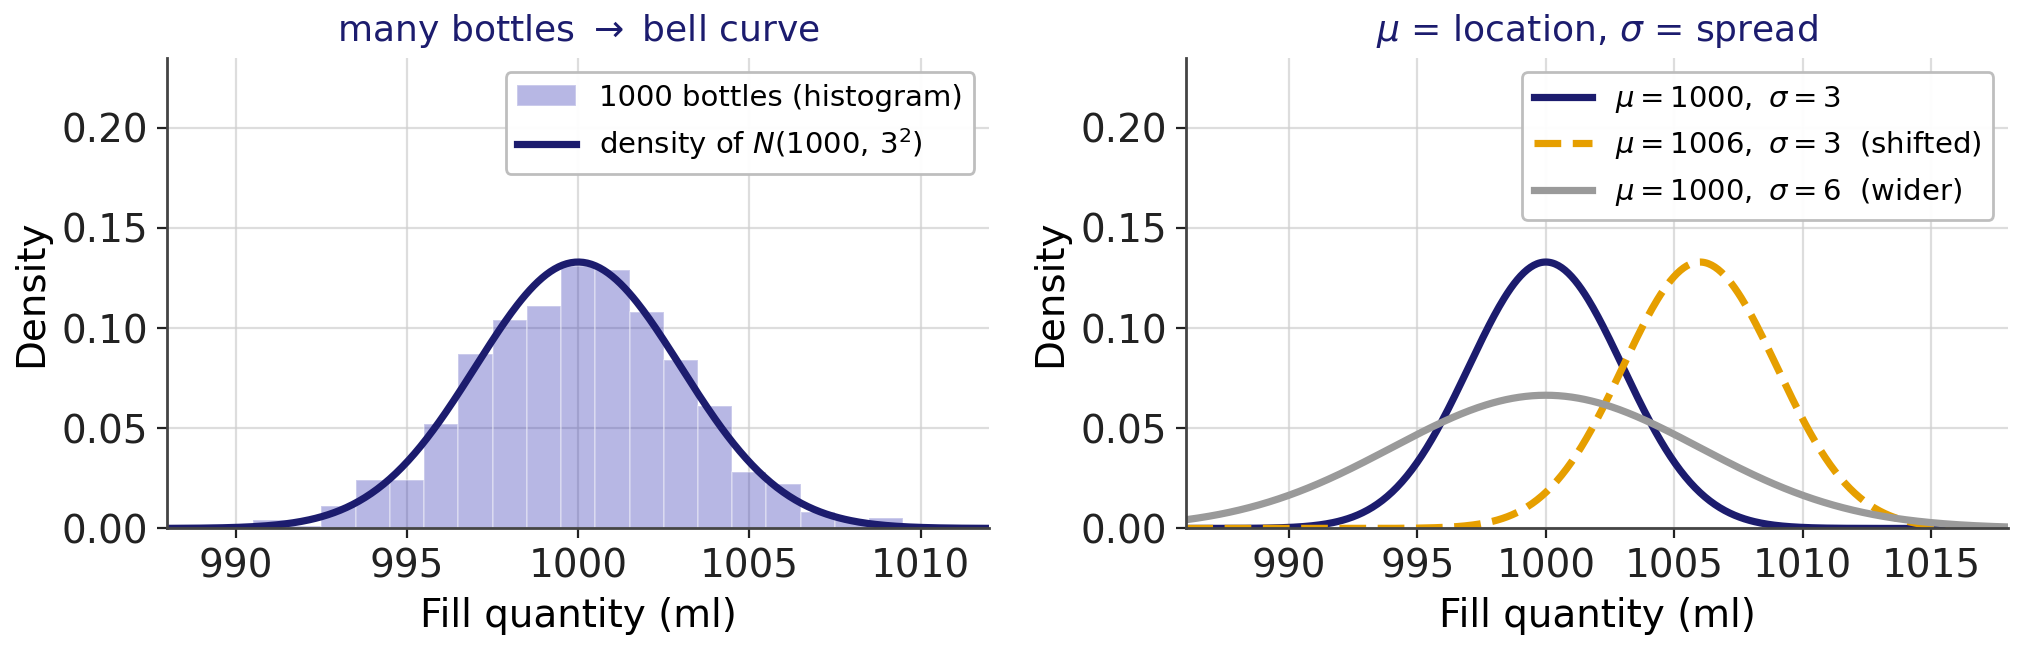
\includegraphics[width=\textwidth,height=0.50\textheight,keepaspectratio]{images/normal_bell.png}\par
  \raggedright
  \begin{columns}[T]
    \begin{column}{0.46\textwidth}
      \begin{block}{Density of $X\sim N(\mu,\sigma^2)$}
        \vspace{-2pt}
        \[ f(x)=\frac{1}{\sqrt{2\pi}\,\sigma}\;e^{-\frac{(x-\mu)^2}{2\sigma^2}},
           \quad x\in\mathbb{R} \]
        \vspace{-12pt}
      \end{block}
    \end{column}
    \begin{column}{0.50\textwidth}
      \footnotesize
      \begin{itemize}\setlength{\itemsep}{1pt}
        \item $E(X)=\mu$ (location), $\mathrm{Var}(X)=\sigma^2$ (spread);
              symmetric bell around $\mu$.
        \item Probabilities are \textbf{areas} under $f$.
        \item Careful: \texttt{scipy} wants the \emph{standard deviation},
              \texttt{stats.norm(loc=$\mu$, scale=$\sigma$)}.
      \end{itemize}
    \end{column}
  \end{columns}
\end{frame}
\note{Talk track: start with the left panel -- measure many bottles, the
histogram looks like a bell. The normal distribution is the idealised model
of such data. Right panel: $\mu$ moves the bell, $\sigma$ widens it (and
lowers it, because the area stays $1$). Repeat the convention: in this course
the second argument is the variance; scipy's \texttt{scale} is $\sigma$.}

% ---- Standardisation --------------------------------------------------------
\begin{frame}{Standardisation: one table for all normal distributions}
  \begin{block}{Standard normal distribution}
    $Z\sim N(0,1)$ has density $\varphi(z)$ and CDF $\Phi(z)=P(Z\le z)$.
    Normal areas have no closed formula, but every normal variable can be
    \textbf{standardised}:
    \[
      X\sim N(\mu,\sigma^2)\quad\Longrightarrow\quad
      Z=\frac{X-\mu}{\sigma}\sim N(0,1),\qquad\text{conversely } X=\mu+\sigma Z .
    \]
  \end{block}
  \begin{exampleblock}{Milk: a single bottle, $X\sim N(1000,\,3^2)$}
    \vspace{-6pt}
    \[
      P(X\le 997)=P\Bigl(Z\le\tfrac{997-1000}{3}\Bigr)=\Phi(-1)
      =1-\Phi(1)=1-0.8413=\mathbf{0.1587}
    \]
    \vspace{-12pt}\par
    $997$\,ml lies one standard deviation below $\mu$: about $16\,\%$ of the
    bottles hold at most $997$\,ml.
  \end{exampleblock}
  \kernaussage{Standardising reduces every normal probability to \emph{one}
  table -- that of $\Phi$.}
\end{frame}
\note{Talk track: ``$z$ = distance from the mean in standard deviations''
-- say it until it sticks. Work the milk example on the board: subtract
$\mu$, divide by $\sigma$, look up $\Phi(1)$, use symmetry. Point ahead: the
standardised mean (and later the test statistic) is exactly this move applied
to $\bar X$, with the standard error instead of $\sigma$.}

% ---- Four basic cases ---------------------------------------------------------
\begin{frame}{Probabilities as areas -- the four basic cases}
  \centering
  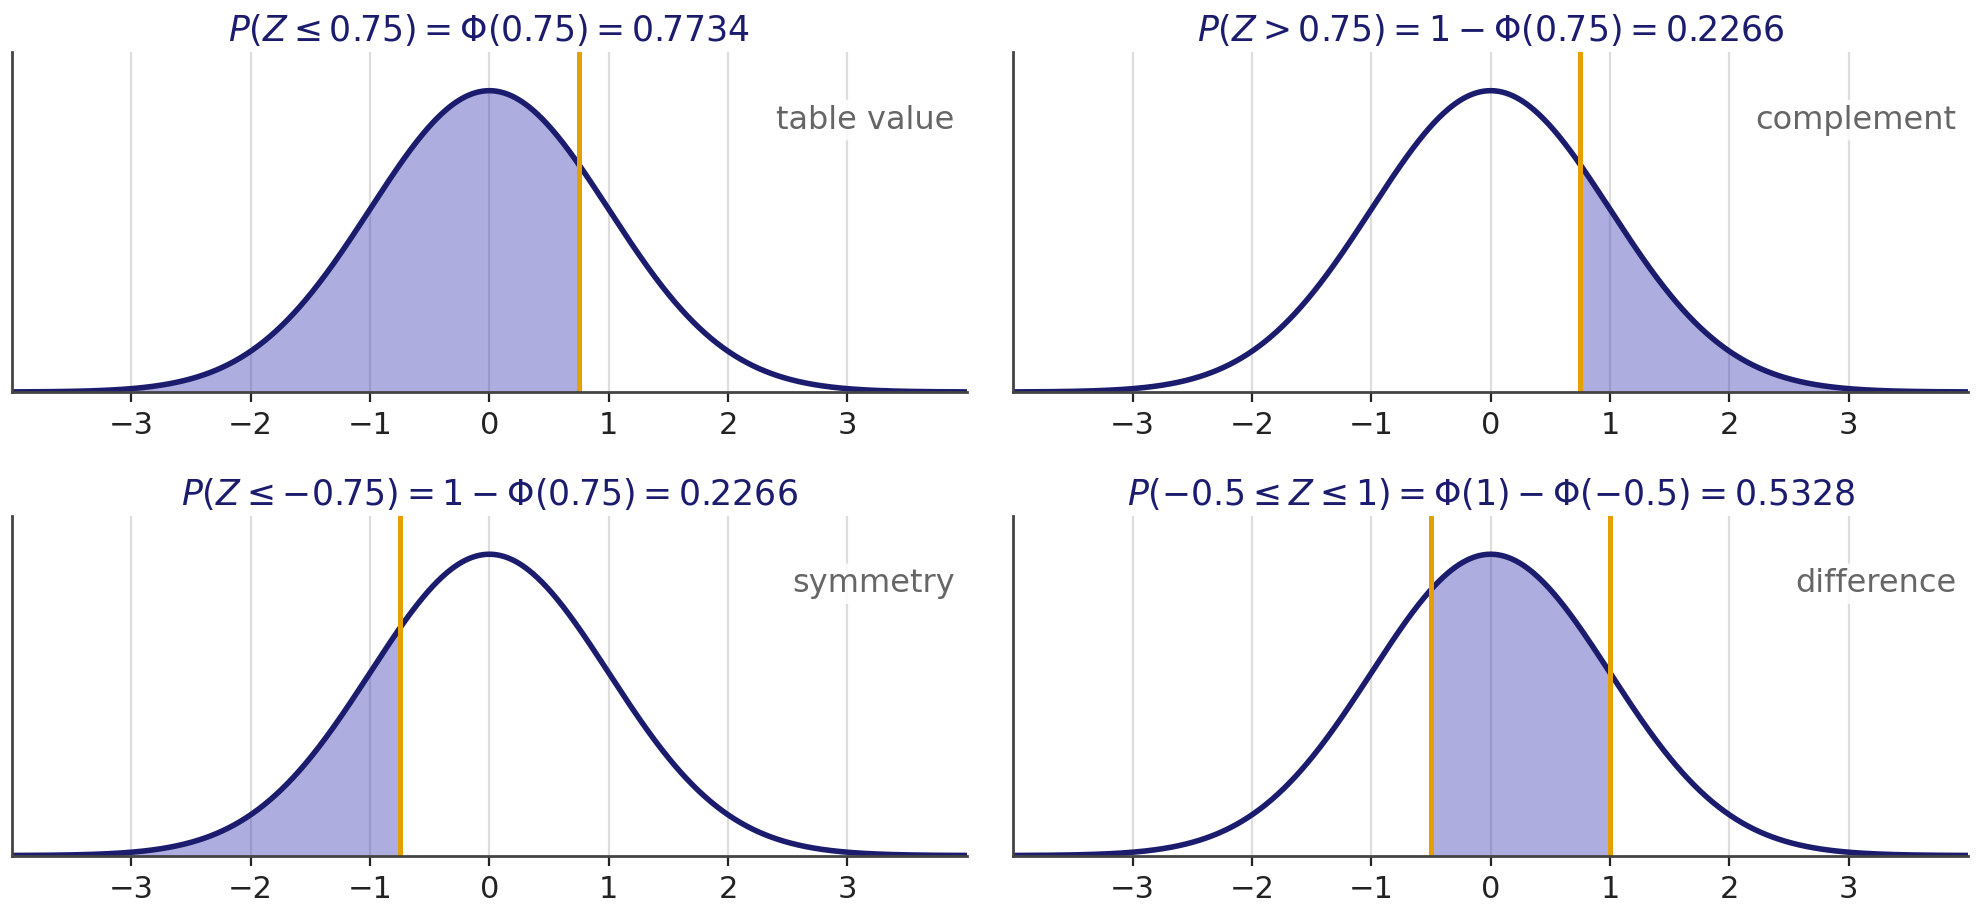
\includegraphics[width=0.92\textwidth,height=0.63\textheight,keepaspectratio]{images/normal_areas.png}\par
  \raggedright\footnotesize
  The table gives only $\Phi(z)=P(Z\le z)$. Everything else follows from
  \textbf{total area $=1$} and \textbf{symmetry}: \ $P(Z>z)=1-\Phi(z)$, \
  $\Phi(-z)=1-\Phi(z)$, \ $P(a\le Z\le b)=\Phi(b)-\Phi(a)$.
\end{frame}
\note{Talk track: ``draw before you calculate'' -- sketch the bell, shade
the area, then decide which rule applies. Ask: why is $P(Z>0.75)$ equal to
$P(Z\le-0.75)$? (symmetry). For continuous variables $P(Z=z)=0$, so $<$ and
$\le$ give the same probability.}

% ---- Phi table ----------------------------------------------------------------
\begin{frame}{Standard normal table $\Phi(z)=P(Z\le z)$ (1/2)}
  \begin{center}
    \scriptsize\setlength{\tabcolsep}{3.2pt}\renewcommand{\arraystretch}{0.96}
    \begin{tabular}{c|cccccccccc}
      \toprule
      $z$ & $.00$ & $.01$ & $.02$ & $.03$ & $.04$ & $.05$ & $.06$ & $.07$ & $.08$ & $.09$\\
      \midrule
      $0.0$ & 0.5000 & 0.5040 & 0.5080 & 0.5120 & 0.5160 & 0.5199 & 0.5239 & 0.5279 & 0.5319 & 0.5359 \\
      $0.1$ & 0.5398 & 0.5438 & 0.5478 & 0.5517 & 0.5557 & 0.5596 & 0.5636 & 0.5675 & 0.5714 & 0.5753 \\
      $0.2$ & 0.5793 & 0.5832 & 0.5871 & 0.5910 & 0.5948 & 0.5987 & 0.6026 & 0.6064 & 0.6103 & 0.6141 \\
      $0.3$ & 0.6179 & 0.6217 & 0.6255 & 0.6293 & 0.6331 & 0.6368 & 0.6406 & 0.6443 & 0.6480 & 0.6517 \\
      $0.4$ & 0.6554 & 0.6591 & 0.6628 & 0.6664 & 0.6700 & 0.6736 & 0.6772 & 0.6808 & 0.6844 & 0.6879 \\
      $0.5$ & 0.6915 & 0.6950 & 0.6985 & 0.7019 & 0.7054 & 0.7088 & 0.7123 & 0.7157 & 0.7190 & 0.7224 \\
      $0.6$ & 0.7257 & 0.7291 & 0.7324 & 0.7357 & 0.7389 & 0.7422 & 0.7454 & 0.7486 & 0.7517 & 0.7549 \\
      $0.7$ & 0.7580 & 0.7611 & 0.7642 & 0.7673 & 0.7704 & \cellcolor{hsbiorange!35}0.7734 & 0.7764 & 0.7794 & 0.7823 & 0.7852 \\
      $0.8$ & 0.7881 & 0.7910 & 0.7939 & 0.7967 & 0.7995 & 0.8023 & 0.8051 & 0.8078 & 0.8106 & 0.8133 \\
      $0.9$ & 0.8159 & 0.8186 & 0.8212 & 0.8238 & 0.8264 & 0.8289 & 0.8315 & 0.8340 & 0.8365 & 0.8389 \\
      $1.0$ & 0.8413 & 0.8438 & 0.8461 & 0.8485 & 0.8508 & 0.8531 & 0.8554 & 0.8577 & 0.8599 & 0.8621 \\
      $1.1$ & 0.8643 & 0.8665 & 0.8686 & 0.8708 & 0.8729 & 0.8749 & 0.8770 & 0.8790 & 0.8810 & 0.8830 \\
      $1.2$ & 0.8849 & 0.8869 & 0.8888 & 0.8907 & 0.8925 & 0.8944 & 0.8962 & 0.8980 & 0.8997 & 0.9015 \\
      $1.3$ & 0.9032 & 0.9049 & 0.9066 & 0.9082 & 0.9099 & 0.9115 & 0.9131 & 0.9147 & 0.9162 & 0.9177 \\
      $1.4$ & 0.9192 & 0.9207 & 0.9222 & 0.9236 & 0.9251 & 0.9265 & 0.9279 & 0.9292 & 0.9306 & 0.9319 \\
      \bottomrule
    \end{tabular}
  \end{center}
  {\footnotesize \textbf{Reading:} row $=$ $z$ to one decimal, column $=$
  second decimal. Highlighted: $z=0.75$ $\to$ row $0.7$, column $.05$ $\to$
  $\Phi(0.75)=0.7734$.}
\end{frame}

\begin{frame}{Standard normal table $\Phi(z)=P(Z\le z)$ (2/2)}
  \begin{center}
    \scriptsize\setlength{\tabcolsep}{3.2pt}\renewcommand{\arraystretch}{0.96}
    \begin{tabular}{c|cccccccccc}
      \toprule
      $z$ & $.00$ & $.01$ & $.02$ & $.03$ & $.04$ & $.05$ & $.06$ & $.07$ & $.08$ & $.09$\\
      \midrule
      $1.5$ & 0.9332 & 0.9345 & 0.9357 & 0.9370 & 0.9382 & 0.9394 & 0.9406 & 0.9418 & 0.9429 & 0.9441 \\
      $1.6$ & 0.9452 & 0.9463 & 0.9474 & 0.9484 & \cellcolor{hsbiorange!35}0.9495 & \cellcolor{hsbiorange!35}0.9505 & 0.9515 & 0.9525 & 0.9535 & 0.9545 \\
      $1.7$ & 0.9554 & 0.9564 & 0.9573 & 0.9582 & 0.9591 & 0.9599 & 0.9608 & 0.9616 & 0.9625 & 0.9633 \\
      $1.8$ & 0.9641 & 0.9649 & 0.9656 & 0.9664 & 0.9671 & 0.9678 & 0.9686 & 0.9693 & 0.9699 & 0.9706 \\
      $1.9$ & 0.9713 & 0.9719 & 0.9726 & 0.9732 & 0.9738 & 0.9744 & \cellcolor{hsbiorange!35}0.9750 & 0.9756 & 0.9761 & 0.9767 \\
      $2.0$ & 0.9772 & 0.9778 & 0.9783 & 0.9788 & 0.9793 & 0.9798 & 0.9803 & 0.9808 & 0.9812 & 0.9817 \\
      $2.1$ & 0.9821 & 0.9826 & 0.9830 & 0.9834 & 0.9838 & 0.9842 & 0.9846 & 0.9850 & 0.9854 & 0.9857 \\
      $2.2$ & 0.9861 & 0.9864 & 0.9868 & 0.9871 & 0.9875 & 0.9878 & 0.9881 & 0.9884 & 0.9887 & 0.9890 \\
      $2.3$ & 0.9893 & 0.9896 & 0.9898 & 0.9901 & 0.9904 & 0.9906 & 0.9909 & 0.9911 & 0.9913 & 0.9916 \\
      $2.4$ & 0.9918 & 0.9920 & 0.9922 & 0.9925 & 0.9927 & 0.9929 & 0.9931 & 0.9932 & 0.9934 & 0.9936 \\
      $2.5$ & 0.9938 & 0.9940 & 0.9941 & 0.9943 & 0.9945 & 0.9946 & 0.9948 & 0.9949 & 0.9951 & 0.9952 \\
      $2.6$ & 0.9953 & 0.9955 & 0.9956 & 0.9957 & 0.9959 & 0.9960 & 0.9961 & 0.9962 & 0.9963 & 0.9964 \\
      $2.7$ & 0.9965 & 0.9966 & 0.9967 & 0.9968 & 0.9969 & 0.9970 & 0.9971 & 0.9972 & 0.9973 & 0.9974 \\
      $2.8$ & 0.9974 & 0.9975 & 0.9976 & 0.9977 & 0.9977 & 0.9978 & 0.9979 & 0.9979 & 0.9980 & 0.9981 \\
      $2.9$ & 0.9981 & 0.9982 & 0.9982 & 0.9983 & 0.9984 & 0.9984 & 0.9985 & 0.9985 & 0.9986 & 0.9986 \\
      \bottomrule
    \end{tabular}
  \end{center}
  {\footnotesize Negative $z$ via symmetry: $\Phi(-z)=1-\Phi(z)$. For
  $z\ge 3$: $\Phi(z)\approx 1$. Highlighted: the quantiles $1.645$ and $1.96$
  (next slide).}
\end{frame}

% ---- Reading forwards / backwards ---------------------------------------------
\begin{frame}[fragile]{Reading the table -- forwards and backwards}
  \begin{columns}[T]
    \begin{column}{0.48\textwidth}
      \begin{block}{Forwards: probability wanted}
        \small
        $z=0.75$: row $0.7$, column $.05$ $\Rightarrow$
        $\Phi(0.75)=\mathbf{0.7734}$.\\[2pt]
        Negative $z$: $\Phi(-0.75)=1-0.7734=0.2266$.
      \end{block}
    \end{column}
    \begin{column}{0.48\textwidth}
      \begin{block}{Backwards: quantile wanted}
        \small
        Search $0.95$ \emph{inside} the table: $\Phi(1.64)=0.9495$,
        $\Phi(1.65)=0.9505$ $\Rightarrow$ $z_{0.95}\approx\mathbf{1.645}$.\\[2pt]
        $\Phi(1.96)=0.9750$ $\Rightarrow$ $z_{0.975}=\mathbf{1.96}$.
      \end{block}
    \end{column}
  \end{columns}
  {\small The \textbf{$p$-quantile} $z_p$ is defined by $\Phi(z_p)=p$; by
  symmetry $z_{1-p}=-z_p$ (e.g.\ $z_{0.05}=-1.645$).}
\begin{lstlisting}
from scipy import stats
stats.norm.cdf(0.75)                     # Phi(0.75)              -> 0.7734
stats.norm.ppf(0.95)                     # quantile z_0.95        -> 1.6449
stats.norm.cdf(997, loc=1000, scale=3)   # P(X <= 997), N(1000,9) -> 0.1587
\end{lstlisting}
  \kernaussage{The famous $1.96$ is the $0.975$-quantile of $N(0,1)$: the
  central $95\,\%$ of the area lies between $\pm1.96$.}
  \trynotebook{section 1.2 ``Normal distribution''}
\end{frame}
\note{Talk track: forwards = look up the margin, read inside; backwards =
look up inside, read the margin. Let students find $1.96$ themselves in the
(2/2) table -- the ``magic number'' of the next section loses its mystery.
\texttt{cdf} goes forwards, \texttt{ppf} (percent point function) goes
backwards.}

% ---- Exercise: fill volume --------------------------------------------------------
\begin{frame}{Exercise -- normal distribution: fill volume}
  \begin{block}{Problem statement}
    A bottling plant fills orange juice into 1-litre bottles. The fill volume
    $X$ (in ml) is normally distributed with $\mu=1000$ and $\sigma=10$, i.e.\
    $X\sim N(1000,\,10^2)$. The legal minimum content is $985$\,ml.
  \end{block}
  \begin{enumerate}\setlength{\itemsep}{3pt}
    \item[a)] What share of the bottles is underfilled, $P(X<985)$?
    \item[b)] With what probability does a bottle contain between $990$ and
              $1015$\,ml?
    \item[c)] Which fill volume $x_{0.95}$ is exceeded by only $5\,\%$ of the
              bottles?
    \item[d)] The share of underfilled bottles is to be cut to at most
              $1\,\%$. To which setpoint $\mu$ must the plant be adjusted if
              $\sigma=10$ stays the same?
  \end{enumerate}
  \textbf{Hint:} standardise, $z=(x-\mu)/\sigma$, and use the $\Phi$ table.
\end{frame}
\note{Talk track: give 5--7 minutes. Insist on a sketch of the bell curve
for every part -- a) and b) are areas (forwards), c) and d) are quantiles
(backwards). Part d) is the business punchline: the safety margin costs juice
in every single bottle.}

\begin{frame}{Solution (1/3) -- fill volume: probabilities}
  \textbf{Rules:} $P(X\le x)=\Phi\bigl(\tfrac{x-\mu}{\sigma}\bigr)$; \
  $\Phi(-z)=1-\Phi(z)$; \ $P(a\le X\le b)=\Phi(z_b)-\Phi(z_a)$.
  \begin{align*}
    \text{a)}\quad P(X<985) &= \Phi\Bigl(\tfrac{985-1000}{10}\Bigr)=\Phi(-1.5)
      =1-\Phi(1.5)=1-0.9332=\mathbf{0.0668}\\[4pt]
    \text{b)}\quad P(990\le X\le 1015)
      &=\Phi\Bigl(\tfrac{1015-1000}{10}\Bigr)-\Phi\Bigl(\tfrac{990-1000}{10}\Bigr)
       =\Phi(1.5)-\Phi(-1)\\
      &=0.9332-(1-0.8413)=0.9332-0.1587=\mathbf{0.7745}
  \end{align*}
  \begin{exampleblock}{Interpretation}
    About $6.7\,\%$ of the bottles are underfilled; about $77.5\,\%$ contain
    between $990$ and $1015$\,ml.
  \end{exampleblock}
\end{frame}

\begin{frame}{Solution (2/3) -- fill volume: quantile and setpoint}
  \textbf{Rules:} quantile $x_p=\mu+\sigma z_p$ (search $p$ \emph{inside} the
  table); \ $z_{1-p}=-z_p$.
  \begin{align*}
    \text{c)}\quad &\Phi(z)=0.95\ \Rightarrow\ z_{0.95}=1.645
       \ \Rightarrow\ x_{0.95}=1000+1.645\cdot10=\mathbf{1016.45\ ml}\\[4pt]
    \text{d)}\quad &P(X<985)=0.01\ \Rightarrow\
       \tfrac{985-\mu}{10}=z_{0.01}=-z_{0.99}\approx-2.33
       \quad(\text{table: }\Phi(2.33)=0.9901)\\
     &\Rightarrow\ \mu=985+2.33\cdot10=\mathbf{1008.3\ ml}
       \quad(\text{exact } z_{0.99}=2.3263:\ 1008.26\text{ ml})
  \end{align*}
  \begin{exampleblock}{Interpretation}
    Only $5\,\%$ of the bottles contain more than $1016.45$\,ml. To cut
    underfilling from $6.7\,\%$ to $1\,\%$, the setpoint must rise by about
    $8$\,ml -- every bottle gets more juice: the price of safety.
  \end{exampleblock}
\end{frame}

\begin{frame}[fragile]{Solution (3/3) -- fill volume: with Python}
  \textbf{Rule:} \texttt{cdf} gives $P(X\le x)$, \texttt{ppf} the quantile;
  \texttt{scale} $=\sigma$ is the \emph{standard deviation}.
\begin{lstlisting}
from scipy import stats

X = stats.norm(loc=1000, scale=10)          # X ~ N(1000, 10^2)
print(f"a) {X.cdf(985):.4f}")
print(f"b) {X.cdf(1015) - X.cdf(990):.4f}")
print(f"c) {X.ppf(0.95):.2f}")
print(f"d) {985 - stats.norm.ppf(0.01) * 10:.2f}")   # mu = 985 - z_0.01 * sigma
\end{lstlisting}
  \begin{columns}[T]
    \begin{column}{0.36\textwidth}
      \begin{block}{Output}
\begin{lstlisting}[style=Pyout]
a) 0.0668
b) 0.7745
c) 1016.45
d) 1008.26
\end{lstlisting}
      \end{block}
    \end{column}
    \begin{column}{0.60\textwidth}
      \footnotesize The table answers differ only by rounding
      ($z_{0.99}=2.33$ instead of $2.3263$ in d).
    \end{column}
  \end{columns}
  \trynotebook{section 1.2 ``Normal distribution''}
\end{frame}

\subsection{Sampling distribution and CLT}

% ---- Sampling distribution: estimators are random variables ----------------
\begin{frame}{Estimators are random variables}
  \small The sample $X_1,\dots,X_n$ is \textbf{random}, so \emph{anything}
  computed from it -- $\bar X$, $s$, and later the test statistics -- is itself
  a \textbf{random variable}.
  \begin{itemize}\small\setlength{\itemsep}{2pt}
    \item New sample $\Rightarrow$ a new $\bar x$ \emph{and} a new $s$.
    \item Its distribution over \emph{all possible samples} is the
          \textbf{sampling distribution} -- so $\bar X$ and $s$ each have
          their own.
  \end{itemize}
  \begin{center}
  \begin{tikzpicture}
    \node[flowboxo, text width=2.6cm] (s) {\footnotesize random sample\\ $X_1,\dots,X_n$};
    \node[flowbox, text width=2.4cm, right=16mm of s] (st) {\footnotesize statistic\\ $\bar X$ \ or\ $s$};
    \node[flowboxg, text width=2.8cm, right=16mm of st] (d) {\footnotesize \textbf{sampling}\\ \textbf{distribution}};
    \draw[flowarr] (s) -- (st)
      node[midway,above=1pt,font=\scriptsize,fill=white,inner sep=1.5pt]{compute};
    \draw[flowarr] (st) -- (d)
      node[midway,above=1pt,font=\scriptsize,fill=white,inner sep=1.5pt]{repeat};
  \end{tikzpicture}
  \end{center}
  \kernaussage{A confidence interval or test is built on the \emph{sampling
  distribution} of an estimator -- never on a single number alone.}
\end{frame}

% ---- Standard error -------------------------------------------------------
\begin{frame}{The standard error: how much $\bar X$ wobbles}
  \begin{block}{Definition}
    The \textbf{standard error} (SE) is the \emph{standard deviation of the
    sampling distribution} of an estimator -- the spread of $\bar X$ from
    sample to sample, \emph{not} the spread of the raw data.
    \[
      \mathrm{SE}(\bar X)=\sqrt{\mathrm{Var}(\bar X)}=\frac{\sigma}{\sqrt n}\quad
      \Bigl(\text{or }\tfrac{s}{\sqrt n}\text{ when }\sigma\text{ is estimated}\Bigr).
    \]
  \end{block}
  \begin{itemize}\setlength{\itemsep}{2pt}
    \item It is the natural \textbf{ruler} for inference: we will measure
          \emph{how many standard errors} $\bar x$ lies away from a reference
          value -- this standardised quantity reappears as the test statistic
          in Section~3.
    \item Larger $n$ $\Rightarrow$ smaller SE $\Rightarrow$ narrower CI and
          sharper test.
  \end{itemize}
  \kernaussage{Standard \emph{deviation} = spread of the data; \quad standard
  \emph{error} = spread of the estimate.}
\end{frame}

% ---- CLT: intuition -------------------------------------------------------------
\begin{frame}{The central limit theorem -- intuition}
  \guidingquestion{Our inference rests on $\bar X\sim N(\mu,\sigma^2/n)$. But
  real data -- waiting times, incomes, processing times -- are often
  \emph{skewed}. Does the recipe still work?}
  \begin{itemize}\setlength{\itemsep}{2pt}
    \item Draw $n$ independent values from \emph{any} distribution (skewed,
          flat, bimodal) with mean $\mu$ and standard deviation $\sigma$.
    \item Their \textbf{mean} $\bar X$ is approximately \textbf{normal} once
          $n$ is large enough -- the shape of the original distribution washes
          out.
    \item Why? In an average, unusually high and unusually low values partly
          cancel out; what remains is a symmetric bell around $\mu$.
  \end{itemize}
  \kernaussage{Whatever the shape of the data: for large $n$ the
  \textbf{sample mean} is approximately normal, with centre $\mu$ and
  standard error $\sigma/\sqrt n$.}
\end{frame}
\note{Talk track: ask first -- ``waiting times at a checkout are skewed;
is the AVERAGE waiting time of 50 customers skewed too?'' Let them guess, then
show the simulation on the next slide. Keep the distinction sharp: the CLT is
about averages (and sums), never about single observations.}

% ---- CLT: simulation ------------------------------------------------------------
\begin{frame}{The central limit theorem -- a simulation}
  \centering
  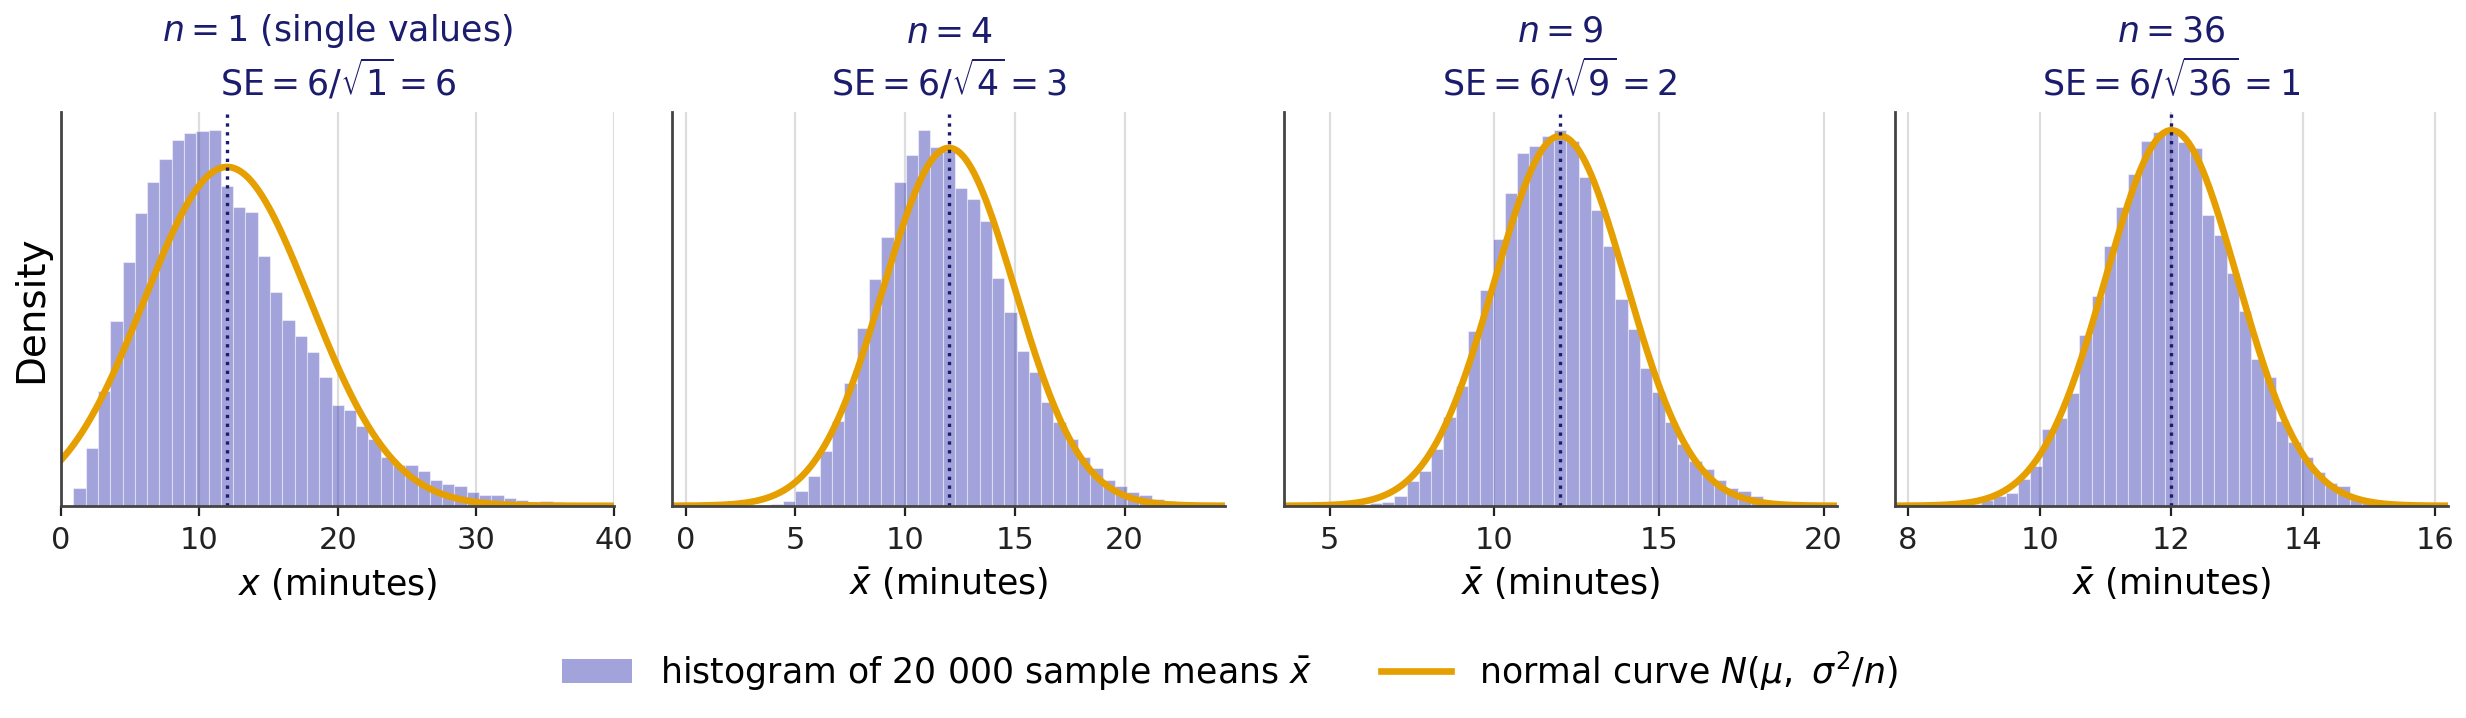
\includegraphics[width=\textwidth,height=0.56\textheight,keepaspectratio]{images/clt_simulation.png}\par
  \raggedright\footnotesize
  Processing times of customer orders are right-skewed (here: gamma
  distribution with $\mu=12$, $\sigma=6$ minutes). For each $n$, $20\,000$
  samples were drawn and their means $\bar x$ plotted. For $n=1$ the normal
  curve fits badly; at $n=36$ the histogram of $\bar x$ is practically normal
  -- and it narrows like $6/\sqrt n$.
\end{frame}
\note{Talk track: read the panels from left to right. Left: single values,
clearly skewed -- the orange normal curve is wrong. Each step to the right:
the histogram becomes more symmetric AND narrower. Two messages in one
picture: the shape becomes normal (CLT) and the spread shrinks like
$1/\sqrt n$ (standard error). Seed and code are in \texttt{make\_figures.py}.}

% ---- CLT: formal ----------------------------------------------------------------
\begin{frame}{The central limit theorem -- formal statement}
  \begin{block}{Central limit theorem (Lindeberg--L\'evy)}
    Let $X_1,\dots,X_n$ be i.i.d.\ with $E(X_i)=\mu$ and
    $0<\mathrm{Var}(X_i)=\sigma^2<\infty$. Then
    \[
      Z_n=\frac{\bar X-\mu}{\sigma/\sqrt n}\ \xrightarrow{\;d\;}\ N(0,1)
      \quad (n\to\infty),
      \qquad\text{i.e.}\qquad
      \bar X\ \overset{\text{approx.}}{\sim}\ N\Bigl(\mu,\frac{\sigma^2}{n}\Bigr).
    \]
  \end{block}
  \inworten{For large $n$ the standardised mean behaves like a standard
  normal variable -- whatever the distribution of the single values.}
  \begin{itemize}\small\setlength{\itemsep}{1pt}
    \item $\xrightarrow{d}$ = convergence \emph{in distribution}: the CDF of
          $Z_n$ approaches $\Phi$.
    \item Rule of thumb: $n\gtrsim 30$ is usually enough; strongly skewed data
          need more.
    \item For \emph{normal} data, $\bar X\sim N(\mu,\sigma^2/n)$ holds
          \emph{exactly}, for every $n$.
    \item The CLT is about $\bar X$ -- it does \emph{not} make the single
          values normal.
  \end{itemize}
\end{frame}
\note{Talk track: connect to what follows -- every CI and test in this part
standardises $\bar X$ like $Z_n$; the CLT is the licence to do so for non-normal data with
$n\gtrsim30$ (assumptions checklist later). Typical exam trap: ``by the CLT
the data are normal'' -- no, only the mean is.}

% ---- CLT with Python (simulation) ---------------------------------------------
\begin{frame}[fragile]{The central limit theorem with Python}
  \textbf{Simulation:} $20\,000$ shifts with $n=36$ right-skewed processing
  times each (gamma distribution with $\mu=12$, $\sigma=6$ minutes, as on the
  simulation slide).
\begin{lstlisting}
import numpy as np
from scipy import stats
rng = np.random.default_rng(42)                          # fixed seed
times = rng.gamma(shape=4, scale=3, size=(20_000, 36))   # 20 000 shifts x 36 orders
means = times.mean(axis=1)                               # one mean per shift
times.mean(), times.std()                     # single values:  12.0, 6.0
means.mean(), means.std()                     # shift means:    12.003, 0.99
stats.skew(times.ravel()), stats.skew(means)  # skewness:       1.0, 0.15
np.mean(means > 13.5)                         # share of shifts above 13.5 min: 0.0698
stats.norm.sf(13.5, loc=12, scale=6 / np.sqrt(36))      # CLT approximation:  0.0668
\end{lstlisting}
  \inworten{The shift means are centred at $\mu=12$, spread with
  $\sigma/\sqrt n=1$ and are almost symmetric (skewness $1.0\to0.15$),
  although every single time is right-skewed. The simulated share above
  $13.5$ minutes is close to the CLT value.}
  \trynotebook{section 1.3 ``Sampling distribution and CLT''}
\end{frame}
\note{Talk track: the simulation slide in code. Point at the three pairs of
numbers -- centre stays, spread shrinks by $\sqrt{36}=6$, skewness almost
vanishes. Students can change $n$ in the notebook (e.g.\ $n=4$) and watch the
skewness come back.}

% ---- Exercise: CLT --------------------------------------------------------------
\begin{frame}{Exercise -- central limit theorem: processing times}
  \begin{block}{Problem statement}
    The processing time $X$ of a customer order in a service centre (in
    minutes) is \textbf{right-skewed}; its exact distribution is unknown.
    Known are only $\mu=12$ and $\sigma=6$. In one shift, $n=36$ orders are
    processed independently of each other.
  \end{block}
  \begin{enumerate}\setlength{\itemsep}{3pt}
    \item[a)] How is the mean processing time $\bar X$ of a shift
              (approximately) distributed? Why?
    \item[b)] With what probability is the mean processing time of a shift
              above $13.5$ minutes?
    \item[c)] What would $P(X>13.5)$ be for a \emph{single} order if $X$ were
              normal? Why can this not be computed without that assumption --
              whereas b) can?
    \item[d)] How many orders per shift would be needed for a standard error of
              the mean of at most $0.5$ minutes?
  \end{enumerate}
\end{frame}

\begin{frame}{Solution (1/3) -- processing times: distribution of the mean}
  \textbf{Rule (CLT):} for i.i.d.\ $X_i$ and large $n$,
  $\bar X\overset{\text{approx.}}{\sim}N(\mu,\sigma^2/n)$ -- whatever the
  shape of the distribution of $X$.
  \begin{align*}
    \text{a)}\quad & E(\bar X)=12,\qquad
      \mathrm{SE}=\frac{\sigma}{\sqrt n}=\frac{6}{\sqrt{36}}=1
      \quad\Rightarrow\quad \bar X\overset{\text{approx.}}{\sim}\mathbf{N(12,\,1^2)}\\[4pt]
    \text{b)}\quad & P(\bar X>13.5)=P\Bigl(Z>\tfrac{13.5-12}{1}\Bigr)
      =1-\Phi(1.5)=1-0.9332=\mathbf{0.0668}
  \end{align*}
  \begin{exampleblock}{Interpretation}
    Although single processing times are skewed, the mean of $36$ orders is
    approximately normal ($n=36\ge30$). Only in about $6.7\,\%$ of the shifts
    does the mean processing time exceed $13.5$ minutes.
  \end{exampleblock}
\end{frame}

\begin{frame}{Solution (2/3) -- processing times: single value vs.\ mean}
  \textbf{Rule:} $P(X>x)=1-\Phi\bigl(\tfrac{x-\mu}{\sigma}\bigr)$ for a
  \emph{single} value holds \textbf{only} if $X$ itself is normal -- the CLT
  says nothing about $X$, only about $\bar X$.
  \[
    \text{c)}\quad P(X>13.5)=1-\Phi\Bigl(\tfrac{13.5-12}{6}\Bigr)
      =1-\Phi(0.25)=1-0.5987=\mathbf{0.4013}
  \]
  \vspace{-6pt}
  \centerline{\small (valid \emph{only} if $X$ itself is normal)}
  \begin{itemize}\small\setlength{\itemsep}{2pt}
    \item For a skewed $X$ with the same $\mu$ and $\sigma$ the true value can
          differ markedly. Example: under the gamma model of the simulation
          slide, $P(X>13.5)=0.342$ -- not $0.401$.
    \item $P(\bar X>13.5)=0.0668$ is reliable: the CLT delivers the normal
          shape of the mean \emph{without} knowing the shape of $X$ (gamma
          model, exact: $0.071$).
  \end{itemize}
  \kernaussage{A single order exceeds $13.5$ minutes often (roughly $35$--$40\,\%$),
  the shift mean rarely ($\approx7\,\%$): averaging shrinks the spread by the
  factor $\sqrt{36}=6$.}
\end{frame}

\begin{frame}[fragile]{Solution (3/3) -- processing times: sample size and Python}
  \textbf{Rule:} $\mathrm{SE}=\sigma/\sqrt n$ -- the standard error falls with
  $\sqrt n$, not with $n$.
  \begin{columns}[T]
    \begin{column}{0.58\textwidth}
      \[
        \text{d)}\quad \frac{6}{\sqrt n}\le 0.5
        \;\Leftrightarrow\; \sqrt n\ge\frac{6}{0.5}=12
        \;\Leftrightarrow\; n\ge \mathbf{144}
      \]
      \inworten{Halving the standard error (from $1$ to $0.5$ minutes)
      requires four times as many orders ($36\to144$).}
    \end{column}
    \begin{column}{0.38\textwidth}
      \begin{block}{Output (code below)}
\begin{lstlisting}[style=Pyout]
b) 0.0668
c) 0.4013
d) 144
\end{lstlisting}
      \end{block}
    \end{column}
  \end{columns}
\begin{lstlisting}
import numpy as np
from scipy import stats

print(f"b) {stats.norm.sf(13.5, loc=12, scale=6 / np.sqrt(36)):.4f}")  # mean
print(f"c) {stats.norm.sf(13.5, loc=12, scale=6):.4f}")   # single value, IF normal
print(f"d) {(6 / 0.5) ** 2:.0f}")
\end{lstlisting}
  \trynotebook{section 1.3 ``Sampling distribution and CLT''}
\end{frame}

% ============================================================================
% SECTION 2: CONFIDENCE INTERVALS
% ============================================================================
\section[CIs]{Confidence Intervals}

\subsection{Motivation and intuition}


% ---- Intuition: a point estimate is not enough -----------------------------
\begin{frame}{A single estimate is not enough}
  \begin{block}{Intuition}
    From the sample we compute the mean $\bar x$. But it almost \textbf{never}
    hits the true value $\mu$ exactly -- a second sample would give a
    different value.
  \end{block}
  \begin{itemize}
    \item Instead of a single point we report a \textbf{range} of values that
          are \emph{compatible with the data}.
    \item The more precise our estimate, the \emph{narrower} this range.
  \end{itemize}
  \kernaussage{A \textbf{confidence interval} reports the estimate
  \emph{together with its uncertainty} -- a range of plausible values for
  $\mu$. (It is \emph{not} a probability statement about where $\mu$ lies --
  see the interpretation slides.)}
\end{frame}

% ---- Estimation chain (TikZ) -----------------------------------------------
\begin{frame}{From the sample to the interval}
  \centering
  \resizebox{\textwidth}{!}{%
  \begin{tikzpicture}[node distance=22mm and 20mm]
    \node[flowboxo, text width=2.4cm] (st) {\footnotesize Sample\\ $x_1,\dots,x_n$};
    \node[flowbox, text width=2.5cm, right=of st] (ps)
      {\footnotesize \textbf{Point estimator}\\ $\bar x$};
    \node[flowbox, text width=3.2cm, right=of ps] (ki)
      {\footnotesize \textbf{Interval estimator}\\ $[\,\bar x - e,\ \bar x + e\,]$};
    \node[flowboxg, text width=2.2cm, right=of ki] (mu)
      {\footnotesize Parameter\\ $\mu$};
    \draw[flowarr] (st) -- (ps)
      node[midway,above,font=\scriptsize,fill=white,inner sep=2pt]{average};
    \draw[flowarr] (ps) -- (ki)
      node[midway,above,font=\scriptsize,align=center,fill=white,inner sep=2pt]{$+$ uncertainty};
    \draw[flowarr, draw=hsbiorange!85!black] (ki) -- (mu)
      node[midway,above,font=\scriptsize,fill=white,inner sep=2pt]{covers};
  \end{tikzpicture}}
  \vspace{1.2em}
  \begin{itemize}
    \item The point estimator $\bar x$ is the \emph{best single estimate}.
    \item The \emph{margin of error} $e=z_{1-\alpha/2}\,\sigma/\sqrt n$ (half
          the interval's width) turns it into an interval -- built so that the
          \emph{procedure} covers the fixed true $\mu$ in $(1-\alpha)$ of
          samples.
  \end{itemize}
\end{frame}



% ---- Why standardise -------------------------------------------------------
\begin{frame}{Why divide by the standard error?}
  \begin{block}{The raw deviation is not enough}
    A sample mean $\bar x = 8$ lies $2$ units from a reference value
    $\mu_0=10$. Whether that gap is \emph{small or large} depends entirely on
    the standard error -- how much $\bar X$ wobbles.
  \end{block}
  \begin{center}
    \renewcommand{\arraystretch}{1.3}
    \begin{tabular}{lccc}
      \toprule
      Scenario & $\mathrm{SE}=\sigma/\sqrt n$ & $z=\dfrac{8-10}{\mathrm{SE}}$ & Reading\\
      \midrule
      large spread, small $n$ \ ($\sigma=6,\ n=9$)   & $2.0$ & $-1.0$ & ordinary\\
      small spread, large $n$ \ ($\sigma=4,\ n=100$) & $0.4$ & $-5.0$ & far out\\
      \bottomrule
    \end{tabular}
  \end{center}
  \kernaussage{Same raw deviation, opposite readings. Dividing by the SE turns
  it into a \emph{universal} ruler -- ``how many standard errors'' -- comparable
  across samples and units.}
\end{frame}
\note{Talk track: walk the table row by row -- same gap of $2$ units, but in
row 1 the mean typically wobbles by $2$ anyway (nothing special), while in
row 2 it wobbles by $0.4$, so a gap of $2$ is five wobbles away (very
unusual). This is THE reason every test statistic in this course has the same
shape: (estimate $-$ hypothesised) / SE.}

% ---- Quick exercise: standard error (SfOe Teil 6) --------------------------------
\begin{frame}{Exercise -- standard error: packing flour}
  \begin{block}{Problem statement}
    A mill packs flour into $500$\,g bags. The single bags scatter with a
    known standard deviation of $\sigma=8$\,g.
  \end{block}
  \begin{enumerate}\setlength{\itemsep}{4pt}
    \item[a)] What is the standard error of $\bar X$ for $n=16$ and for
              $n=64$ bags?
    \item[b)] A sample gives $\bar x=497$\,g. How many standard errors does
              $\bar x$ lie below the target $\mu_0=500$\,g -- for $n=16$ and
              for $n=64$? Which finding is conspicuous?
    \item[c)] How much do the \emph{single} bags scatter if $64$ instead of
              $16$ bags are drawn?
  \end{enumerate}
  \textbf{Hint:} the central $95\,\%$ of $N(0,1)$ lie between $\pm1.96$;
  $\Phi(1.50)=0.9332$.
\end{frame}
\note{Talk track: three minutes, numbers chosen for mental arithmetic. The
same $3$\,g shortfall is harmless at $n=16$ and alarming at $n=64$ -- exactly
the message of the previous slide. Part c) catches the classic confusion of
standard deviation and standard error.}

\begin{frame}{Solution -- standard error: packing flour}
  \textbf{Rule:} $\mathrm{SE}=\sigma/\sqrt n$; \ distance in standard errors:
  $z=(\bar x-\mu_0)/\mathrm{SE}$.
  \begin{center}
    \renewcommand{\arraystretch}{1.3}
    \begin{tabular}{lcc}
      \toprule
       & $n=16$ & $n=64$\\
      \midrule
      a) \ $\mathrm{SE}=\sigma/\sqrt n$
        & $8/\sqrt{16}=8/4=\mathbf{2\ g}$
        & $8/\sqrt{64}=8/8=\mathbf{1\ g}$\\
      b) \ $z=(497-500)/\mathrm{SE}$
        & $-3/2=\mathbf{-1.5}$
        & $-3/1=\mathbf{-3.0}$\\
      \phantom{b) \ }reading
        & $|z|<1.96$: ordinary fluctuation
        & \textcolor{hsbirot}{$|z|>1.96$: conspicuous}\\
      \bottomrule
    \end{tabular}
  \end{center}
  {\small For $n=16$, a deviation of at least $1.5$ standard errors occurs in
  $2\,(1-\Phi(1.50))=2\cdot0.0668=0.1336$, i.e.\ in about $13\,\%$ of all
  samples; $3$ standard errors lie beyond the central $95\,\%$.\par}
  \smallskip
  \textbf{c)} Unchanged, $\mathbf{\sigma=8\ g}$ -- a larger $n$ shrinks only
  the spread of the \emph{mean}, not that of the data.
  \kernaussage{Same $3$\,g shortfall, opposite verdicts: it is the distance
  in \textbf{standard errors} that counts.}
\end{frame}

% ---- Frequentist paradigm --------------------------------------------------
\begin{frame}{How we read probability: the frequentist view}
  \begin{columns}[T]
    \begin{column}{0.48\textwidth}
      \begin{block}{Fixed vs.\ random}
        \begin{itemize}\footnotesize\setlength{\itemsep}{2pt}
          \item Parameters $\mu,\sigma$ are \textbf{fixed} (unknown) constants
                -- not random.
          \item The data -- and all we build from them ($\bar X$, $s$, $Z_n$,
                the CI bounds, later the test results) -- are
                \textbf{random}.
        \end{itemize}
      \end{block}
    \end{column}
    \begin{column}{0.48\textwidth}
      \begin{block}{What ``probability'' means here}
        \footnotesize The long-run \emph{relative frequency} of an event over
        (hypothetically) very many repeated samples.
      \end{block}
    \end{column}
  \end{columns}
  \kernaussage{``$95\,\%$ confidence'' and ``$5\,\%$ significance'' describe
  the \textbf{procedure across repeated samples} -- not one particular interval
  and not one particular dataset.}
  \appendixnote{law of large numbers -- why relative frequencies settle down}
\end{frame}
\note{Talk track: this slide is the philosophical key to the whole part --
return to it whenever an interpretation question comes up. Anchor sentence:
``$\mu$ does not move; OUR numbers move from sample to sample.'' The casino
analogy works well: a casino cannot predict one evening, but it knows its
long-run win rate -- our procedures are calibrated the same way.}

\subsection{Known variance}

% ---- Milk example setup ----------------------------------------------------
\begin{frame}{Our story: filling milk}
  \framesubtitle{Example with known variance}
  \begin{columns}[T]
    \begin{column}{0.56\textwidth}
      \begin{itemize}\setlength{\itemsep}{3pt}
        \item A dairy fills milk (label: $1\,\text{l} = 1000\,\text{ml}$).
        \item Machine with \textbf{known} variance
              $\sigma^{2}=9\,\text{ml}^{2}$, i.e.\ $\sigma=3\,\text{ml}$.
        \item After servicing: is it still working correctly?
        \item Sample $n=9$ (in ml):
      \end{itemize}
      \[ 1005,\,1001,\,997,\,1000,\,1001,\,998,\,999,\,999,\,1009 \]
    \end{column}
    \begin{column}{0.42\textwidth}
      \begin{block}{Key figures}
        \begin{align*}
          \bar x &= 1001\,\text{ml}\\
          1-\alpha &= 0.95\ \Rightarrow\ \alpha = 0.05
        \end{align*}
      \end{block}
      \textbf{Goal:} confidence interval for the true mean $\mu$.
    \end{column}
  \end{columns}
\end{frame}

% ---- How the mean fluctuates: bridge from Foundations + picture ------------
\begin{frame}{How does the mean fluctuate? -- graphically}
  \begin{block}{Recall from Foundations}
    Over repeated samples, $\bar x$ scatters around $\mu$ with standard error
    $\sigma/\sqrt n$ (milk: $3/\sqrt9=1$\,ml), normally -- exactly for normal
    data, approximately by the CLT. Standardised: $Z_n\sim N(0,1)$.
  \end{block}
  \begin{center}
    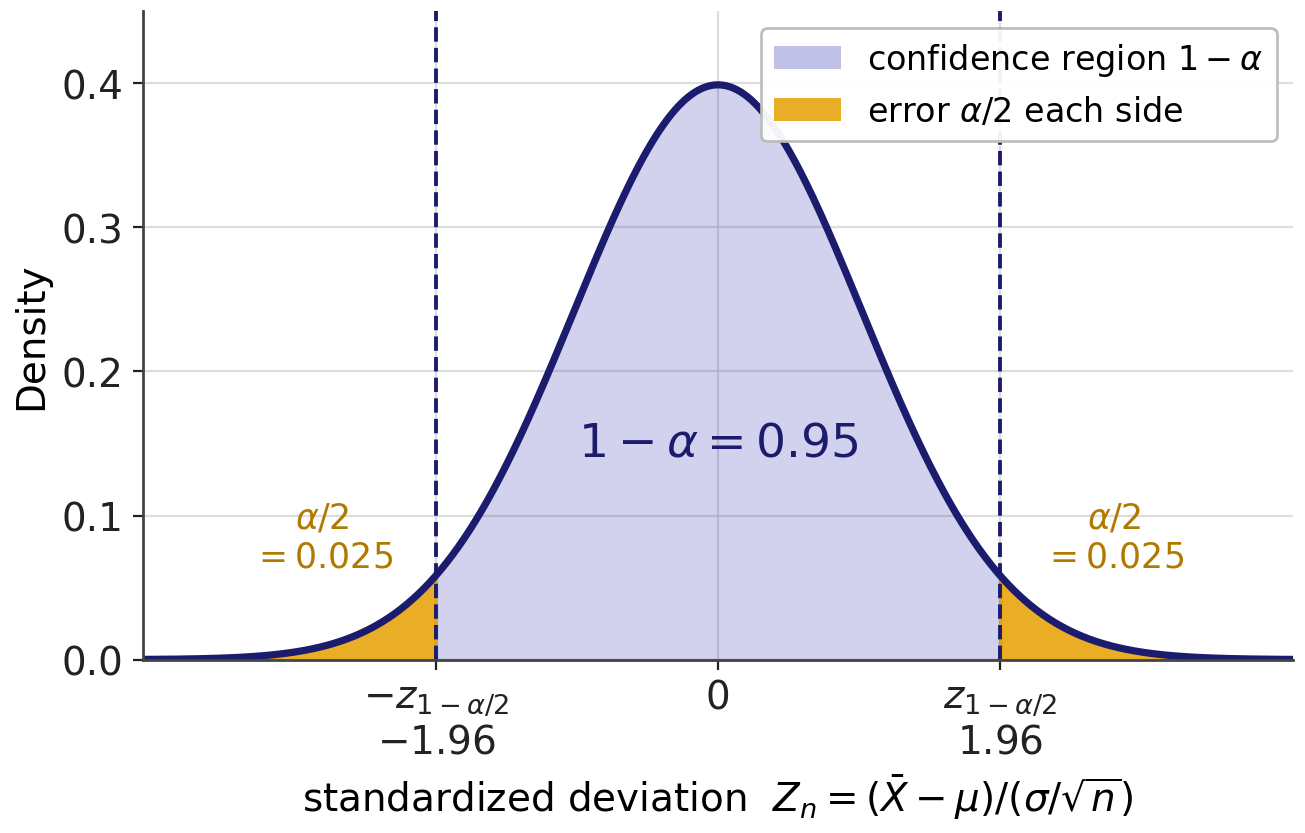
\includegraphics[width=0.80\textwidth,height=0.46\textheight,keepaspectratio]{images/mean_distribution.png}
  \end{center}
  \footnotesize The central (blue) region holds $95\,\%$ of the probability --
  in $95\,\%$ of samples $Z_n$ lands here; $2.5\,\%$ in each tail.
\end{frame}
\note{Talk track: no new theory here -- one sentence recalls the Foundations
(standard error, CLT), then the picture. Point at the blue area: ``95\,\% of
all samples land here.'' The next slide turns exactly this picture into a
probability statement, and the derivation turns that statement into the
confidence interval.}

% ---- How the mean fluctuates: formal statement -----------------------------
\begin{frame}{How does the mean fluctuate? -- formally}
  \begin{block}{Sampling distribution of the sample mean}
    For $X_i \sim N(\mu,\sigma^{2})$ i.i.d., the \emph{sampling distribution} of
    the random variable $\bar X$ is
    \[
      \bar{X} \sim N\!\left(\mu,\,\tfrac{\sigma^{2}}{n}\right)
      \quad\Longrightarrow\quad
      Z_n := \frac{\bar{X}-\mu}{\sigma/\sqrt{n}} \sim N(0,1).
    \]
  \end{block}
  {\footnotesize Both results are from the Foundations ($\mathrm{Var}(\bar X)=
  \sigma^2/n$, standardisation). New is the probability statement below -- the
  building block of the confidence interval.}
  \begin{block}{Two-sided probability statement}
    \[
      P\!\left(-z_{1-\alpha/2} \le Z_n \le z_{1-\alpha/2}\right) = 1-\alpha
    \]
  \end{block}
  \inworten{With probability $1-\alpha$, $Z_n$ lies between the two quantiles
  $\pm z_{1-\alpha/2}$.}
\end{frame}

% ---- Derivation ------------------------------------------------------------
\begin{frame}{Derivation (1/2): rearrange step by step}
  \footnotesize
  Start from the pivot $Z_n=\dfrac{\bar X-\mu}{\sigma/\sqrt n}\sim N(0,1)$, which lies
  within $\pm z_{1-\alpha/2}$ with probability $1-\alpha$:
  \begin{align*}
    1-\alpha
      &= P\!\left(-z_{1-\alpha/2}\ \le\ \tfrac{\bar X-\mu}{\sigma/\sqrt n}\ \le\ z_{1-\alpha/2}\right)
         && \rhd\ \text{\scriptsize starting point}\\[4pt]
      &= P\!\left(-z_{1-\alpha/2}\tfrac{\sigma}{\sqrt n}\ \le\ \bar X-\mu\ \le\ z_{1-\alpha/2}\tfrac{\sigma}{\sqrt n}\right)
         && \rhd\ \text{\scriptsize multiply all 3 parts by }\tfrac{\sigma}{\sqrt n}>0\\[4pt]
      &= P\!\left(-\bar X-z_{1-\alpha/2}\tfrac{\sigma}{\sqrt n}\ \le\ -\mu\ \le\ -\bar X+z_{1-\alpha/2}\tfrac{\sigma}{\sqrt n}\right)
         && \rhd\ \text{\scriptsize subtract }\bar X\text{ everywhere}
  \end{align*}
  \inworten{Multiplying by a \emph{positive} number keeps the ``$\le$'' signs; we
  only used equivalence steps, so the probability stays exactly $1-\alpha$.}
\end{frame}
\note{Talk track: the whole derivation is just ``solve the inequality for
$\mu$''. Announce that upfront so the algebra has a destination. Emphasise at
the end of (2/2): the randomness sits in the BOUNDS (they contain $\bar X$),
$\mu$ never moves -- that is what later justifies the careful CI
interpretation.}

\begin{frame}{Derivation (2/2): from $-\mu$ to the interval}
  \footnotesize
  \begin{align*}
    1-\alpha
      &= P\!\left(\bar X+z_{1-\alpha/2}\tfrac{\sigma}{\sqrt n}\ \ge\ \mu\ \ge\ \bar X-z_{1-\alpha/2}\tfrac{\sigma}{\sqrt n}\right)
         && \rhd\ \text{\scriptsize multiply by }(-1):\ \text{signs flip}\\[4pt]
      &= P\!\left(\bar X-z_{1-\alpha/2}\tfrac{\sigma}{\sqrt n}\ \le\ \mu\ \le\ \bar X+z_{1-\alpha/2}\tfrac{\sigma}{\sqrt n}\right)
         && \rhd\ \text{\scriptsize just read it left-to-right}
  \end{align*}
  \kernaussage{Confidence interval with \textbf{known} variance:
    \[
      \text{CI}_{1-\alpha} =
      \left[\bar{X}-z_{1-\alpha/2}\frac{\sigma}{\sqrt{n}},\;
            \bar{X}+z_{1-\alpha/2}\frac{\sigma}{\sqrt{n}}\right]
    \]}
  \footnotesize Multiplying an inequality by $-1$ \textbf{reverses} ``$\le$'' into
  ``$\ge$'' -- that is the only subtle step. What is random are the \emph{bounds}
  (they contain $\bar X$); $\mu$ itself is a fixed unknown.
\end{frame}

\begin{frame}{The formula in words}
  \[
    \text{CI} = \big[\;\underbrace{\bar{X}}_{\text{estimate}}
       \;\pm\; \underbrace{z_{1-\alpha/2}}_{\substack{\text{critical}\\\text{value}}}
       \cdot \underbrace{\tfrac{\sigma}{\sqrt{n}}}_{\text{standard error}}\;\big]
  \]
  \begin{itemize}\setlength{\itemsep}{4pt}
    \item \textbf{Centre} $\bar X$: our best estimate of $\mu$.
    \item \textbf{Standard error} $\sigma/\sqrt{n}$: how strongly $\bar X$
          fluctuates.
    \item \textbf{Critical value} $z_{1-\alpha/2}$: how many standard errors
          we go to the left/right ($1.96$ at $95\,\%$).
  \end{itemize}
\end{frame}

% ---- Milk calculation ------------------------------------------------------
\begin{frame}{Milk example: calculation}
  \textbf{Given:} $\bar{x}=1001$, $\sigma=3$, $n=9$, $\alpha=0.05$,
  $z_{0.975}=1.96$.
  \begin{align*}
    \text{margin of error } e &= z_{1-\alpha/2}\cdot\frac{\sigma}{\sqrt{n}}
       = 1.96\cdot\frac{3}{\sqrt{9}} = 1.96\\[2pt]
    \text{lower bound}  &= 1001 - 1.96 = 999.04\\
    \text{upper bound}  &= 1001 + 1.96 = 1002.96
  \end{align*}
  \begin{exampleblock}{Result}
    \[
      \text{CI}_{0.95} = \bigl[\,999.04\,;\,1002.96\,\bigr]\,\text{ml}
    \]
    The hypothesised target value $\mu_0 = 1000$ lies \emph{inside} the
    interval $\Rightarrow$ no evidence against a correctly working machine.
  \end{exampleblock}
\end{frame}

% ---- Exercise: filling cream, part 1 (known variance) ---------------------------
\begin{frame}{Exercise -- filling cream (known variance)}
  \begin{block}{Problem statement}
    A dairy fills cream into cups (label: $250\,\text{g}$). The variance of the
    machine is known: $\sigma^{2} = 4\,\text{g}^{2}$. After servicing, $n=16$
    cups are sampled (in g):
    \[
      251,248,248,249,250,251,247,246,252,251,248,247,246,249,248,252
    \]
    Confidence level $1-\alpha=0.95$.
  \end{block}
  \textbf{Required:} the confidence interval for $\mu$ with \emph{known}
  variance. Does the target value $250$\,g lie inside -- and what does that
  say about the machine?\\[2pt]
  \textbf{Hint:} $z_{0.975}=1.96$. (The same cups return with \emph{unknown}
  variance at the end of this section.)
\end{frame}

\begin{frame}{Solution -- filling cream (known variance)}
  \textbf{Rule:} $\text{CI}=\bigl[\bar x \pm z_{1-\alpha/2}\,\sigma/\sqrt{n}\bigr]$.\\[2pt]
  \textbf{Intermediate values:} $\bar{x} = 3983/16 = 248.9375$, $\sigma = 2$,
  $n = 16$, $z_{0.975} = 1.96$.
  \begin{align*}
    e &= 1.96\cdot\frac{2}{\sqrt{16}} = 1.96\cdot 0.5 = 0.98\\
    \text{CI}_{0.95} &= [\,248.9375 \pm 0.98\,]
       = \mathbf{[\,247.96\,;\,249.92\,]}
  \end{align*}
  \begin{alertblock}{Interpretation}
    The target value $\mu_0 = 250$ lies \emph{outside} the CI $\Rightarrow$ with
    known variance: indication that the machine is \textbf{not} working
    correctly.
  \end{alertblock}
\end{frame}

% ---- Interpretation: simulation -------------------------------------------
\begin{frame}{What does ``95\,\% confidence'' mean?}
  \begin{center}
    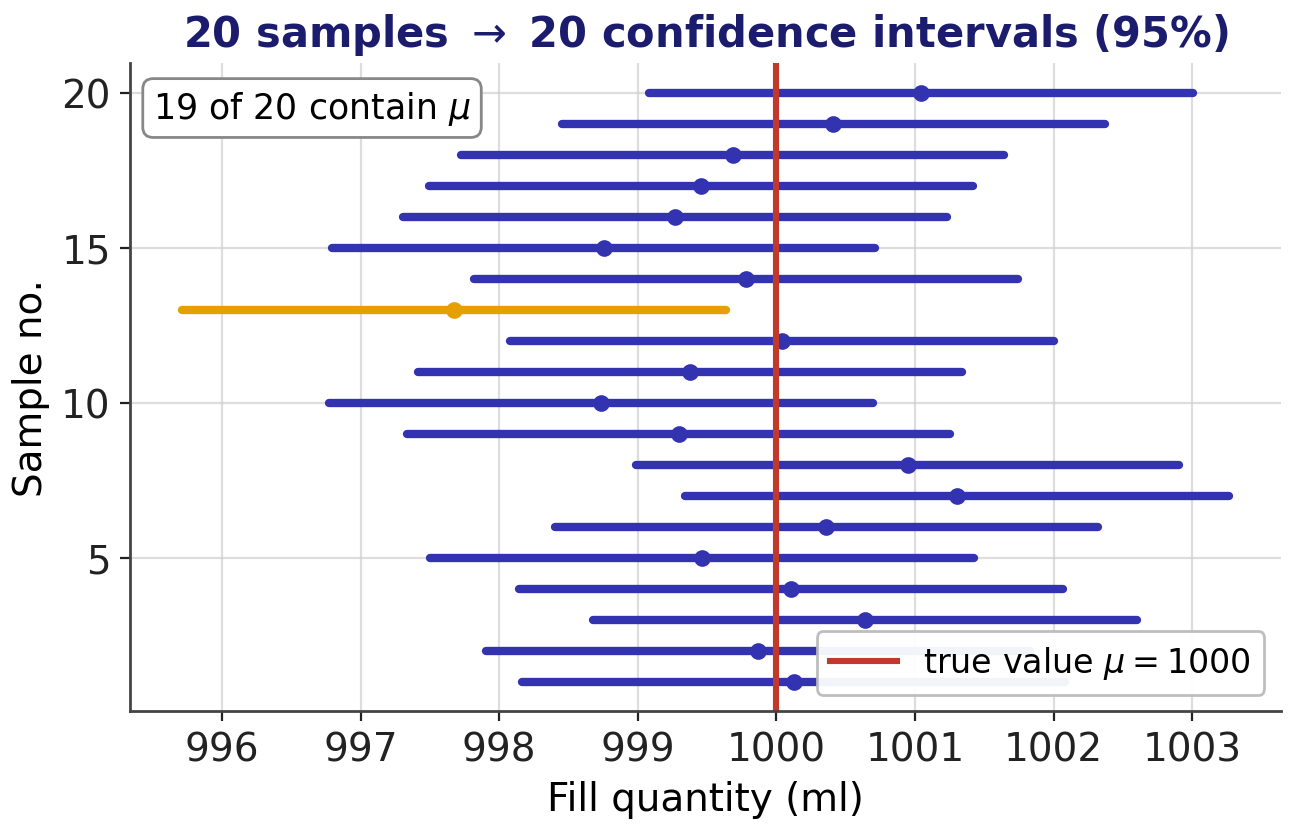
\includegraphics[width=0.80\textwidth,height=0.62\textheight,keepaspectratio]{images/ci_20_simulation.png}
  \end{center}
  \footnotesize Of $20$ computed $95\,\%$ intervals, on average $\approx 19$
  cover the true value $\mu$ (red line). The confidence \emph{level} refers to
  the \textbf{procedure} across many samples.
\end{frame}

% ---- Interpretation: misconception ----------------------------------------
\begin{frame}{A common misconception}
  \begin{alertblock}{Careful with the interpretation}
    ``With $95\,\%$ probability $\mu$ lies in \emph{this particular}
    interval'' is, strictly speaking, \textbf{wrong}.
  \end{alertblock}
  \begin{itemize}
    \item $\mu$ is a fixed (unknown) number -- it either is or is not inside
          the particular interval.
    \item What is random are the \emph{bounds} of the interval, not $\mu$.
    \item Correct: ``The \textbf{procedure} yields, in $95\,\%$ of samples, an
          interval that covers $\mu$.''
  \end{itemize}
\end{frame}

% ---- Interpretation: the correct readings ---------------------------------
\begin{frame}{Three correct ways to read a confidence interval}
  \begin{enumerate}\setlength{\itemsep}{5pt}
    \item \textbf{Coverage (the procedure).} The method produces intervals that
          contain the fixed true $\mu$ in a fraction $(1-\alpha)$ of all
          samples.
    \item \textbf{Compatibility.} The interval is the range of values for $\mu$
          that are \emph{consistent with the observed data}.
    \item \textbf{Duality with the test.} It is exactly the set of null values
          $\mu_0$ that a two-sided level-$\alpha$ test would \emph{not} reject.
  \end{enumerate}
  \kernaussage{All three avoid the trap of putting a probability on \emph{this
  one} interval: $\mu$ is fixed, the \textbf{interval} is what is random.}
\end{frame}

\begin{frame}{Do not confuse: CI vs.\ fluctuation interval}
  \begin{columns}[T]
    \begin{column}{0.60\textwidth}
      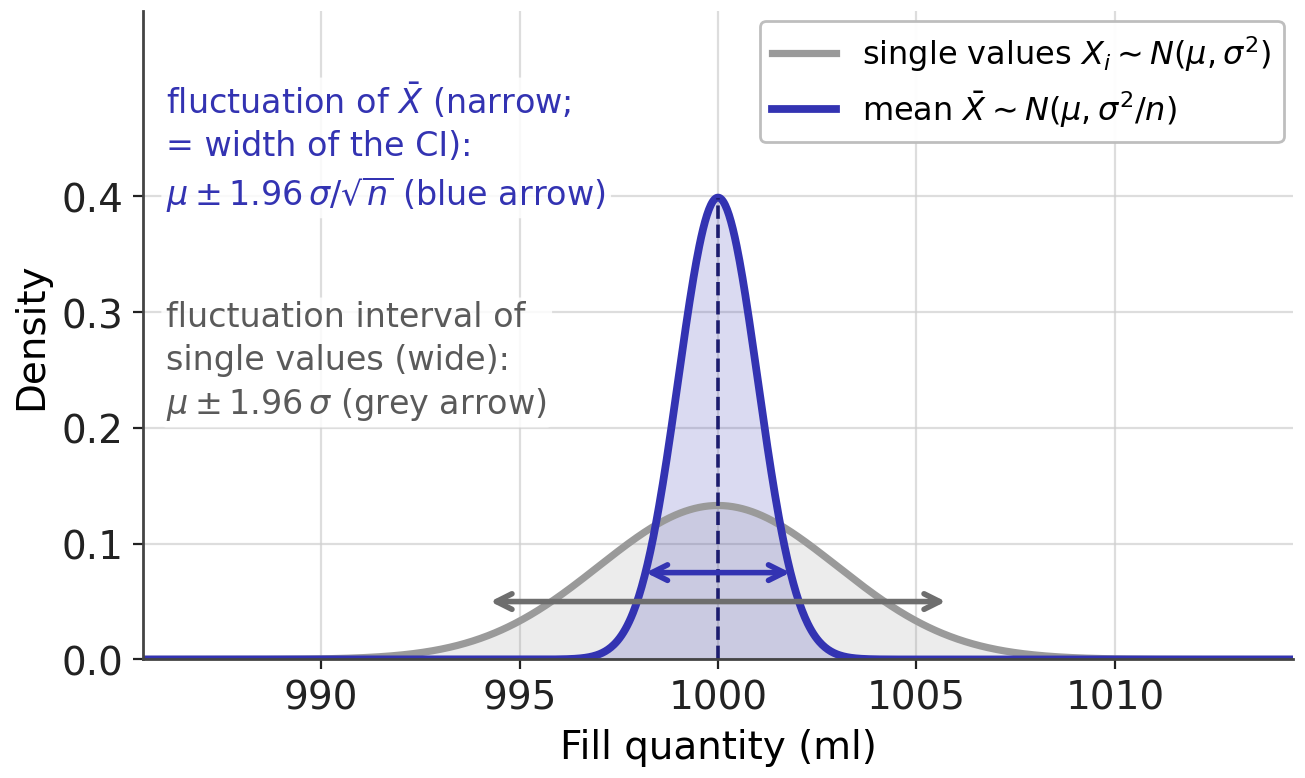
\includegraphics[width=\textwidth,height=0.64\textheight,keepaspectratio]{images/ci_vs_fluctuation.png}
    \end{column}
    \begin{column}{0.38\textwidth}
      \small
      \begin{itemize}\setlength{\itemsep}{5pt}
        \item \textbf{Fluctuation interval:} spread of \emph{individual} values
              $X_i$ around $\mu$ -- uses $\sigma$ (wide).
        \item \textbf{Confidence interval:} uncertainty about $\mu$ -- uses
              $\sigma/\sqrt{n}$ (narrow). It is exactly as wide as the
              fluctuation of $\bar X$ (blue arrow), but centred at $\bar x$,
              not at $\mu$.
      \end{itemize}
    \end{column}
  \end{columns}
  \inworten{Same width as the blue arrow, but a different question: ``Where is
  $\mu$?'' instead of ``How much does a single value scatter?''}
\end{frame}

% ---- Exercise: reading a CI correctly (SfOe Teil 6) ------------------------------
\begin{frame}{Exercise -- reading a confidence interval correctly}
  \begin{block}{Problem statement}
    For the cream sample ($n=16$, $\bar x=248.9375$\,g, $\sigma=2$\,g known)
    the $95\,\%$ CI $[\,247.96\,;\,249.92\,]$ was computed. Which of the
    following statements are \textbf{true}, which are \textbf{false}? Give a
    short reason.
  \end{block}
  \small
  \begin{enumerate}\setlength{\itemsep}{2pt}
    \item ``With $95\,\%$ probability the true mean $\mu$ lies between
          $247.96$\,g and $249.92$\,g.''
    \item ``About $95\,\%$ of all filled cups weigh between $247.96$\,g and
          $249.92$\,g.''
    \item ``If the sample were repeated very often, about $95\,\%$ of the
          intervals computed this way would contain the true value $\mu$.''
    \item ``The target value $250$\,g is \emph{not} compatible with the data
          at the $95\,\%$ level.''
    \item ``A $99\,\%$ interval from the same data would be \emph{narrower},
          because it is more certain.''
  \end{enumerate}
\end{frame}
\note{Talk track: let students vote true/false on each statement before
showing the solution. Statements 1 and 2 are the two classic misreadings
(probability of $\mu$; spread of single values); statement 5 tests the
confidence--precision trade-off. These formulations are typical
multiple-choice distractors.}

\begin{frame}{Solution (1/2) -- reading a confidence interval correctly}
  \textbf{Rule:} $\mu$ is a \emph{fixed} number; the \emph{bounds} are random.
  The confidence level describes the \emph{procedure}, not the one interval.
  \begin{exampleblock}{Answers 1--3}
    \begin{enumerate}\setlength{\itemsep}{3pt}
      \item \textbf{False.} $\mu$ either lies in this particular interval or it
            does not -- the probability $0.95$ belongs to the procedure across
            many samples.
      \item \textbf{False.} The CI describes the uncertainty about $\mu$
            (spread $\sigma/\sqrt n=0.5$), not the spread of single cups
            ($\sigma=2$). The fluctuation interval of the cups would be
            $248.9375\pm1.96\cdot2=\mathbf{[\,245.02\,;\,252.86\,]}$ -- four
            times as wide.
      \item \textbf{True.} That is exactly the coverage reading: the procedure
            hits $\mu$ in $95\,\%$ of the samples.
    \end{enumerate}
  \end{exampleblock}
\end{frame}

\begin{frame}{Solution (2/2) -- reading a confidence interval correctly}
  \begin{exampleblock}{Answers 4--5}
    \begin{enumerate}\setlength{\itemsep}{2pt}
      \setcounter{enumi}{3}
      \item \textbf{True.} $250\notin[\,247.96\,;\,249.92\,]$ -- the target is
            not among the values compatible with the data (``compatibility''
            reading). A two-sided test at level $5\,\%$ would reject
            $H_0:\mu=250$ (next section).
      \item \textbf{False.} More confidence costs precision:
            $z_{0.995}=2.576>1.96$, so $e=2.576\cdot\tfrac{2}{\sqrt{16}}=1.288$
            and $\text{CI}_{0.99}=[\,248.9375\pm1.288\,]
            =\mathbf{[\,247.65\,;\,250.23\,]}$ -- \emph{wider} than the
            $95\,\%$ CI, and now $250$ even lies \emph{inside}.
    \end{enumerate}
  \end{exampleblock}
  \kernaussage{A CI is a statement about the \textbf{procedure} and about the
  values of $\mu$ \textbf{compatible} with the data -- not about single values
  and not about ``the probability of $\mu$''.}
\end{frame}

\subsection{Length of the confidence interval}

\begin{frame}{What does the length depend on?}
  \begin{block}{Length}
    \[
      L = 2\cdot z_{1-\alpha/2}\cdot\frac{\sigma}{\sqrt{n}}
    \]
  \end{block}
  \begin{columns}[T]
    \begin{column}{0.48\textwidth}
      \begin{itemize}\setlength{\itemsep}{3pt}
        \item Higher confidence level $\Rightarrow$ larger
              $z_{1-\alpha/2}$ $\Rightarrow$ \emph{longer}.
        \item Larger $n$ $\Rightarrow$ \emph{shorter} (with $1/\sqrt{n}$).
        \item Larger spread $\sigma$ $\Rightarrow$ \emph{longer}.
      \end{itemize}
    \end{column}
    \begin{column}{0.48\textwidth}
      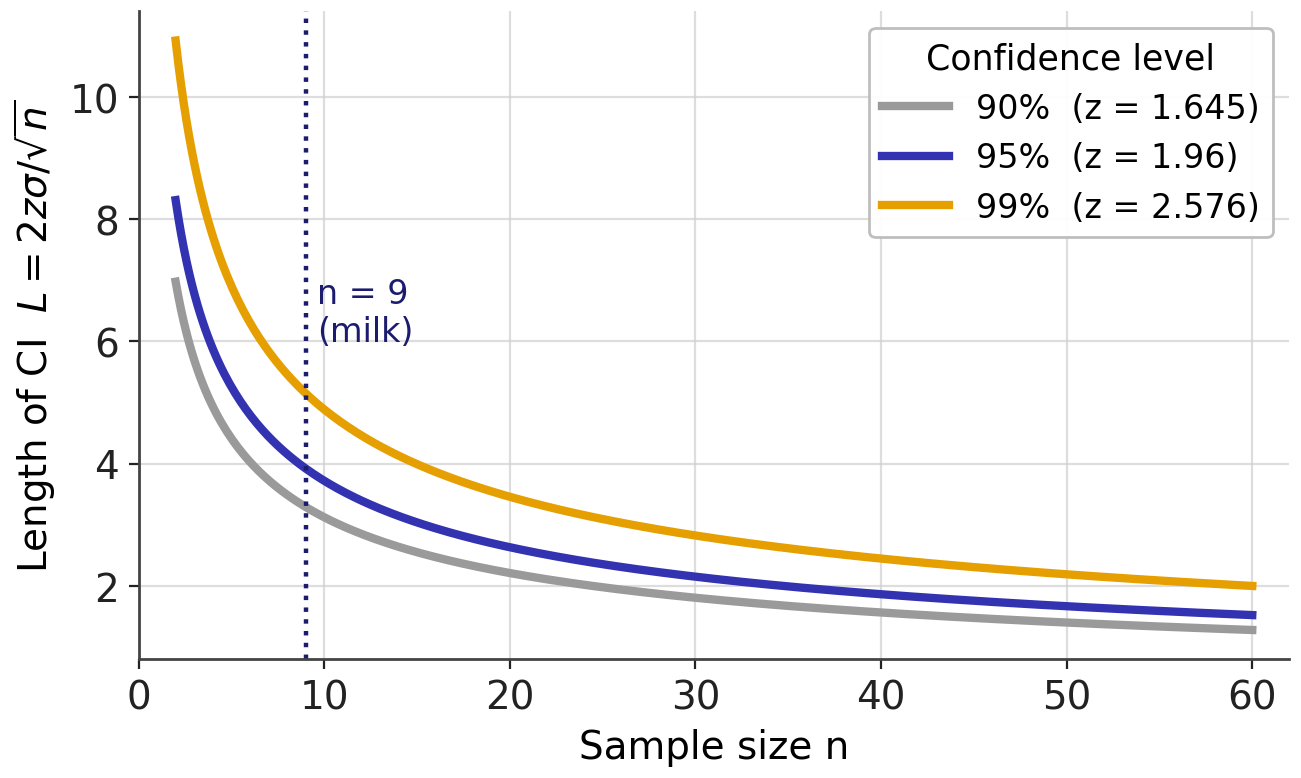
\includegraphics[width=\textwidth,height=0.48\textheight,keepaspectratio]{images/ci_length.png}
    \end{column}
  \end{columns}
  \inworten{More confidence \emph{or} more precision -- both require a larger
  sample.}
\end{frame}

\begin{frame}{Different confidence levels -- milk}
  \begin{center}
    \renewcommand{\arraystretch}{1.3}
    \begin{tabular}{lcc}
      \toprule
      Confidence level & Quantile $z_{1-\alpha/2}$ & CI for milk example \\
      \midrule
      $90\,\%$ & $z_{0.95}  = 1.645$ & $[999.36\,;\,1002.64]$\\
      $95\,\%$ & $z_{0.975} = 1.96$  & $[999.04\,;\,1002.96]$\\
      $99\,\%$ & $z_{0.995} = 2.576$ & $[998.42\,;\,1003.58]$\\
      \bottomrule
    \end{tabular}
  \end{center}
  \vspace{0.4em}
  \kernaussage{Higher confidence level $\Rightarrow$ wider interval
  $\Rightarrow$ less precise statement. Confidence and precision are a
  trade-off.}
\end{frame}

% ---- Planning the sample size ------------------------------------------------
\begin{frame}{Planning the sample size}
  \guidingquestion{How many bottles must the dairy measure so that the $95\,\%$
  CI is at most $\pm e$ wide -- e.g.\ $\pm1$\,ml?}
  \begin{block}{Solve the margin of error for $n$}
    \[
      e=z_{1-\alpha/2}\,\frac{\sigma}{\sqrt n}
      \quad\Longleftrightarrow\quad
      \sqrt n=\frac{z_{1-\alpha/2}\,\sigma}{e}
      \quad\Longrightarrow\quad
      n\ \ge\ \Bigl(\frac{z_{1-\alpha/2}\,\sigma}{e}\Bigr)^{2}
      \quad\text{(round \emph{up})}
    \]
  \end{block}
  \begin{itemize}\setlength{\itemsep}{2pt}
    \item $n$ grows with the \textbf{square} of $z\sigma/e$: halving the margin
          of error needs four times as many observations.
    \item Higher confidence (larger $z$) or a larger spread $\sigma$ also cost
          sample size.
    \item $\sigma$ unknown? Plan with an estimate from a pilot study or from
          past data.
  \end{itemize}
  \kernaussage{Decide on the precision you need \emph{before} collecting data
  -- the formula tells you what it costs.}
\end{frame}
\note{Talk track: this is the CI-length formula read backwards. Ask the room
first: ``we want half the margin -- twice the bottles?'' Most say yes; the
square says four times. Sample-size planning is the everyday business use of
this part (surveys, quality control, A/B tests); the same idea returns as
power analysis in the types-of-error section.}

% ---- Exercise: sample size (SfOe Teil 6) ------------------------------------------
\begin{frame}{Exercise -- how many bottles? (planning the sample size)}
  \begin{block}{Problem statement}
    The dairy (milk, $\sigma=3$\,ml known) wants to estimate the mean fill
    volume $\mu$ \emph{more precisely}. Quality control asks for a $95\,\%$ CI
    whose margin of error (half width) is at most $e=1$\,ml.
  \end{block}
  \begin{enumerate}\setlength{\itemsep}{2pt}
    \item[a)] What is the margin of error with the current sample ($n=9$)?
    \item[b)] At least how many bottles are needed for $e\le1$\,ml?
    \item[c)] How does $n$ change if the confidence level is to be $99\,\%$?
    \item[d)] How does $n$ change (at $95\,\%$) if the margin is halved to
              $e\le0.5$\,ml?
  \end{enumerate}
  \textbf{Hint:} $z_{0.975}=1.96$, $z_{0.995}=2.576$; always round $n$
  \emph{up}.
\end{frame}

\begin{frame}{Solution (1/2) -- planning the sample size}
  \textbf{Rule:} solve the margin of error $e=z_{1-\alpha/2}\,\sigma/\sqrt n$
  for $n$:
  \[
    n\ \ge\ \Bigl(\frac{z_{1-\alpha/2}\,\sigma}{e}\Bigr)^{2}
    \qquad\text{(round up to the next integer).}
  \]
  \begin{align*}
    \text{a)}\quad e &= 1.96\cdot\frac{3}{\sqrt9}=1.96\cdot1=\mathbf{1.96\ ml}
       \qquad(\text{the CI }[\,999.04\,;\,1002.96\,]\text{ from before})\\[4pt]
    \text{b)}\quad n &\ge \Bigl(\frac{1.96\cdot3}{1}\Bigr)^{2}=5.88^{2}=34.57
       \;\Longrightarrow\;\mathbf{n=35}\\[4pt]
    \text{c)}\quad n &\ge \Bigl(\frac{2.576\cdot3}{1}\Bigr)^{2}=7.728^{2}=59.72
       \;\Longrightarrow\;\mathbf{n=60}
  \end{align*}
  \inworten{b) For $\pm1$\,ml instead of $\pm1.96$\,ml the dairy needs almost
  four times as many bottles ($35$ instead of $9$). c) More confidence costs
  sample size ($60$ instead of $35$).}
\end{frame}

\begin{frame}[fragile]{Solution (2/2) -- planning the sample size}
  \[
    \text{d)}\quad n \ge \Bigl(\frac{1.96\cdot3}{0.5}\Bigr)^{2}=11.76^{2}=138.30
       \;\Longrightarrow\;\mathbf{n=139}
  \]
  \inworten{Half the margin $\Rightarrow$ four times the sample
  ($139\approx4\cdot35$): $n$ grows with the \textbf{square} of $z\sigma/e$.}
  \par\smallskip
  {\small The same with Python:\par}
\begin{lstlisting}
import math
from scipy import stats
def n_required(conf, sigma, e):
    z = stats.norm.ppf(1 - (1 - conf) / 2)
    return math.ceil((z * sigma / e) ** 2)
print(n_required(0.95, 3, 1), n_required(0.99, 3, 1), n_required(0.95, 3, 0.5))
\end{lstlisting}
  \begin{block}{Output}
\begin{lstlisting}[style=Pyout]
35 60 139
\end{lstlisting}
  \end{block}
  \trynotebook{section 2.3 ``Length of the confidence interval''}
\end{frame}

\subsection{Unknown variance}

% ---- Problem & t-distribution ----------------------------------------------
\begin{frame}{More realistic: the variance is unknown}
  \begin{block}{Problem}
    In practice $\sigma^{2}$ is almost never known. We must \emph{also
    estimate} it from the sample.
  \end{block}
  \begin{block}{Estimator of the variance}
    \[
      s^{2} = \frac{1}{n-1}\sum_{i=1}^{n}(X_i - \bar{X})^{2}
    \]
  \end{block}
  \begin{itemize}
    \item We replace $\sigma$ by $s$ in the test statistic.
    \item This costs \emph{accuracy} -- and changes the distribution
          (see next slide).
  \end{itemize}
\end{frame}

\begin{frame}{Why the $t$-distribution? -- intuitively and graphically}
  \begin{columns}[T]
    \begin{column}{0.46\textwidth}
      \begin{block}{Standardised statistic (normal data)}
        \[
          T_n = \frac{\bar{X}-\mu}{s/\sqrt{n}} \sim t_{n-1}
        \]
      \end{block}
      \begin{itemize}\setlength{\itemsep}{2pt}
        \item $s$ is \textbf{itself a random variable}.
        \item $T_n$ is a ratio of \emph{two} random quantities $\Rightarrow$
              \textbf{heavier tails}.
        \item For large $n$, $s$ barely varies, so $t_{n-1}\to N(0,1)$.
      \end{itemize}
    \end{column}
    \begin{column}{0.52\textwidth}
      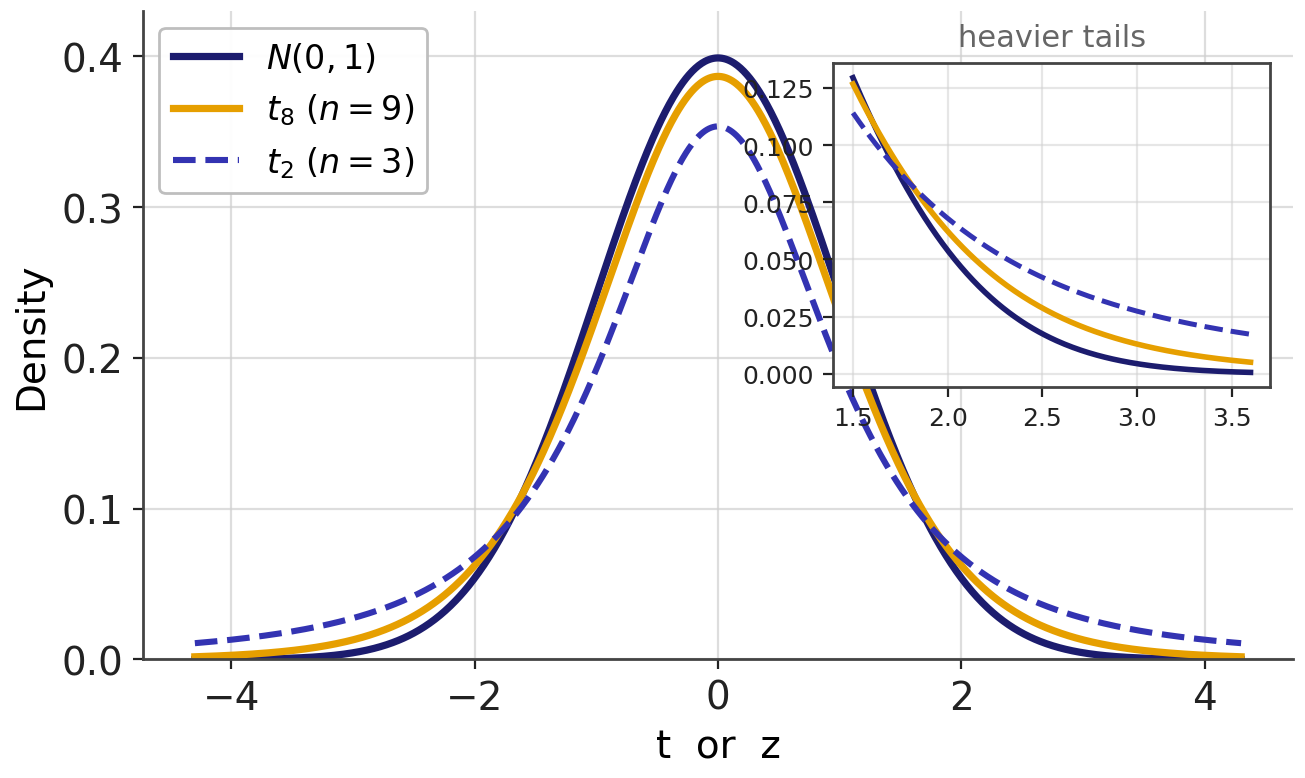
\includegraphics[width=\textwidth,height=0.50\textheight,keepaspectratio]{images/t_vs_normal.png}
    \end{column}
  \end{columns}
  \kernaussage{Unknown $\sigma$ $\Rightarrow$ use $t_{n-1}$: larger quantiles,
  so the CI is wider on average.}
\end{frame}

\begin{frame}{Milk example with unknown variance}
  \begin{block}{Confidence interval}
    \[
      \text{CI} = \left[\bar{X} - t_{1-\alpha/2,\,n-1}\frac{s}{\sqrt{n}},\;
                         \bar{X} + t_{1-\alpha/2,\,n-1}\frac{s}{\sqrt{n}}\right]
    \]
  \end{block}
  \textbf{Data:} $\bar{x}=1001$, $n=9$, $\alpha=0.05$, $s = 3.7749$,
  $t_{0.975;\,8} = 2.3060$.
  \begin{align*}
    e &= 2.3060\cdot\frac{3.7749}{\sqrt{9}} = 2.9017\\
    \text{CI}_{0.95} &= [\,1001\pm 2.9017\,] = [\,998.10\,;\,1003.90\,]
  \end{align*}
  \begin{exampleblock}{Comparison}
    Wider than $[999.04\,;\,1002.96]$ (known variance) -- the price for
    estimating $\sigma$.
  \end{exampleblock}
\end{frame}

\begin{frame}{Summary: known vs.\ unknown variance}
  \begin{center}
    \renewcommand{\arraystretch}{1.3}
    \begin{tabular}{lcc}
      \toprule
       & \textbf{known} $\sigma$ & \textbf{unknown} $\sigma$\\
      \midrule
      Spread used      & $\sigma$ & $s$ (estimated)\\
      Distribution     & $N(0,1)$ & $t_{n-1}$\\
      Quantile ($95\,\%$, $n=9$) & $1.96$ & $2.31$\\
      CI               & narrower & wider (on average)\\
      \bottomrule
    \end{tabular}
  \end{center}
  \begin{itemize}
    \item For large $n$ ($n \gtrsim 30$) the difference is small
          ($t_{n-1}\approx N(0,1)$).
    \item For small samples it is clearly noticeable.
  \end{itemize}
\end{frame}

% ---- Confidence intervals with Python -------------------------------------------
\begin{frame}[fragile]{Confidence intervals with Python}
\begin{lstlisting}
import numpy as np
from scipy import stats
milk = np.array([1005, 1001, 997, 1000, 1001, 998, 999, 999, 1009])
xbar, n, s = milk.mean(), len(milk), milk.std(ddof=1)    # 1001.0, 9, 3.7749
stats.norm.ppf(0.975), stats.t.ppf(0.975, df=n - 1)     # quantiles: 1.9600, 2.3060
for conf in (0.90, 0.95, 0.99):                          # sigma = 3 known -> N(0,1)
    lo, hi = stats.norm.interval(conf, loc=xbar, scale=3 / np.sqrt(n))
    print(f"z, {conf:.0%}: [{lo:.2f}, {hi:.2f}]")
lo, hi = stats.t.interval(0.95, df=n - 1, loc=xbar, scale=s / np.sqrt(n))
print(f"t, 95%: [{lo:.2f}, {hi:.2f}]")                   # sigma estimated -> t_(n-1)
\end{lstlisting}
  \begin{columns}[T]
    \begin{column}{0.42\textwidth}
      \begin{block}{Output}
\begin{lstlisting}[style=Pyout]
z, 90%: [999.36, 1002.64]
z, 95%: [999.04, 1002.96]
z, 99%: [998.42, 1003.58]
t, 95%: [998.10, 1003.90]
\end{lstlisting}
      \end{block}
    \end{column}
    \begin{column}{0.54\textwidth}
      \footnotesize \texttt{interval(conf, ...)} $=$ $\bar x\pm$ quantile
      $\cdot$ SE: \texttt{loc} $=\bar x$, \texttt{scale} $=$ standard error
      ($\sigma/\sqrt n$ or $s/\sqrt n$), for $t$ also \texttt{df} $=n-1$.
      Same numbers as on the milk slides.
    \end{column}
  \end{columns}
  \trynotebook{section 2.4 ``Unknown variance''}
\end{frame}

% ---- Exercise: filling cream, part 2 (unknown variance) -------------------------
\begin{frame}{Exercise -- filling cream (unknown variance)}
  \begin{block}{Problem statement}
    The same $16$ cream cups as in the known-variance exercise (label
    $250\,\text{g}$, in g):
    \[
      251,248,248,249,250,251,247,246,252,251,248,247,246,249,248,252
    \]
    This time we do \emph{not} rely on the stated machine variance but
    estimate $\sigma$ from the sample. Confidence level $1-\alpha=0.95$.
  \end{block}
  \textbf{Required:} the sample standard deviation $s$ and the confidence
  interval for $\mu$ with \emph{unknown} variance. Does the verdict on
  $250$\,g change compared with $[\,247.96\,;\,249.92\,]$ (known variance)?\\[2pt]
  \textbf{Hint:} $\bar x=248.9375$, \
  $\sum_{i}(x_i-\bar x)^2=60.9375$, \ $t_{0.975;\,15}=2.1314$.
\end{frame}

\begin{frame}{Solution -- filling cream (unknown variance)}
  \textbf{Rule:} as for known variance, but $z\to t_{1-\alpha/2,\,n-1}$ and
  $\sigma\to s$.\\[2pt]
  \textbf{Intermediate values:} $s^{2} = 60.9375/15 = 4.0625\Rightarrow
  s = 2.0156$, $t_{0.975;\,15} = 2.1314$.
  \begin{align*}
    e &= 2.1314\cdot\frac{2.0156}{\sqrt{16}} = 1.0740\\
    \text{CI}_{0.95} &= [\,248.9375 \pm 1.0740\,]
       = \mathbf{[\,247.86\,;\,250.01\,]}
  \end{align*}
  \begin{exampleblock}{Comparison}
    Now $\mu_0 = 250$ lies (just) \emph{inside} the CI -- the verdict turns out
    \emph{differently} than with known variance. The wider $t$-interval is more
    cautious.
  \end{exampleblock}
\end{frame}

\begin{frame}{Summary and outlook}
  \begin{itemize}\setlength{\itemsep}{4pt}
    \item Confidence intervals quantify the \textbf{uncertainty} of a point
          estimate.
    \item Known variance: quantiles of $N(0,1)$; unknown: of $t_{n-1}$.
    \item The required precision fixes the \textbf{sample size}:
          $n\ge(z_{1-\alpha/2}\,\sigma/e)^2$.
    \item \textbf{Bridge to the test:} if the CI contains the hypothesised
          value $\mu_0$, there is no evidence against $H_0:\mu=\mu_0$ --
          otherwise there is.
  \end{itemize}
  \begin{block}{Next section}
    We formalise this procedure as a \textbf{hypothesis test}.
  \end{block}
\end{frame}
% ============================================================================
% SECTION 3: HYPOTHESIS TESTS
% ============================================================================
\section[Tests]{Hypothesis Tests}

\subsection{Idea and hypotheses}

% ---- Intuition: courtroom --------------------------------------------------
\begin{frame}{What is a hypothesis test? -- intuition}
  \begin{block}{The basic idea, as in court}
    An assumption (the \emph{null hypothesis} $H_0$) is held true until the
    data \textbf{speak strongly enough against it}.
  \end{block}
  \begin{columns}[T]
    \begin{column}{0.48\textwidth}
      \begin{itemize}\setlength{\itemsep}{3pt}
        \item \textbf{$H_0$} = ``innocent'' (status quo).
        \item We reject $H_0$ only on \emph{convincing} evidence.
        \item Little evidence $\Rightarrow$ acquittal for lack of evidence
              -- not ``proven innocent''.
      \end{itemize}
    \end{column}
    \begin{column}{0.48\textwidth}
      \begin{exampleblock}{Milk}
        $H_0:\mu = 1000$ -- ``the machine works correctly''.
        Only a clear deviation from $1000$ makes us doubt this.
      \end{exampleblock}
    \end{column}
  \end{columns}
\end{frame}

% ---- Hypotheses & asymmetry ------------------------------------------------
\begin{frame}{The two hypotheses}
  \begin{block}{Structure}
    \[
      H_0:\mu = \mu_0 \qquad\text{vs.}\qquad H_1:\mu \neq \mu_0
    \]
  \end{block}
  \begin{itemize}\setlength{\itemsep}{3pt}
    \item We \textbf{always} argue under ``$H_0$ is true''.
    \item Why unequal? $H_0:\mu=\mu_0$ fixes a \emph{single} value, so the test
          statistic has \emph{one} definite distribution we can compute with;
          $H_1$ is a whole \emph{range}, with no single distribution.
    \item Two outcomes: \emph{keep} $H_0$ or \emph{reject} it.
  \end{itemize}
  \kernaussage{What you want to \textbf{establish} statistically goes into
  $H_1$.}
\end{frame}

\begin{frame}{Which hypothesis goes where?}
  \begin{block}{Rule of thumb}
    The statement you want to \emph{find evidence for} -- the ``more
    important'' claim -- is formulated as $H_1$, because only the Type~I error
    (wrongly rejecting $H_0$) can be controlled via $\alpha$.
  \end{block}
  \vspace{0.4em}
  \begin{center}
    \renewcommand{\arraystretch}{1.5}
    \begin{tabular}{@{}p{8.2cm}cc@{}}
      \toprule
      \textbf{You want evidence that \ldots} & \textbf{$H_0$} & \textbf{$H_1$}\\
      \midrule
      the supplier's fill weight \emph{deviates} from the spec
        & $\mu = \mu_0$ & $\mu \neq \mu_0$\\
      the mean processing time \emph{changed} after the update
        & $\mu = \mu_0$ & $\mu \neq \mu_0$\\
      the mean daily revenue \emph{differs} from the plan figure
        & $\mu = \mu_0$ & $\mu \neq \mu_0$\\
      \bottomrule
    \end{tabular}
  \end{center}
\end{frame}

\subsection{From CI to test}

% ---- CI <-> test equivalence -----------------------------------------------
\begin{frame}{Bridge: confidence interval and test are the same}
  \begin{block}{Testing with the CI}
    If $\mu_0$ lies \emph{inside} the confidence interval, $H_0:\mu=\mu_0$ is
    \textbf{not} rejected -- if it lies outside, it is.
  \end{block}
  \begin{block}{Equivalence -- same algebra, two readings}
    ``$\mu_0$ inside the CI'' means
    $|\bar x-\mu_0|\le z_{1-\alpha/2}\,\sigma/\sqrt n$, which rearranges to
    $|Z_n|\le z_{1-\alpha/2}$ -- exactly the non-rejection condition. So a
    test (level $\alpha$) and a CI (level $1-\alpha$) \textbf{always} agree.
  \end{block}
  \inworten{The CI shows \emph{all} $\mu_0$ that you would not reject.}
\end{frame}

% ---- Duality on the number line (both running examples) --------------------
\begin{frame}{The duality on the number line}
  \centering
  {\small\textbf{Milk:} $\mu_0=1000$ lies \emph{inside} the CI
   $\Rightarrow$ \textcolor{hsbiblaudunkel}{\textbf{keep $H_0$}}}\\[4pt]
  \begin{tikzpicture}[x=1.30cm]
    \draw[->,thick,gray] (-0.2,0) -- (6.6,0) node[right,font=\scriptsize,black]{ml};
    \draw[line width=5pt, hsbiblau!55] (1.04,0) -- (4.96,0);
    \node[above,font=\scriptsize,hsbiblau] at (4.35,0.10) {$95\,\%$ CI};
    \fill[hsbiblaudunkel] (3,0) circle (2.2pt)
      node[above=3pt,font=\scriptsize]{$\bar x=1001$};
    \draw[very thick, hsbirot] (2,0.16)--(2,-0.16)
      node[below=7pt,font=\scriptsize,hsbirot]{$\mu_0=1000$};
    \node[below=1pt,font=\scriptsize,hsbiblau] at (1.04,0) {$999.04$};
    \node[below=1pt,font=\scriptsize,hsbiblau] at (4.96,0) {$1002.96$};
  \end{tikzpicture}\\[10pt]
  {\small\textbf{Cream:} $\mu_0=250$ lies \emph{outside} the CI
   $\Rightarrow$ \textcolor{hsbirot}{\textbf{reject $H_0$}}}\\[4pt]
  \begin{tikzpicture}[x=1.95cm]
    \draw[->,thick,gray] (-0.2,0) -- (3.7,0) node[right,font=\scriptsize,black]{g};
    \draw[line width=5pt, hsbiblau!55] (0.96,0) -- (2.92,0);
    \fill[hsbiblaudunkel] (1.94,0) circle (2.2pt)
      node[above=3pt,font=\scriptsize]{$\bar x=248.94$};
    \draw[very thick, hsbirot] (3.0,0.16)--(3.0,-0.16)
      node[below right=7pt and -6pt,font=\scriptsize,hsbirot]{$\mu_0=250$};
    \node[below=1pt,font=\scriptsize,hsbiblau] at (0.96,0) {$247.96$};
    \node[below left=1pt and -4pt,font=\scriptsize,hsbiblau] at (2.92,0) {$249.92$};
  \end{tikzpicture}
  \kernaussage{$\mu_0$ inside the CI $\Leftrightarrow$ keep $H_0$;\quad
  outside $\Leftrightarrow$ reject. (Both at known $\sigma$, $\alpha=0.05$.)}
\end{frame}
\note{Talk track: ``the CI is the set of all null values that survive the
test.'' Walk both lines: milk -- target inside, nothing to complain about;
cream -- target outside, the data are incompatible with 250\,g. Point out the
CI is centred at $\bar x$, never at $\mu_0$.}

% ---- Graphic: same figure, two readings ------------------------------------
\begin{frame}{One picture, two readings}
  \begin{columns}[T]
    \begin{column}{0.58\textwidth}
      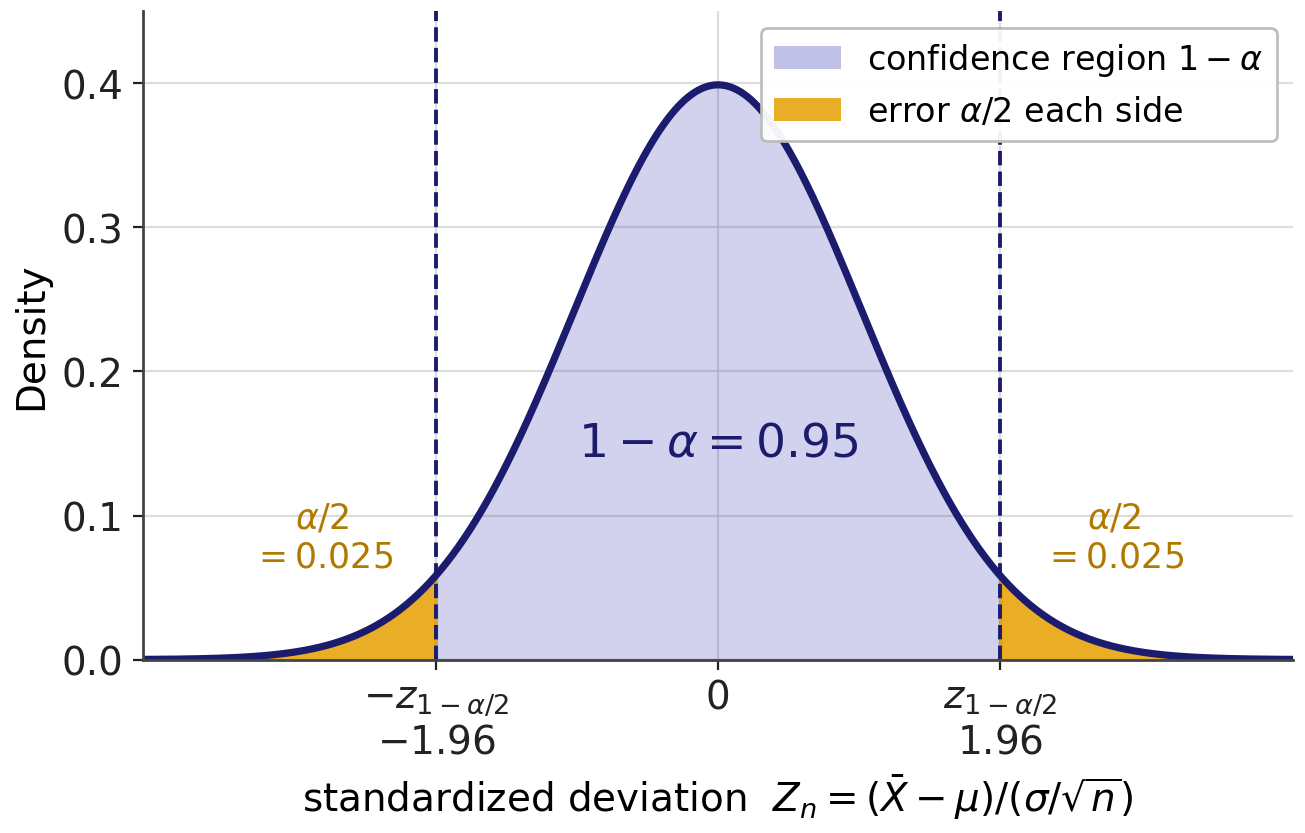
\includegraphics[width=\textwidth,height=0.62\textheight,keepaspectratio]{images/mean_distribution.png}
    \end{column}
    \begin{column}{0.40\textwidth}
      \footnotesize
      \begin{itemize}\setlength{\itemsep}{5pt}
        \item \textbf{Distribution reading:} the central blue region holds
              $95\,\%$ of the $Z_n$ distribution (in $95\,\%$ of samples $Z_n$
              lands here).
        \item \textbf{Test reading:} blue = \textbf{acceptance region}
              ($=$ non-rejection region), orange = \textbf{rejection region}
              ($\alpha$).
        \item Test statistic in the orange tail $\Rightarrow$ reject $H_0$.
      \end{itemize}
      \vspace{2pt}``Acceptance region'' is conventional for the
      \emph{non-rejection} region: landing there means we \emph{fail to reject}
      $H_0$, not that we accept it as true.
    \end{column}
  \end{columns}
\end{frame}

% ---- Quick exercise: hypotheses + duality (SfOe Teil 6) --------------------------
\begin{frame}{Exercise -- hypotheses and deciding with the CI}
  \begin{block}{Problem statement}
    A bank plans its staff with a mean processing time of $\mu_0=30$\,min per
    loan application. Longer times (bottlenecks) and shorter times
    (overcapacity) matter equally. From experience $\sigma=6$\,min is known. A
    sample of $n=36$ applications gives $\bar x=32.8$\,min; \ $\alpha=0.05$.
  \end{block}
  \begin{enumerate}\setlength{\itemsep}{3pt}
    \item[a)] State $H_0$ and $H_1$.
    \item[b)] Compute the $95\,\%$ CI for $\mu$.
    \item[c)] Decide about $H_0$ with the CI.
    \item[d)] Which of the planning values $\mu_0=31$, $33$ and $35$\,min would
              a two-sided test at level $5\,\%$ reject?
  \end{enumerate}
  \textbf{Hint:} $z_{0.975}=1.96$.
\end{frame}
\note{Talk track: four minutes. Part a) practises ``the deviation you want to
detect goes into $H_1$''; part d) is the payoff of the duality -- one interval
answers the test for every $\mu_0$ at a glance, without a single new
calculation.}

\begin{frame}{Solution -- hypotheses and deciding with the CI}
  \textbf{Rule:} $\mu_0$ inside the $(1-\alpha)$-CI $\Leftrightarrow$
  $|Z_n|\le z_{1-\alpha/2}$ $\Leftrightarrow$ keep $H_0$.
  \begin{itemize}\setlength{\itemsep}{4pt}
    \item[a)] $H_0:\mu=30$ \ vs.\ \ $H_1:\mu\neq30$ -- both directions count;
          the deviation to be detected goes into $H_1$.
    \item[b)] $\mathrm{SE}=6/\sqrt{36}=6/6=1$, \ $e=1.96\cdot1=1.96$, \
          $\text{CI}_{0.95}=[\,32.8\pm1.96\,]=\mathbf{[\,30.84\,;\,34.76\,]}$\,min.
    \item[c)] $30\notin\text{CI}$ $\Rightarrow$ $H_0$ is \textbf{rejected}: the
          mean processing time deviates from the planning value. (Cross-check:
          $|Z_n|=|32.8-30|/1=2.8>1.96$.)
    \item[d)] One look at the CI suffices: $31$ and $33$ lie inside
          $[\,30.84\,;\,34.76\,]$ $\Rightarrow$ \textbf{keep}; \ $35$ lies
          outside $\Rightarrow$ \textbf{reject}.
  \end{itemize}
  \kernaussage{A CI answers the two-sided test for \emph{every} hypothesised
  value $\mu_0$ at once.}
\end{frame}

\subsection{Known variance}

% ---- Critical value intuition (moved here: used by the recipe below) -------
\begin{frame}{The critical value -- the bar you must clear}
  \begin{block}{Plain idea}
    The \textbf{critical value} is a fixed threshold on the test statistic. It
    splits all possible outcomes into two zones:
  \end{block}
  \begin{columns}[T]
    \begin{column}{0.48\textwidth}
      \begin{exampleblock}{Keep $H_0$}
        Statistic \emph{inside} the threshold -- the deviation is small enough
        to pass as ordinary chance.
      \end{exampleblock}
    \end{column}
    \begin{column}{0.48\textwidth}
      \begin{alertblock}{Reject $H_0$}
        Statistic \emph{beyond} the threshold -- too extreme to be chance at
        level $\alpha$.
      \end{alertblock}
    \end{column}
  \end{columns}
\end{frame}
\note{Talk track: ``A critical value is just a line in the sand on the test
statistic.'' Use the high-jump image -- $\alpha$ sets the bar height; smaller
$\alpha$ = higher bar = harder to reject. Common student confusion: thinking a
larger statistic is automatically ``better'' -- it only matters relative to the
bar. Anchor: the acceptance region is everything inside the bar(s).}

% ---- Recipe (TikZ flow) ----------------------------------------------------
\begin{frame}{The test recipe (known variance)}
  \centering
  \resizebox{\textwidth}{!}{%
  \begin{tikzpicture}[node distance=6mm]
    \node[flowbox, text width=2.5cm] (h)
      {\footnotesize \textbf{1. Hypotheses}\\ $H_0:\mu=\mu_0$\\ $H_1:\mu\neq\mu_0$};
    \node[flowbox, text width=2.7cm, right=8mm of h] (z)
      {\footnotesize \textbf{2. Test statistic}\\ $Z_n=\dfrac{\bar x-\mu_0}{\sigma/\sqrt n}$};
    \node[flowbox, text width=2.5cm, right=8mm of z] (c)
      {\footnotesize \textbf{3. Critical value}\\ $z_{1-\alpha/2}$};
    \node[diamond, draw=hsbiblaudunkel, very thick, fill=hsbiblau!8,
          aspect=2, inner sep=1pt, text width=2.2cm, align=center,
          right=8mm of c] (d) {\scriptsize $|Z_n|>z_{1-\alpha/2}$?};
    \node[flowboxo, text width=2.3cm, above right=2mm and 8mm of d] (ja)
      {\footnotesize \textbf{yes:} reject $H_0$};
    \node[flowboxg, text width=2.3cm, below right=2mm and 8mm of d] (nein)
      {\footnotesize \textbf{no:} keep $H_0$};
    \draw[flowarr] (h)--(z); \draw[flowarr] (z)--(c); \draw[flowarr] (c)--(d);
    \draw[flowarr] (d.north) to[out=90,in=180] (ja.west);
    \draw[flowarr] (d.south) to[out=-90,in=180] (nein.west);
  \end{tikzpicture}}
  \vspace{0.8em}
  \begin{itemize}
    \item \textbf{Key move:} plug the hypothesised $\mu_0$ in for the unknown
          $\mu$ (the same $Z_n$ as for the CI, only with $\mu_0$ instead of
          $\mu$) -- \emph{if} $H_0$ holds then $Z_n\sim N(0,1)$, so a $|Z_n|$
          that would be very unusual for $N(0,1)$ is evidence against $H_0$.
    \item $|Z_n|\le z_{1-\alpha/2}$: acceptance (non-rejection) region; beyond
          it: rejection region (area $\alpha$ under $H_0$). Fix $\alpha$
          \emph{in advance}.
  \end{itemize}
\end{frame}

\begin{frame}{Milk test with known variance}
  \textbf{Data:} $\bar{x}=1001$, $\sigma=3$, $n=9$, $\mu_0=1000$,
  $\alpha=0.05$, $z_{0.975}=1.96$.
  \begin{align*}
    Z_n &= \frac{1001-1000}{3/\sqrt{9}} = \frac{1}{1} = 1.000\\[2pt]
    |Z_n| &= 1.000 \;<\; 1.96 = z_{0.975}
  \end{align*}
  \begin{exampleblock}{Decision}
    $H_0:\mu=1000$ is \textbf{not} rejected -- no evidence against a correctly
    working machine.
  \end{exampleblock}
  \inworten{Same result as the CI: $\mu_0=1000 \in [999.04\,;\,1002.96]$.}
\end{frame}

\subsection{Unknown variance}

\begin{frame}{Test with unknown variance}
  \begin{block}{Only two changes to the recipe}
    \[
      T_n = \frac{\bar{X}-\mu_0}{s/\sqrt{n}} \sim t_{n-1}\ \text{under } H_0,
      \qquad
      \text{rejection: } |T_n| > t_{1-\alpha/2,\,n-1}.
    \]
  \end{block}
  \begin{itemize}
    \item $\sigma \to s$ (estimated) and $z \to t_{n-1}$.
    \item \textbf{Assumption:} data (approximately) normally distributed
          \emph{or} $n \ge 30$ (central limit theorem).
  \end{itemize}
\end{frame}

\begin{frame}{Milk test with unknown variance}
  \textbf{Data:} $\bar{x}=1001$, $s=3.7749$, $n=9$, $\mu_0=1000$,
  $\alpha=0.05$, $t_{0.975;\,8}=2.3060$.
  \begin{align*}
    T_n &= \frac{1001-1000}{3.7749/\sqrt{9}} = \frac{1}{1.2583} = 0.7947\\[2pt]
    |T_n| &= 0.7947 \;<\; 2.3060 = t_{0.975;\,8}
  \end{align*}
  \begin{exampleblock}{Decision}
    $H_0:\mu=1000$ is \textbf{not} rejected. (More cautious $t$-quantile
    $2.31$ instead of $1.96$ -- the result is nevertheless the same here.)
  \end{exampleblock}
\end{frame}

% ---- Assumptions checklist ---------------------------------------------------
\begin{frame}{Before you test -- the assumptions checklist}
  \begin{enumerate}\setlength{\itemsep}{5pt}
    \item \textbf{Random sample, independent observations} -- the $X_i$ are
          i.i.d.\ draws from the population. (No clustering, no repeated
          measurements of the same unit.)
    \item \textbf{Distribution:} data approximately normal \emph{or}
          $n\gtrsim 30$ -- then the CLT (Foundations) makes $\bar X$
          approximately normal.
    \item \textbf{Spread:} $\sigma$ known $\to$ $z$-test; \ $\sigma$ estimated
          by $s$ $\to$ $t$-test with $\mathrm{df}=n-1$.
    \item \textbf{Question fixed in advance:} $\mu_0$, the direction
          (one-/two-sided) and $\alpha$ are chosen \emph{before} seeing the
          results.
  \end{enumerate}
  \kernaussage{If 1.--2.\ fail, the stated $\alpha$ is not honest: the
  $5\,\%$ false-alarm guarantee only holds under the model assumptions.}
\end{frame}
\note{Talk track: a test is a measurement instrument -- the checklist is its
calibration. Point 1 is the one most often violated in practice (convenience
samples, duplicated units). For point 2, with $n=9$ as in the milk example we
genuinely rely on approximate normality of fill volumes; mention a histogram
or QQ-plot as the quick diagnostic. Point 4 anticipates the one-sided section:
direction-after-data doubles the true $\alpha$.}

\subsection{Tests with Python}

\begin{frame}[fragile]{Hypothesis test with Python -- \texttt{ttest\_1samp}}
\begin{lstlisting}
import numpy as np
from scipy import stats
milk = np.array([1005, 1001, 997, 1000, 1001, 998, 999, 999, 1009])
res = stats.ttest_1samp(milk, popmean=1000)    # two-sided by default
ci = res.confidence_interval(confidence_level=0.95)
print(f"t = {res.statistic:.4f}, df = {res.df}, p = {res.pvalue:.4f}")
print(f"95% CI: [{ci.low:.2f}, {ci.high:.2f}]")
\end{lstlisting}
  \begin{block}{Output (one-sample $t$-test)}
\begin{lstlisting}[style=Pyout]
t = 0.7947, df = 8, p = 0.4497
95% CI: [998.10, 1003.90]
\end{lstlisting}
  \end{block}
  \footnotesize By default \texttt{stats.ttest\_1samp} performs a
  \textbf{two-sided} $t$-test with \textbf{unknown} variance; the result holds
  $t$, df and $p$-value, \texttt{.confidence\_interval()} adds the CI.
  \trynotebook{section 3.5 ``Tests with Python''}
\end{frame}

\subsection{Exercises}

\begin{frame}{Exercise -- cream test}
  \begin{block}{Problem statement}
    Cream, label $250\,\text{g}$, known variance $\sigma^{2}=4$.
    Sample $n=16$, $\bar x = 248.9375$. Significance level
    $\alpha=0.05$, $\mu_0 = 250$.
  \end{block}
  Carry out the test -- (a) known variance, (b) unknown variance
  ($s=2.0156$, $t_{0.975;\,15}=2.1314$).
\end{frame}

\begin{frame}{Solution (1/2) -- cream, known variance}
  \textbf{Rule:} reject if $|Z_n| > z_{1-\alpha/2}$.
  \[
    Z_n = \frac{248.9375 - 250}{2/\sqrt{16}} = \frac{-1.0625}{0.5}
        = -2.125
  \]
  \[
    |Z_n| = 2.125 \;>\; 1.96 = z_{0.975}
  \]
  \begin{alertblock}{Decision}
    $H_0: \mu = 250$ is \textbf{rejected}. There is evidence that the
    machine does not fill correctly. (Consistent with the CI:
    $250 \notin [247.96\,;\,249.92]$.)
  \end{alertblock}
\end{frame}

\begin{frame}{Solution (2/2) -- cream, unknown variance}
  \[
    T_n = \frac{248.9375-250}{2.0156/\sqrt{16}}
        = \frac{-1.0625}{0.5039} = -2.1086
  \]
  \[
    |T_n| = 2.1086 \;<\; 2.1314 = t_{0.975;\,15}
  \]
  \begin{exampleblock}{Decision}
    $H_0: \mu = 250$ is \textbf{not} rejected (just barely!).
  \end{exampleblock}
  \kernaussage{Same data set, a different assumption about $\sigma$ -- a
  different decision. The $t$-distribution is more conservative (heavier
  tails).}
\end{frame}

% ---- Recap visual: both running examples in one picture --------------------
\begin{frame}{Milk vs.\ cream -- the picture behind both decisions}
  \begin{center}
    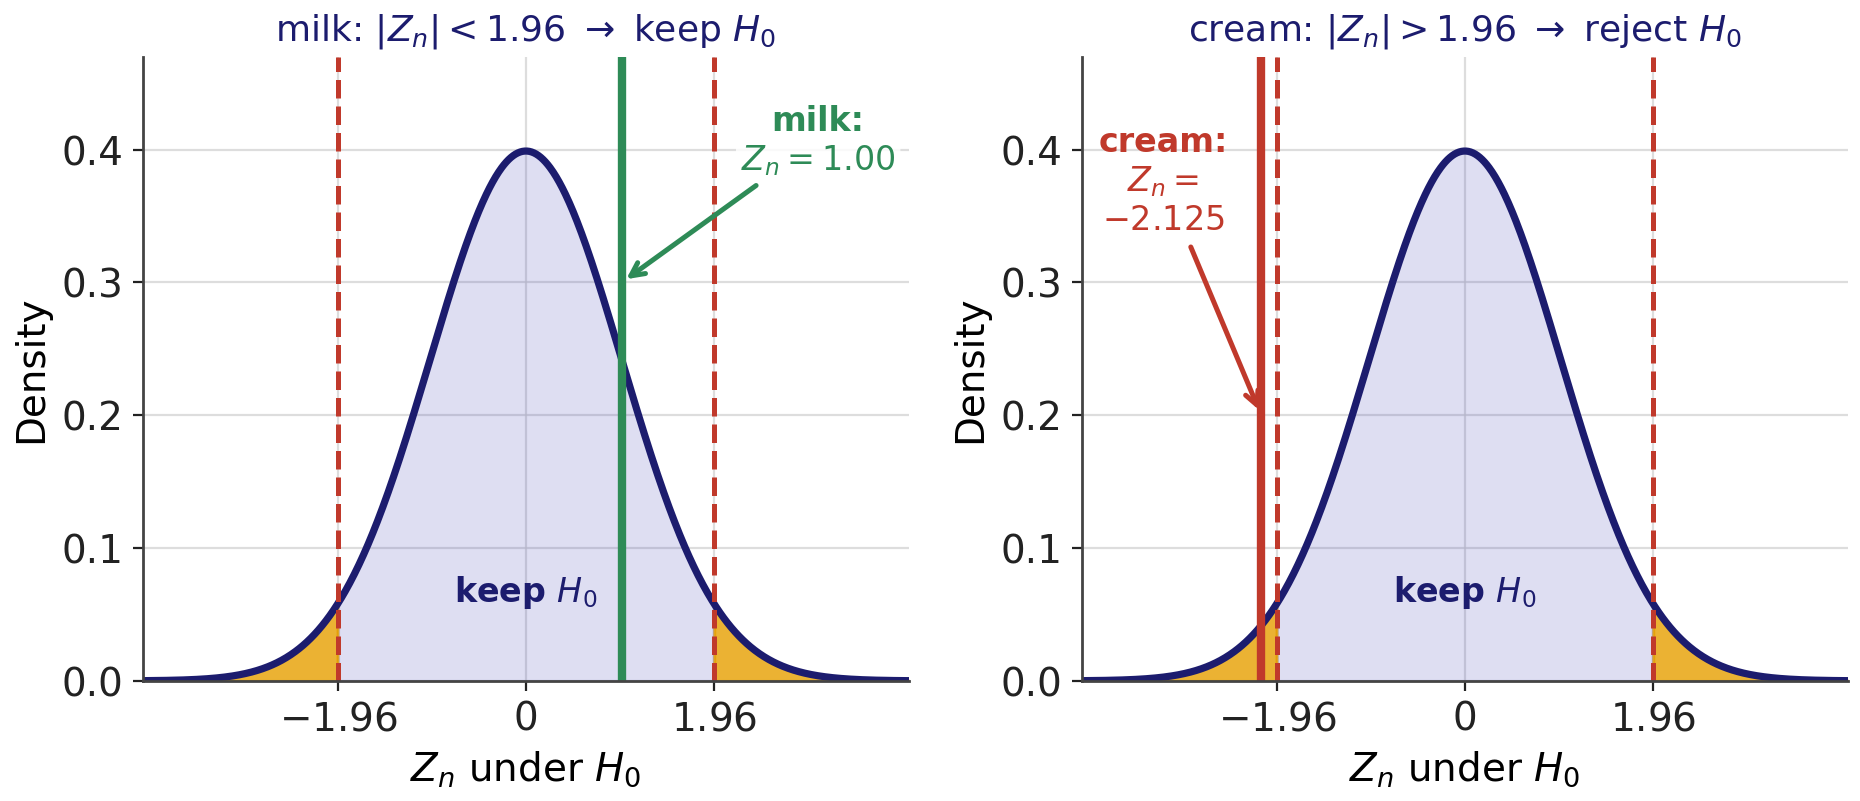
\includegraphics[width=0.97\textwidth,height=0.66\textheight,keepaspectratio]{images/test_milk_cream.png}
  \end{center}
  \footnotesize Two-sided test, known $\sigma$, $\alpha=0.05$: the milk
  statistic ($Z_n=1.00$) stays \emph{inside} the bars $\pm1.96$, the cream
  statistic ($Z_n=-2.125$) lands \emph{beyond} them. The decision is nothing
  more than: \textbf{where does my statistic fall?}
\end{frame}
\note{Talk track: this is the recap picture for the whole section -- one curve
(the $H_0$ world), two bars (the critical values), and the only question:
inside or outside? Milk inside, cream outside. If students can redraw this
from memory, they have understood the classical test.}

\begin{frame}{Exercise -- reaction time (large sample)}
  \begin{block}{Problem statement}
    A training programme is meant to change the baseline reaction time
    $\mu_0 = 250\,$ms. A sample of $n=50$ gives $\bar x = 242$, $s = 30$. Test
    \emph{two-sided} at $\alpha=0.05$.
  \end{block}
  \textbf{Hint:} $t_{0.975;\,49} = 2.0096$ (already close to $1.96$).
\end{frame}

\begin{frame}{Solution -- reaction time}
  \[
    T_n = \frac{242-250}{30/\sqrt{50}} = \frac{-8}{4.2426} = -1.8856,
    \qquad |T_n| = 1.8856 < 2.0096
  \]
  \begin{exampleblock}{Decision \& outlook}
    Keep $H_0$ (two-sided): $p = 2\,F_{t,49}(-1.8856) = \mathbf{0.0653} >
    0.05$. With $n=50\ge 30$ the CLT justifies the $t$-test.
    \emph{Outlook:} had the question -- \emph{before} collecting the data --
    declared only a \emph{shorter} reaction time relevant, a left-sided test
    would have been appropriate, and it would decide differently here (see the
    one-sided exercises). The direction must never be chosen \emph{afterwards}
    because $\bar x<\mu_0$.
  \end{exampleblock}
\end{frame}

% ---- Exercise: delivery time, complete t-test by hand (SfOe Teil 6) ---------------
\begin{frame}{Exercise -- delivery time (complete $t$-test by hand)}
  \begin{block}{Problem statement}
    A logistics provider contractually guarantees an online shop a
    \textbf{mean delivery time of $\mu_0=48$ hours}. The shop's controller wants
    to check whether the actual mean delivery time \emph{deviates} from this --
    both directions matter (too slow: customer complaints; too fast: the shop
    could book a cheaper, slower tariff). For $n=8$ randomly selected
    shipments she records the delivery time (in h):
    \[
      51,\ 39,\ 49,\ 41,\ 47,\ 43,\ 45,\ 45
    \]
    Delivery times are approximately normal, $\sigma$ unknown, $\alpha=0.05$.
  \end{block}
  \begin{enumerate}\setlength{\itemsep}{1pt}
    \item[a)] Compute $\bar x$ and $s$.
    \item[b)] State $H_0$/$H_1$, compute $T_n$ and decide with the critical
              value.
    \item[c)] Compute the $95\,\%$ CI for $\mu$ and show that it agrees with
              the test decision.
  \end{enumerate}
  \textbf{Hint:} $t_{0.975;\,7}=2.3646$.
\end{frame}

\begin{frame}{Solution (1/4) -- delivery time: key figures}
  \textbf{Rule:} $\bar x=\frac1n\sum x_i$, \quad
  $s^2=\frac{1}{n-1}\sum(x_i-\bar x)^2$.
  \begin{center}
    \renewcommand{\arraystretch}{1.15}
    \begin{tabular}{l*{8}{r}r}
      \toprule
      $x_i$            & 51 & 39   & 49 & 41   & 47 & 43   & 45 & 45 & $\sum=360$\\
      $x_i-\bar x$     & 6  & $-6$ & 4  & $-4$ & 2  & $-2$ & 0  & 0  & $\sum=0$\\
      $(x_i-\bar x)^2$ & 36 & 36   & 16 & 16   & 4  & 4    & 0  & 0  & $\sum=112$\\
      \bottomrule
    \end{tabular}
  \end{center}
  \begin{align*}
    \bar x &= \frac{360}{8}=\mathbf{45\ h}, \qquad
    s^2=\frac{112}{8-1}=\frac{112}{7}=16
    \;\Longrightarrow\; s=\mathbf{4\ h}\\[2pt]
    \text{standard error:}\quad \frac{s}{\sqrt n}&=\frac{4}{\sqrt8}
      =\frac{4}{2.8284}=\mathbf{1.4142\ h}
  \end{align*}
  \inworten{The shipments took $45$\,h on average; single values scatter with
  $4$\,h, the sample mean only with $1.41$\,h.}
\end{frame}

\begin{frame}{Solution (2/4) -- delivery time: test with the critical value}
  \textbf{Hypotheses} (two-sided; the direction follows from the question,
  \emph{not} from the data):
  \[
    H_0:\mu=48 \qquad\text{vs.}\qquad H_1:\mu\neq48
  \]
  \textbf{Rule:} $\sigma$ unknown $\Rightarrow$ $t$-test; reject if
  $|T_n|>t_{1-\alpha/2;\,n-1}=t_{0.975;\,7}=2.3646$.
  \begin{align*}
    T_n &= \frac{\bar x-\mu_0}{s/\sqrt n}=\frac{45-48}{1.4142}
         =\frac{-3}{1.4142}=\mathbf{-2.1213}\\[2pt]
    |T_n| &= 2.1213 \;<\; 2.3646
  \end{align*}
  \begin{exampleblock}{Decision}
    $H_0:\mu=48$ is \textbf{not rejected} (narrowly). The observed deviation of
    $3$\,h amounts to just over $2$ standard errors -- with only $n=8$
    shipments this is still compatible with chance; a breach of contract is
    \emph{not} statistically established.
  \end{exampleblock}
\end{frame}

\begin{frame}{Solution (3/4) -- delivery time: CI and duality}
  \textbf{Rule:} $\text{CI}_{0.95}=\bigl[\bar x\pm t_{0.975;\,7}\,s/\sqrt n\bigr]$.
  \begin{align*}
    e &= 2.3646\cdot1.4142=3.344\\
    \text{CI}_{0.95} &= [\,45\pm3.344\,]=\mathbf{[\,41.66\,;\,48.34\,]}\ \text{h}
  \end{align*}
  \begin{block}{Duality CI $\leftrightarrow$ test}
    $\mu_0=48\in[\,41.66\,;\,48.34\,]$ $\Leftrightarrow$
    $|T_n|\le t_{0.975;\,7}$ $\Leftrightarrow$ keep $H_0$ -- the same algebra,
    two readings. That $48$ lies \emph{just} inside the upper bound mirrors the
    narrow $|T_n|=2.12$ vs.\ $2.36$.
  \end{block}
  \inworten{Mean delivery times between $41.7$\,h and $48.3$\,h are compatible
  with the data -- the contractual $48$\,h are (just) among them.}
\end{frame}

\begin{frame}[fragile]{Solution (4/4) -- delivery time: with Python}
\begin{lstlisting}
import numpy as np
from scipy import stats
delivery = np.array([51, 39, 49, 41, 47, 43, 45, 45])    # hours
print(delivery.mean(), delivery.std(ddof=1), round(stats.t.ppf(0.975, df=7), 4))
res = stats.ttest_1samp(delivery, popmean=48)            # two-sided
ci = res.confidence_interval(confidence_level=0.95)
print(f"t = {res.statistic:.4f}, df = {res.df}, p = {res.pvalue:.4f}")
print(f"95% CI: [{ci.low:.2f}, {ci.high:.2f}]")
\end{lstlisting}
  \begin{columns}[T]
    \begin{column}{0.48\textwidth}
      \begin{block}{Output ($\bar x$, $s$, critical value; test; CI)}
\begin{lstlisting}[style=Pyout]
45.0 4.0 2.3646
t = -2.1213, df = 7, p = 0.0716
95% CI: [41.66, 48.34]
\end{lstlisting}
      \end{block}
    \end{column}
    \begin{column}{0.48\textwidth}
      \footnotesize $t$, df and CI agree with the hand calculation. The
      reported $p=0.0716>0.05$ leads to the same decision -- what it means
      exactly is the topic of the next section.
    \end{column}
  \end{columns}
  \trynotebook{section 3.6 ``Exercises''}
\end{frame}
\note{Talk track: this is the complete exam workflow on raw data -- table of
deviations, $s$ with $n-1$, standard error, statistic, critical value, CI,
duality. Let students do a)--c) by hand first, then show that one scipy call
reproduces everything. Point at the $p$-value in the output: it is the bridge
to the next section, where the same exercise returns with the $t$-table.}

% ---- Bridge to the p-value --------------------------------------------------
\begin{frame}{Recap -- and one limitation of the recipe}
  \begin{block}{The recipe in one line}
    Standardise the deviation, compare with the critical value, decide.
  \end{block}
  \begin{center}
    \renewcommand{\arraystretch}{1.4}
    \begin{tabular}{@{}lcccl@{}}
      \toprule
      \textbf{Example} & \textbf{Statistic} & \textbf{Bar} &
        \textbf{Decision} & \textbf{How close?}\\
      \midrule
      milk, $\sigma$ known    & $|Z_n|=1.000$ & $1.960$
        & keep $H_0$            & clear call\\
      cream, $\sigma$ known   & $|Z_n|=2.125$ & $1.960$
        & \textcolor{hsbirot}{reject $H_0$} & close call\\
      cream, $\sigma$ unknown & $|T_n|=2.109$ & $2.131$
        & keep $H_0$            & razor-thin\\
      \bottomrule
    \end{tabular}
  \end{center}
  \begin{block}{Next section}
    All three verdicts are a bare \emph{yes/no} -- the last column is
    invisible in them. The \textbf{$p$-value} puts exactly this -- the
    \emph{strength} of the evidence -- on a continuous $0$--$1$ scale.
  \end{block}
\end{frame}
\note{Talk track: read the table row by row -- same recipe, three very
different situations. Then point at the decision column: it cannot
distinguish the comfortable milk ``keep'' from the razor-thin cream ``keep'',
nor say how decisive the cream rejection was. That missing ``how close?''
column is precisely what the $p$-value will deliver: milk $0.32$, cream
$0.034$ ($\sigma$ known) and $0.052$ ($\sigma$ unknown). Keep it short -- a springboard, not new content.}
% ============================================================================
% SECTION 4: p-VALUE
% ============================================================================
\section[\texorpdfstring{$p$}{p}-value]{The \texorpdfstring{$p$}{p}-Value}

\subsection{Concept}

% ---- Intuition -------------------------------------------------------------
\begin{frame}{The $p$-value -- intuition}
  \begin{block}{A single question}
    ``How \textbf{surprising} are my data if $H_0$ were true?''
  \end{block}
  \begin{itemize}\setlength{\itemsep}{3pt}
    \item \textbf{Small $p$-value} ($\approx 0$): such an extreme result would
          be very rare under $H_0$ $\Rightarrow$ doubt about $H_0$.
    \item \textbf{Large $p$-value} ($\approx 1$): the data are unsurprising
          under $H_0$ $\Rightarrow$ no reason to doubt it (but \emph{not}
          positive proof of $H_0$).
  \end{itemize}
  \kernaussage{The $p$-value measures \emph{how surprising} the data are if
  $H_0$ holds -- the smaller, the stronger the evidence \textbf{against} $H_0$.}
\end{frame}

% ---- Graphical -------------------------------------------------------------
\begin{frame}{The $p$-value -- graphically}
  \begin{center}
    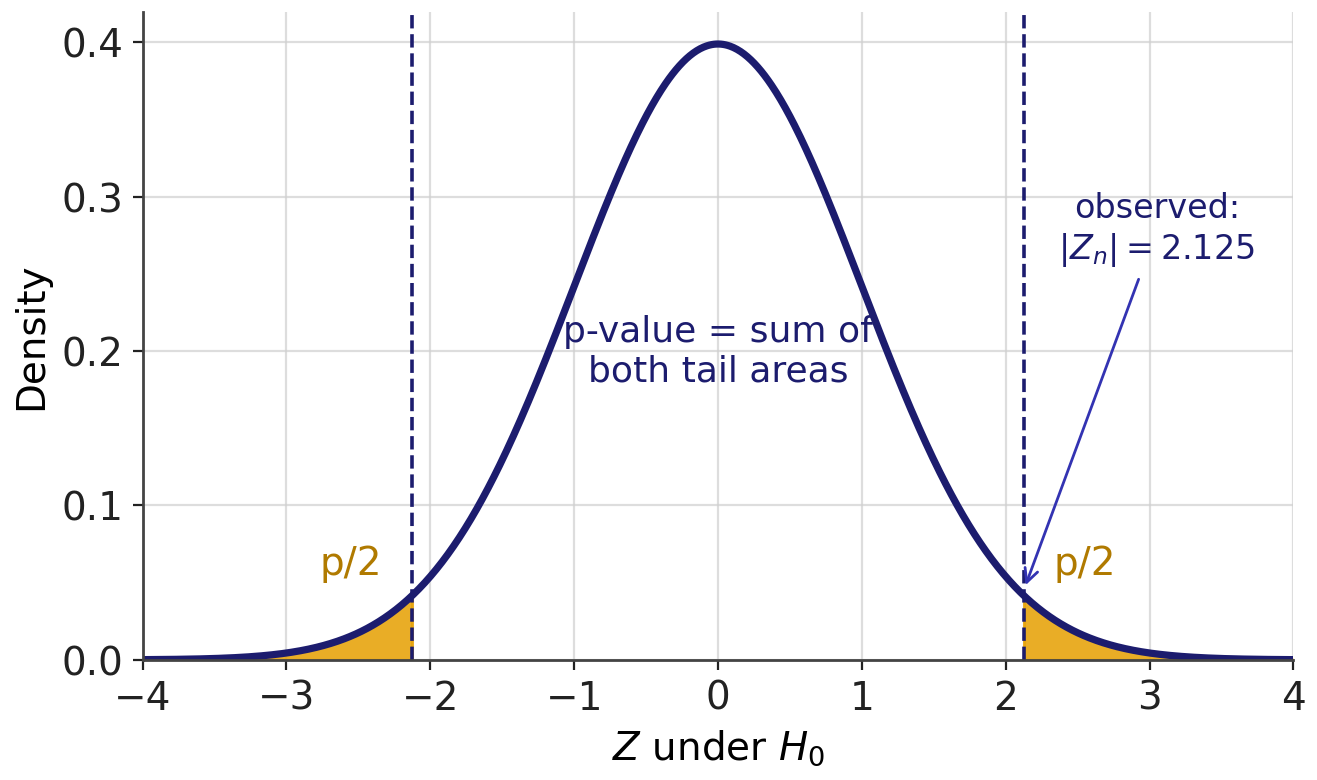
\includegraphics[width=0.80\textwidth,height=0.62\textheight,keepaspectratio]{images/p_value_twosided.png}
  \end{center}
  \footnotesize The (two-sided) $p$-value is the \textbf{total area} in both
  tails that is \emph{at least as extreme} as the observed value.
\end{frame}

% ---- Formal definition -----------------------------------------------------
\begin{frame}{The $p$-value -- definition}
  \begin{block}{Definition}
    The $p$-value is the probability, under the validity of $H_0$, of observing
    a test statistic that is \textbf{at least as extreme} as the one actually
    observed.
  \end{block}
  \begin{itemize}
    \item \textbf{``At least as extreme'' is set by $H_1$:} two-sided
          ($\mu\neq\mu_0$) $=$ both tails $|Z|\ge|Z_n|$; one-sided $=$ only the
          tail in the $H_1$ direction. Same statistic, different $p$.
    \item $0 \le p \le 1$; software (e.g.\ \texttt{scipy.stats}) always reports it.
    \item \textbf{Advantage:} more informative than a bare yes/no -- it
          quantifies the \emph{strength} of the evidence.
  \end{itemize}
\end{frame}
\note{Talk track: read the definition twice, slowly -- every word carries
weight. ``Under the validity of $H_0$'' = we compute in the $H_0$ world.
``At least as extreme'' = the observed value or anything further out, where
``out'' is defined by $H_1$. Warn explicitly: the $p$-value is NOT the
probability that $H_0$ is true -- that misreading is the single most common
exam error (dedicated slide follows).}

% ---- Decision rule + comparison --------------------------------------------
\begin{frame}{Decision rule}
  \begin{alertblock}{One rule for all tests}
    \[
      p < \alpha \;\Longrightarrow\; \text{reject } H_0
      \qquad\qquad
      p \ge \alpha \;\Longrightarrow\; \text{keep } H_0
    \]
  \end{alertblock}
  \begin{columns}[T]
    \begin{column}{0.62\textwidth}
      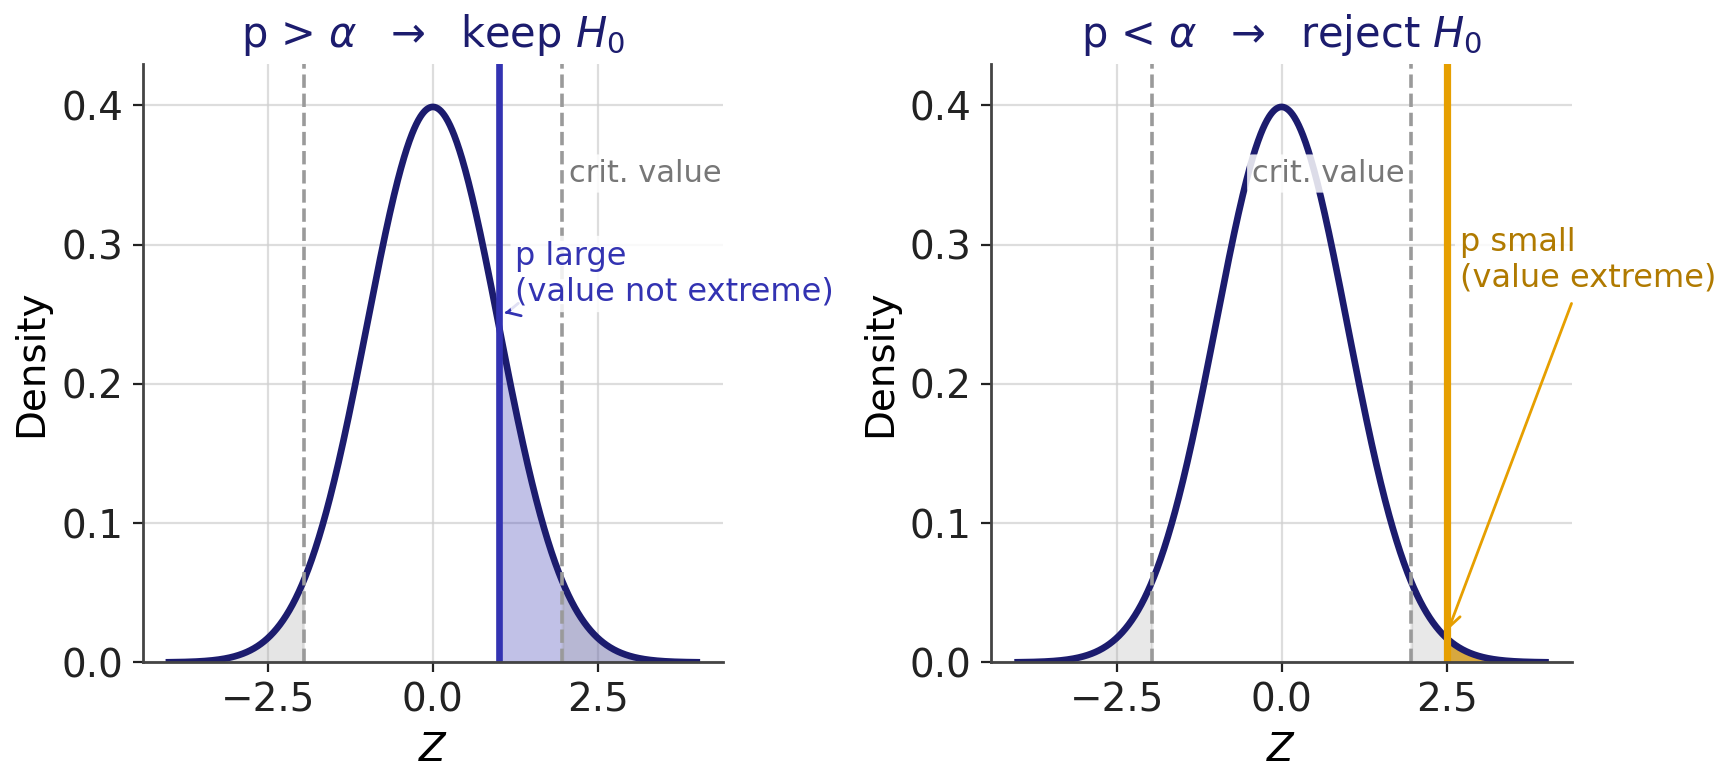
\includegraphics[width=\textwidth,height=0.52\textheight,keepaspectratio]{images/p_value_comparison.png}
    \end{column}
    \begin{column}{0.36\textwidth}
      \footnotesize
      \begin{itemize}\setlength{\itemsep}{4pt}
        \item Left: $p$ large, value in the acceptance region.
        \item Right: $p$ small, value in the rejection region.
        \item $\alpha$ is the ``benchmark''.
      \end{itemize}
    \end{column}
  \end{columns}
\end{frame}

\begin{frame}{Two rules, one decision: critical value $\leftrightarrow$ $p$-value}
  \begin{columns}[T]
    \begin{column}{0.6\textwidth}
      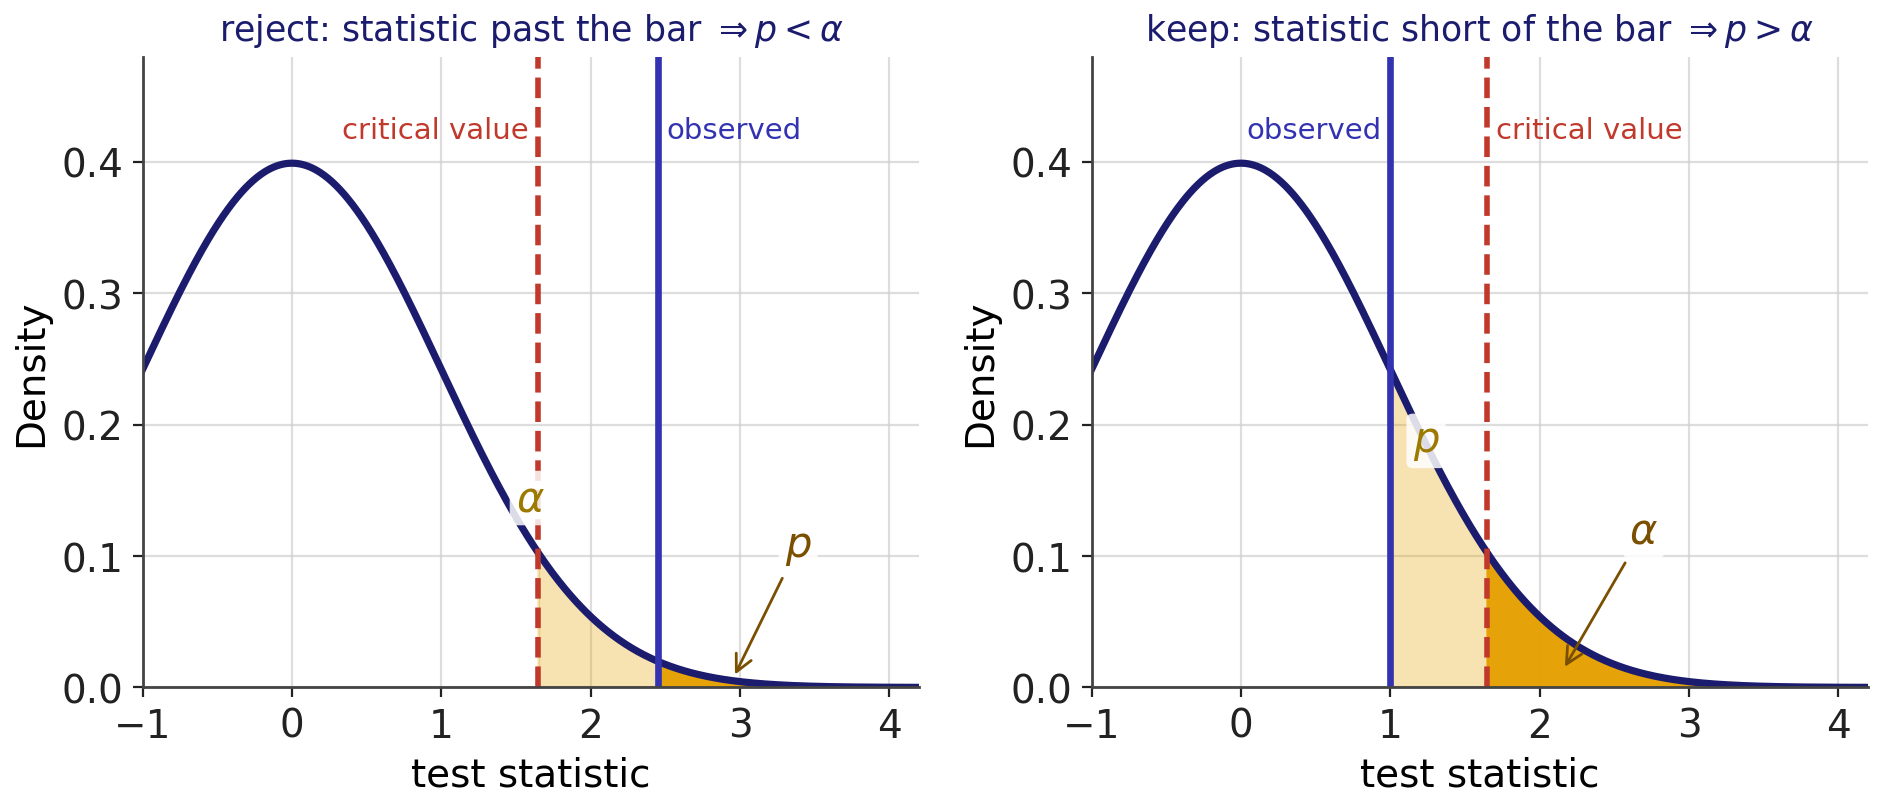
\includegraphics[width=\textwidth,height=0.52\textheight,keepaspectratio]{images/cv_pvalue_link.png}
    \end{column}
    \begin{column}{0.38\textwidth}
      \footnotesize
      \begin{itemize}\setlength{\itemsep}{5pt}
        \item $\alpha$ = tail area beyond the \textbf{critical value} (fixed in
              advance).
        \item $p$ = tail area beyond your \textbf{observed} statistic.
        \item Statistic past the bar $\Leftrightarrow$ its tail is smaller
              $\Leftrightarrow p<\alpha$.
        \item Picture: \emph{right-sided} test ($z_{0.95}=1.645$); two-sided:
              both tails, $z_{0.975}=1.96$.
      \end{itemize}
    \end{column}
  \end{columns}
  \kernaussage{The two decision rules are \textbf{identical}: ``test statistic
  beyond the critical value'' and ``$p<\alpha$'' always agree -- the critical
  value is simply the statistic whose tail area equals $\alpha$.}
\end{frame}

\begin{frame}{Both rules, one verdict -- worked example}
  \textbf{Cream, two-sided, known $\sigma$:} \ $Z_n=-2.125$, \ $\alpha=0.05$.
  \begin{columns}[T]
    \begin{column}{0.48\textwidth}
      \begin{block}{Critical-value rule}
        \[ |Z_n| = 2.125 \;>\; 1.96 = z_{0.975} \]
        \centering $\Rightarrow$ \textbf{reject} $H_0$.
      \end{block}
    \end{column}
    \begin{column}{0.48\textwidth}
      \begin{block}{$p$-value rule}
        \[ p = 2\,\Phi(-2.125) = 0.034 \]
        \centering $0.034 < 0.05 \Rightarrow$ \textbf{reject} $H_0$.
      \end{block}
    \end{column}
  \end{columns}
  \kernaussage{Same data, same $\alpha$, \textbf{same decision} -- because
  $|Z_n|>z_{0.975}$ and $p<\alpha$ are just two ways of saying the observed
  value sits past the bar.}
\end{frame}

\begin{frame}{Exercise -- $p$-value and the choice of $\alpha$}
  \begin{block}{Problem statement}
    A two-sided test with known variance yields $Z_n = 1.85$. Compute the
    $p$-value and decide at $\alpha = 0.05$ and at $\alpha = 0.10$. Check both
    decisions with the critical-value rule.
  \end{block}
  \textbf{Hint:} $\Phi(1.85) = 0.9678$ (table: row $1.8$, column $.05$);
  two-sided as in the worked example: $p=2\,\Phi(-|Z_n|)$; \
  $z_{0.975}=1.96$, \ $z_{0.95}=1.645$.
\end{frame}

\begin{frame}{Solution -- $p$-value and $\alpha$}
  \textbf{Rule:} two-sided $p=2\,\Phi(-|Z_n|)=2\,\bigl(1-\Phi(|Z_n|)\bigr)$
  (symmetry); reject $H_0$ if $p<\alpha$.
  \[
    p = 2\,\bigl(1-\Phi(1.85)\bigr) = 2\cdot 0.0322 = \mathbf{0.0644}
    \qquad(\text{exact, unrounded }\Phi\text{: }0.0643)
  \]
  \begin{itemize}
    \item At $\alpha = 0.05$: \ $0.0644 > 0.05 \Rightarrow$ \textbf{keep} $H_0$.
          \ Check: $|Z_n|=1.85<1.96=z_{0.975}$.
    \item At $\alpha = 0.10$: \ $0.0644 < 0.10 \Rightarrow$ \textbf{reject} $H_0$.
          \ Check: $|Z_n|=1.85>1.645=z_{0.95}$ (two-sided at $10\,\%$ uses
          $z_{1-0.10/2}=z_{0.95}$).
  \end{itemize}
  \kernaussage{The same data can be ``significant'' or not -- $\alpha$ must be
  fixed \emph{in advance}, never chosen to fit the result.}
\end{frame}

\subsection{Calculation}

\begin{frame}{Computing the $p$-value (two-sided)}
  \begin{block}{Known variance}
    \[
      p = 2\cdot\Phi\!\bigl(-|Z_n|\bigr) = P\!\bigl(|Z| > |Z_n|\bigr),
      \quad Z\sim N(0,1)
    \]
  \end{block}
  \begin{block}{Unknown variance}
    \[
      p = 2\cdot F_{t,n-1}\!\bigl(-|T_n|\bigr)
    \]
  \end{block}
  \inworten{\textbf{Why double?} With $H_1:\mu\neq\mu_0$ a deviation in
  \emph{either} direction counts, so ``at least as extreme'' means \emph{both}
  tails $|Z|>|Z_n|$; by symmetry each has area $\Phi(-|Z_n|)$ -- hence the
  factor $2$. (One-sided: a single tail, no doubling.)}
\end{frame}

\begin{frame}{$p$-value -- milk (two variants)}
  \begin{columns}[T]
    \begin{column}{0.48\textwidth}
      \begin{block}{Known variance, $Z_n=1.000$}
        \begin{align*}
          p &= 2\cdot\Phi(-1.00)\\
            &= 2\cdot 0.15866 = 0.3173
        \end{align*}
      \end{block}
    \end{column}
    \begin{column}{0.48\textwidth}
      \begin{block}{Unknown variance, $T_n=0.7947$}
        \begin{align*}
          p &= 2\cdot F_{t,8}(-0.7947)\\
            &= 2\cdot 0.22485 = 0.4497
        \end{align*}
      \end{block}
    \end{column}
  \end{columns}
  \begin{exampleblock}{Decision}
    Both $p$-values $> 0.05 \Rightarrow H_0:\mu=1000$ not rejected.
    The value $0.4497$ matches the \texttt{ttest\_1samp} output.
  \end{exampleblock}
  \footnotesize\textbf{Exact vs.\ table:} the values above use the unrounded
  $\Phi$ and $F_{t,8}$ (software). From the printed $\Phi$ table,
  $\Phi(1.00)=0.8413$ gives $p=2\cdot0.1587=0.3174$. The $t$-table can only
  bracket: $0.7947<1.397=t_{0.90;\,8}$ $\Rightarrow$ $p>2\cdot0.10=0.20$.
\end{frame}

\begin{frame}{$p$-value -- cream (two variants)}
  \begin{columns}[T]
    \begin{column}{0.48\textwidth}
      \begin{block}{Known variance, $Z_n=-2.125$}
        \begin{align*}
          p &= 2\cdot\Phi(-2.125)\\
            &= 2\cdot 0.0168 = \mathbf{0.0336}
        \end{align*}
        $0.0336 < 0.05 \Rightarrow$ reject.
      \end{block}
    \end{column}
    \begin{column}{0.48\textwidth}
      \begin{block}{Unknown variance, $T_n=-2.1086$}
        \begin{align*}
          p &= 2\cdot F_{t,15}(-2.1086)\\
            &= 2\cdot 0.0261 = \mathbf{0.0522}
        \end{align*}
        $0.0522 > 0.05 \Rightarrow$ keep.
      \end{block}
    \end{column}
  \end{columns}
  \kernaussage{The same data set can be just \emph{significant} or just
  \emph{not significant} depending on the assumption about $\sigma$.}
  \footnotesize\textbf{Exact vs.\ table:} exact values (software). With the
  printed tables: $\Phi(2.12)=0.9830$, $\Phi(2.13)=0.9834$ $\Rightarrow$
  $0.0332<p<0.0340$; \ $t$-table, df $=15$: $1.753<2.1086<2.131$
  $\Rightarrow$ $0.05<p<0.10$. Both brackets give the same decisions.
\end{frame}

% ---- p-values with Python ---------------------------------------------------------
\begin{frame}[fragile]{$p$-values with Python}
\begin{lstlisting}
import numpy as np
from scipy import stats
milk = np.array([1005, 1001, 997, 1000, 1001, 998, 999, 999, 1009])
cream = np.array([251, 248, 248, 249, 250, 251, 247, 246,
                  252, 251, 248, 247, 246, 249, 248, 252])
for x, mu0, sigma in [(milk, 1000, 3), (cream, 250, 2)]:
    n = len(x)
    z = (x.mean() - mu0) / (sigma / np.sqrt(n))           # sigma known
    t = (x.mean() - mu0) / (x.std(ddof=1) / np.sqrt(n))   # sigma estimated
    p_z = 2 * stats.norm.sf(abs(z))                       # 2 * (1 - Phi(|z|))
    p_t = 2 * stats.t.sf(abs(t), df=n - 1)                # 2 * (1 - F_t,n-1(|t|))
    print(f"z = {z:.4f}, p = {p_z:.4f} | t = {t:.4f}, p = {p_t:.4f}")
\end{lstlisting}
  \begin{columns}[T]
    \begin{column}{0.56\textwidth}
      \textbf{Output} (milk, cream):
\begin{lstlisting}[style=Pyout]
z = 1.0000, p = 0.3173 | t = 0.7947, p = 0.4497
z = -2.1250, p = 0.0336 | t = -2.1086, p = 0.0522
\end{lstlisting}
    \end{column}
    \begin{column}{0.40\textwidth}
      \footnotesize \texttt{sf} $=1-F$ (survival function). The $t$-row
      equals \texttt{ttest\_1samp(x, mu0)}.
    \end{column}
  \end{columns}
  \trynotebook{section 4.2 ``Calculation''}
\end{frame}

\begin{frame}{$p$-value -- typical misconceptions}
  \begin{alertblock}{What the $p$-value is \emph{not}}
    \begin{itemize}
      \item \textbf{Not} the probability that $H_0$ is true.
      \item A large $p$-value does \textbf{not prove} $H_0$ -- it only shows
            \emph{no contradiction}.
    \end{itemize}
  \end{alertblock}
  \begin{block}{Correct -- mind the direction}
    The $p$-value is the probability \emph{of the data (or more extreme)}
    \textbf{assuming} $H_0$ (chance) holds: $P(\text{data}\mid H_0)$. It
    \emph{conditions on} chance; it does \textbf{not} give the probability that
    chance was the \emph{cause}, $P(H_0\mid\text{data})$.
  \end{block}
\end{frame}
\note{Talk track: use the courtroom again -- $P(\text{evidence}\mid\text{innocent})$
is not $P(\text{innocent}\mid\text{evidence})$. Concrete anchor: ``the
probability that a randomly tested person has these symptoms IF healthy'' vs.\
``the probability the person is healthy GIVEN the symptoms'' -- clearly
different. Also stress the second bullet: a large $p$ means the data cannot
distinguish $H_0$ from nearby alternatives -- absence of evidence, not
evidence of absence.}

\begin{frame}{Significant $\neq$ important -- the large-$n$ trap}
  \begin{block}{The $p$-value measures evidence, not size}
    With enough data, \emph{any} tiny deviation from $\mu_0$ becomes
    statistically significant -- even one that is practically irrelevant.
  \end{block}
  \begin{exampleblock}{Milk machine, observed $\bar x = 1000.2$ ml ($\mu_0=1000$, $\sigma=3$)}
    \centering
    \renewcommand{\arraystretch}{1.15}
    \begin{tabular}{lccl}
      \toprule
      & $Z_n$ & $p$ (two-sided) & verdict at $\alpha=0.05$\\
      \midrule
      $n=9$       & $0.20$ & $0.84$      & not significant\\
      $n=10\,000$ & $6.67$ & $<0.0001$   & \textbf{highly} significant\\
      \bottomrule
    \end{tabular}
  \end{exampleblock}
  \kernaussage{The same irrelevant $0.2$\,ml deviation -- invisible at $n=9$,
  ``highly significant'' at $n=10\,000$. So report the \textbf{effect size and
  the CI}, not just $p$.}
\end{frame}
\note{Talk track: significance answers ``is there evidence of ANY deviation?'',
not ``is the deviation large enough to matter?''. With $n=10\,000$ the SE is
$0.03$\,ml -- the test becomes a microscope. Flip side (links to power): with
small $n$, even an important deviation often stays invisible. Practical rule
for the students: $p$-value for evidence, CI for magnitude -- always read both.}
\subsection{Exercises}

\begin{frame}{Exercise -- interpret the $p$-value (concept)}
  \begin{block}{Which statements are correct? \ ($p = 0.03$, $\alpha=0.05$)}
    \begin{enumerate}
      \item ``There is a $3\,\%$ probability that $H_0$ is true.''
      \item ``If $H_0$ were true, data this extreme occur in $3\,\%$ of samples.''
      \item ``We reject $H_0$ at $\alpha=0.05$.''
      \item ``The effect is large and important.''
    \end{enumerate}
  \end{block}
\end{frame}

\begin{frame}{Solution -- interpret the $p$-value}
  \begin{exampleblock}{Answers}
    \begin{enumerate}
      \item \textbf{Wrong}: $p$ is $P(\text{data}\mid H_0)$, not
            $P(H_0\mid \text{data})$.
      \item \textbf{Correct}: that is exactly the definition.
      \item \textbf{Correct}: $0.03 < 0.05$.
      \item \textbf{Wrong}: significance $\neq$ effect size; a tiny effect can
            be significant with large $n$.
    \end{enumerate}
  \end{exampleblock}
  \kernaussage{A small $p$-value signals \emph{evidence against $H_0$} -- not
  the probability of $H_0$, and not the size or importance of the effect.}
\end{frame}

% ---- Exercise: bracketing the p-value with the t-table (SfOe Teil 6) ---------------
\begin{frame}{Exercise -- bracketing the $p$-value with the $t$-table}
  \begin{block}{Problem statement}
    Delivery-time exercise (section ``Hypothesis tests''): two-sided $t$-test
    with $T_n=-2.1213$ and df $=7$. In the exam there is no software -- only
    the row df $=7$ of the $t$-table:
    \begin{center}
      \renewcommand{\arraystretch}{1.2}
      \begin{tabular}{l|ccccc}
        \toprule
        upper-tail probability $P(T>t)$ & $0.10$ & $0.05$ & $0.025$ & $0.01$ & $0.005$\\
        \midrule
        $t$ (df $=7$) & $1.415$ & $1.895$ & $2.365$ & $2.998$ & $3.499$\\
        \bottomrule
      \end{tabular}
    \end{center}
  \end{block}
  \begin{enumerate}\setlength{\itemsep}{1pt}
    \item[a)] Bracket the two-sided $p$-value from below and above.
    \item[b)] Decide at $\alpha=0.05$ and at $\alpha=0.10$.
    \item[c)] Which Python command gives the exact value?
  \end{enumerate}
\end{frame}

\begin{frame}[fragile]{Solution -- bracketing the $p$-value with the $t$-table}
  \small
  \textbf{Rule:} two-sided $p=2\cdot P(T>|T_n|)$; the table gives $P(T>t)$
  only at a few points -- so \emph{bracket}.
  \[
    \text{\textbf{a)}}\quad 1.895<|T_n|=2.121<2.365
      \;\Longrightarrow\; 0.025<P(T>2.121)<0.05
      \;\Longrightarrow\; \mathbf{0.05<p<0.10}
  \]
  \textbf{b)} $\alpha=0.05$: $p>0.05\Rightarrow$ \textbf{keep} $H_0$ (as
  $|T_n|<2.365$). \quad $\alpha=0.10$: $p<0.10\Rightarrow$ \textbf{reject}
  $H_0$ (as $|T_n|>1.895$).
  \begin{block}{c) exactly, with Python}
\begin{lstlisting}
from scipy import stats
print(round(2 * stats.t.cdf(-2.1213, df=7), 4))        # exact two-sided p-value: 0.0716
\end{lstlisting}
  \end{block}
  \kernaussage{The table yields only an \emph{interval} for $p$ -- enough for
  the decision ``$p<\alpha$?''; critical value and $p$-value always agree.}
  \trynotebook{section 4.3 ``Exercises''}
\end{frame}
\note{Talk track: exam-relevant skill. Draw the df $=7$ row as a ruler, mark
$2.121$ between $1.895$ and $2.365$, read the tail areas $0.05$ and $0.025$
above them -- then DOUBLE for two-sided. Most common error: forgetting the
factor $2$ (giving $0.025<p<0.05$ and the wrong decision at $\alpha=0.05$).}

% ---- Exam-style exercise: coffee roastery (mock exam 5, task 3) -------------------
\begin{frame}{Exercise -- coffee roastery (exam-style, from A to Z)}
  \begin{block}{Problem statement}
    A coffee roastery fills tins with a target net weight of
    $\mu_0=1000$\,g. From long-term process monitoring the standard deviation
    is \emph{known}: $\sigma=40$\,g. After a refit, a sample of $n=64$ tins
    gives $\bar x=1012$\,g. Test two-sided at $\alpha=0.05$.
  \end{block}
  \begin{enumerate}\setlength{\itemsep}{1pt}
    \item[a)] State the hypotheses.
    \item[b)] Compute the standard error $\sigma/\sqrt n$ and the test
              statistic $Z_n$.
    \item[c)] Give the critical value and make the test decision.
    \item[d)] Compute the $p$-value with the $\Phi$-table. Which Python command
              gives it?
    \item[e)] Compute the $95\,\%$ CI for $\mu$. What does it imply for
              $H_0:\mu=1000$?
    \item[f)] A second check sample gives $n=25$, $\bar x=1012$\,g and an
              \emph{estimated} $s=40$\,g. Compute the $95\,\%$ CI
              ($t_{0.975;\,24}=2.0639$). Would $H_0$ be rejected now?
  \end{enumerate}
\end{frame}
\note{Talk track: an exam task in miniature -- let students work in pairs
for 10 minutes with the $\Phi$-table only. The final part f) is the
comparison that matters: same $\bar x$, but estimated $\sigma$ and smaller
$n$ flip the decision.}

\begin{frame}{Solution (1/3) -- coffee roastery: test with the critical value}
  \textbf{a)} Deviations in \emph{both} directions matter (too little:
  consumer protection; too much: cost):
  \[
    H_0:\mu=1000 \qquad\text{vs.}\qquad H_1:\mu\neq1000
  \]
  \textbf{b)} $\sigma$ known $\Rightarrow$ $z$-test (Gauss test):
  \[
    \mathrm{SE}=\frac{\sigma}{\sqrt n}=\frac{40}{\sqrt{64}}=\frac{40}{8}=\mathbf{5\ g},
    \qquad
    Z_n=\frac{\bar x-\mu_0}{\mathrm{SE}}=\frac{1012-1000}{5}=\mathbf{2.40}
  \]
  \textbf{c)} Two-sided: $\alpha/2=0.025$ in each tail, critical value
  $z_{0.975}=1.96$ (table: $\Phi(1.96)=0.9750$).
  \begin{alertblock}{Decision}
    $|Z_n|=2.40>1.96$ $\Rightarrow$ $H_0$ is \textbf{rejected}: the mean fill
    weight deviates significantly from $1000$\,g -- upwards. Readjusting the
    machine saves coffee.
  \end{alertblock}
\end{frame}

\begin{frame}[fragile]{Solution (2/3) -- coffee roastery: $p$-value and CI}
  \textbf{d)} Table: $\Phi(2.40)=0.9918$, so
  \[
    p=2\,\bigl(1-\Phi(2.40)\bigr)=2\cdot0.0082=\mathbf{0.0164}<0.05
    \;\Rightarrow\;\text{reject } H_0 .
  \]
  {\small If the machine were set correctly, a deviation at least this large
  would occur in only $1.64\,\%$ of all samples.}
\begin{lstlisting}
from scipy import stats
z = (1012 - 1000) / (40 / 64 ** 0.5)
print(z, round(2 * stats.norm.sf(abs(z)), 4))           # z and two-sided p-value
\end{lstlisting}
  \vspace{-4pt}
\begin{lstlisting}[style=Pyout]
2.4 0.0164
\end{lstlisting}
  \[
    \text{\textbf{e)}}\quad 1012\pm1.96\cdot5=1012\pm9.8\ \Rightarrow\
    \text{CI}_{0.95}=\mathbf{[\,1002.2\,;\,1021.8\,]}\ \text{g}
  \]
  {\small $1000\notin$ CI $\Rightarrow$ $H_0$ is rejected -- consistent with
  $|Z_n|>1.96$ and $p<0.05$ (duality).}
  \trynotebook{section 4.3 ``Exercises''}
\end{frame}

\begin{frame}{Solution (3/3) -- coffee roastery: estimated $\sigma$}
  \textbf{f)} Now $\sigma$ is \emph{estimated} $\Rightarrow$ $t$-quantile with
  df $=24$:
  \[
    \frac{s}{\sqrt n}=\frac{40}{5}=8,\qquad
    1012\pm2.0639\cdot8=1012\pm16.51
    \ \Rightarrow\ \mathbf{[\,995.49\,;\,1028.51\,]}\ \text{g}
  \]
  \begin{center}
    \small\renewcommand{\arraystretch}{1.25}
    \begin{tabular}{lcc}
      \toprule
       & $\sigma=40$ known, $n=64$ & $s=40$ estimated, $n=25$\\
      \midrule
      standard error & $40/8=5$ & $40/5=8$\\
      quantile & $z_{0.975}=1.96$ & $t_{0.975;\,24}=2.0639$\\
      $95\,\%$ CI & $[\,1002.2\,;\,1021.8\,]$ & $[\,995.49\,;\,1028.51\,]$\\
      contains $\mu_0=1000$? & no $\to$ reject & yes $\to$ keep\\
      \bottomrule
    \end{tabular}
  \end{center}
  \kernaussage{The second interval is wider for \textbf{two} reasons: the
  smaller sample \emph{and} the larger $t$-quantile for the estimated spread.
  Now $1000$ lies inside -- $H_0$ would \emph{not} be rejected.}
\end{frame}
\note{Talk track: this is a complete exam task (adapted from the mock exams).
Typical errors to name: $t$ instead of $z$ although $\sigma$ is known;
$1.645$ instead of $1.96$ for a two-sided test; forgetting the factor $2$ in
the $p$-value; forgetting $\sqrt n$ ($Z_n=12/40=0.3$); reading the CI as
``$\mu$ lies inside with $95\,\%$ probability''.}

% ============================================================================
% SECTION 5: ONE-SIDED TESTS
% ============================================================================
\section[One-sided]{One-Sided Tests}

\subsection{Motivation}

\begin{frame}{When only one direction matters}
  \begin{block}{The idea}
    In a two-sided test \emph{any} departure from $\mu_0$ counts against
    $H_0$. Often, though, a deviation is a \textbf{problem in only one
    direction} -- the other direction is harmless or even welcome.
  \end{block}
  \begin{columns}[T]
    \begin{column}{0.48\textwidth}
      \begin{exampleblock}{Too little in the bottle}
        For consumer protection only \emph{underfilling} ($\mu<1000$) is
        critical -- overfilling does not harm the customer.
      \end{exampleblock}
    \end{column}
    \begin{column}{0.48\textwidth}
      \begin{exampleblock}{Unemployment insurance}
        Only if the rate \emph{exceeds} a threshold do contributions fall
        short. A lower rate causes no problem.
      \end{exampleblock}
    \end{column}
  \end{columns}
  \kernaussage{The \emph{question} -- not the data -- decides the direction.
  The deviation we truly care about defines $H_1$, and the \emph{whole}
  $\alpha$ goes on that one side instead of $\alpha/2$ on each.}
\end{frame}

\begin{frame}{Business examples -- one direction only}
  \begin{center}
    \renewcommand{\arraystretch}{1.5}
    \begin{tabular}{@{}p{7.8cm}cc@{}}
      \toprule
      \textbf{You want evidence that \ldots} & \textbf{$H_1$}
        & \textbf{Direction}\\
      \midrule
      the new ad campaign \emph{raises} the conversion rate
        & $\mu > \mu_0$ & right-sided\\
      the new process \emph{lowers} the average unit cost
        & $\mu < \mu_0$ & left-sided\\
      \bottomrule
    \end{tabular}\\[4pt]
    {\footnotesize In both cases $H_0:\mu=\mu_0$, as before.}
  \end{center}
  \kernaussage{As in the two-sided case, the claim goes into $H_1$ -- but now
  its \emph{inequality} also fixes the side on which we reject.}
\end{frame}

\begin{frame}{How to find the critical value -- 3 steps}
  \begin{enumerate}\setlength{\itemsep}{4pt}
    \item \textbf{Direction} (read from $H_1$): one-sided or two-sided?
    \item \textbf{Tail probability:}
      \begin{itemize}\footnotesize
        \item two-sided $\to$ \emph{split} $\alpha$: use the $1-\alpha/2$
              quantile ($\pm$ value),
        \item one-sided $\to$ keep $\alpha$ \emph{whole}: use the $1-\alpha$
              quantile (one value, on the $H_1$ side).
      \end{itemize}
    \item \textbf{Which table?} $\sigma$ known $\to z$ (normal);
          $\sigma$ unknown $\to t$ with $\mathrm{df}=n-1$.
  \end{enumerate}
  \begin{exampleblock}{$\alpha=0.05$ -- the resulting critical values}
    known $\sigma$:\ two-sided $z_{0.975}=1.96$, \ one-sided $z_{0.95}=1.645$
    ($\Phi$ table).\\
    unknown $\sigma$, $n=12$:\ two-sided $t_{0.975;\,11}=2.20$, \ one-sided
    $t_{0.95;\,11}=1.80$ (\texttt{stats.t.ppf}; the $t$-table follows).
  \end{exampleblock}
\end{frame}
\note{Talk track: walk the 3 steps aloud at $\alpha=0.05$. The ONLY one- vs
two-sided difference is whether you split $\alpha$ ($1-\alpha/2$) or not
($1-\alpha$). Then ``known $\sigma\to z$, unknown $\to t$ with $n-1$''. Have
them read both $1.96$ and $1.645$ off the table so they SEE the bar move
inward. Common error: using $1-\alpha$ for a two-sided test (or vice versa).}

\begin{frame}{One-sided critical values -- left and right}
  \begin{center}
    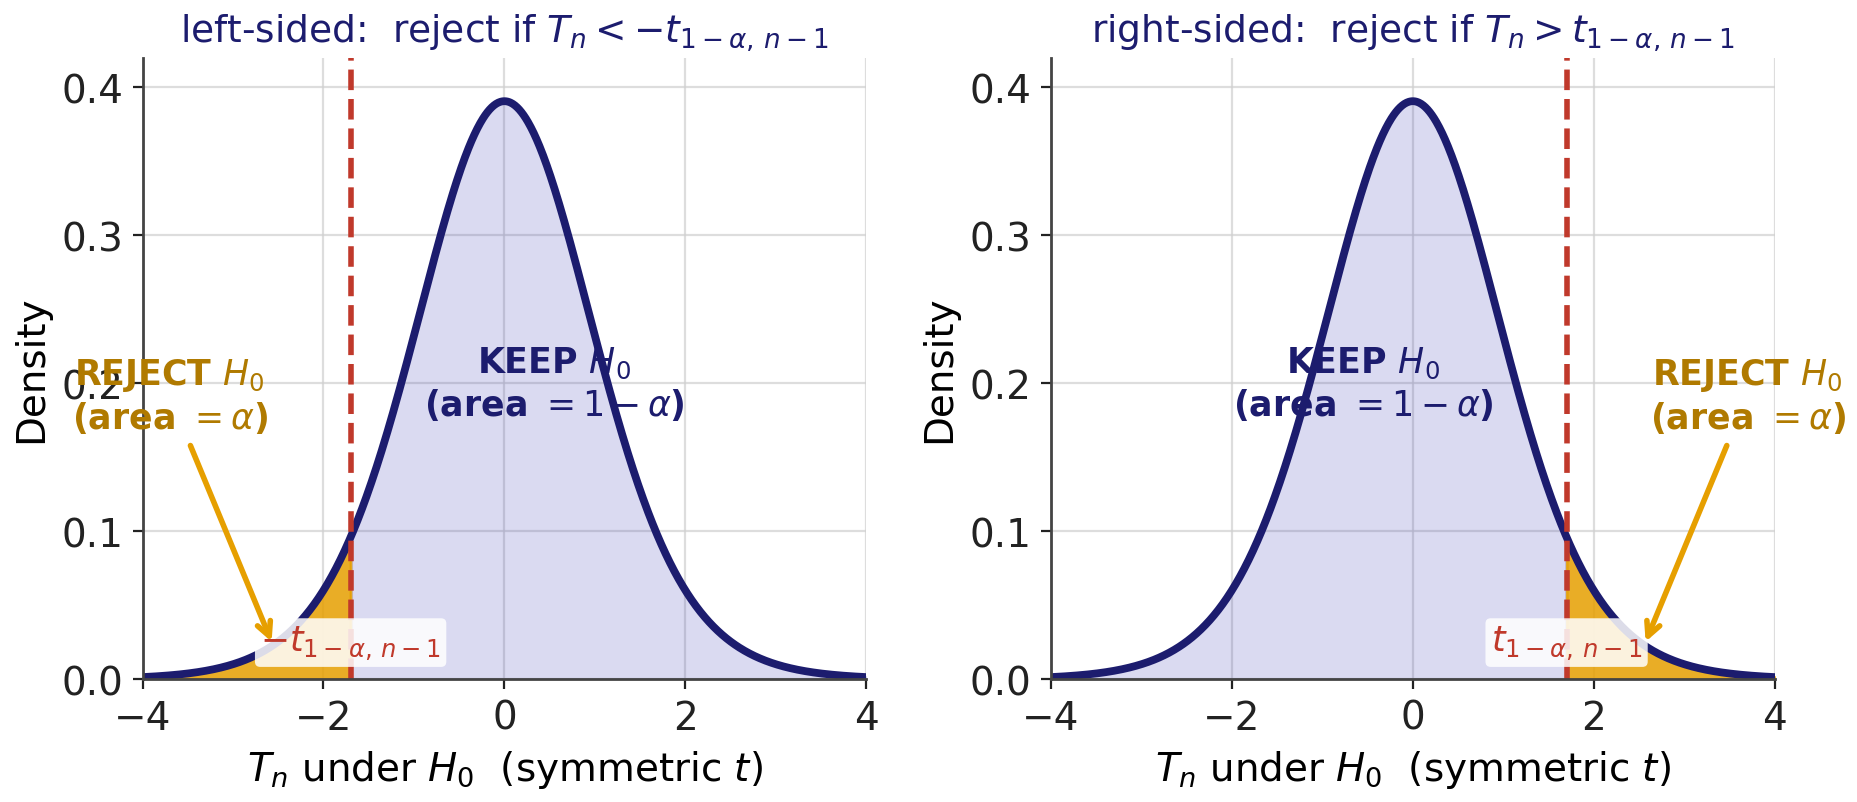
\includegraphics[width=0.96\textwidth,height=0.66\textheight,keepaspectratio]{images/critical_value_onesided.png}
  \end{center}
  \footnotesize The whole rejection area $\alpha$ sits in \emph{one} tail --
  left for ``too small'', right for ``too large''. The curve is the
  \textbf{symmetric} $t$-distribution: only the side changes, the shape never
  does.
\end{frame}
\note{Talk track: point at the picture. ``Same bell curve -- the whole $\alpha$
just moves into one tail.'' Left tail tests ``too small'', right tail ``too
large''. Stress the curve is the symmetric $t$ -- it never becomes skewed. Ask
the room: ``if $T_n$ lands in the blue, what do we do?'' (keep $H_0$). Common
habit to break: shading both tails -- one-sided means ONE tail.}

\begin{frame}{The golden rule of one-sided tests}
  \begin{alertblock}{If you remember only one sentence}
    We reject $H_0$ when the sample result is \textbf{sufficiently extreme in
    the direction specified by the alternative hypothesis} $H_1$.
  \end{alertblock}
  \begin{center}
    \renewcommand{\arraystretch}{1.5}
    \begin{tabular}{@{}l@{\hspace{3mm}}c@{\hspace{3mm}}l@{}}
      \footnotesize $H_1:\mu<\mu_0$ \emph{(smaller)} &
        \begin{tikzpicture}[baseline=-3pt]
          \path (-2.3,0) (2.55,0);   % same width in every row (alignment)
          \draw[->,gray] (-2.2,0)--(2.45,0);
          \draw[line width=4pt,hsbiorange] (-2.2,0)--(-1.45,0);
          \draw (0,0.13)--(0,-0.13) node[below,font=\tiny]{$\mu_0$};
        \end{tikzpicture}
        & \footnotesize reject if $z$ very \textbf{negative}\\
      \footnotesize $H_1:\mu>\mu_0$ \emph{(larger)} &
        \begin{tikzpicture}[baseline=-3pt]
          \path (-2.3,0) (2.55,0);   % same width in every row (alignment)
          \draw[->,gray] (-2.2,0)--(2.45,0);
          \draw[line width=4pt,hsbiorange] (1.45,0)--(2.2,0);
          \draw (0,0.13)--(0,-0.13) node[below,font=\tiny]{$\mu_0$};
        \end{tikzpicture}
        & \footnotesize reject if $z$ very \textbf{positive}\\
      \footnotesize $H_1:\mu\neq\mu_0$ \emph{(different)} &
        \begin{tikzpicture}[baseline=-3pt]
          \path (-2.3,0) (2.55,0);   % same width in every row (alignment)
          \draw[->,gray] (-2.2,0)--(2.45,0);
          \draw[line width=4pt,hsbiorange] (-2.2,0)--(-1.6,0);
          \draw[line width=4pt,hsbiorange] (1.6,0)--(2.2,0);
          \draw (0,0.13)--(0,-0.13) node[below,font=\tiny]{$\mu_0$};
        \end{tikzpicture}
        & \footnotesize reject if $|z|$ very \textbf{large} (either way)\\
    \end{tabular}
  \end{center}
  \kernaussage{The inequality in $H_1$ points straight at the rejection region
  (orange): ``$<$'' $\to$ left tail, ``$>$'' $\to$ right tail, ``$\neq$'' $\to$
  both.}
\end{frame}
\note{Talk track: make them memorise the one sentence in the alert box -- it
decides every one-sided question. Drill with quick calls: ``$H_1:\mu>5$, where
do we reject?'' (right tail) -- ``$z=-3$ in that test?'' (keep! wrong
direction). The orange bars in the table are the visual anchor.}

% ---- Lawyer's argument (evidence scale) ------------------------------------
\begin{frame}{A left-sided test as a lawyer's argument}
  \textbf{Your claim} ($H_1:\mu<10$): ``the true mean is \emph{smaller} than
  $10$.'' \ The sample mean $\bar x$ is your evidence:
  \begin{center}
    \renewcommand{\arraystretch}{1.25}
    \begin{tabular}{ccccc}
      \toprule
      $\bar x=8$ & $\bar x=9$ & $\bar x=10$ & $\bar x=11$ & $\bar x=12$\\
      \midrule
      strong \emph{for} & some \emph{for} & neutral & against & against\\
      \bottomrule
    \end{tabular}
  \end{center}
  \begin{itemize}\setlength{\itemsep}{2pt}
    \item Below $10$ $\Rightarrow$ evidence \emph{for} $H_1$; if extreme enough,
          \textbf{reject} $H_0$.
    \item $\bar x=12$ is far from $10$ but in the \emph{wrong} direction -- it
          gives \textbf{no} support for ``$\mu<10$''.
  \end{itemize}
  \kernaussage{The test asks whether the evidence \emph{in the $H_1$ direction}
  is strong enough to reject $H_0$ -- a big deviation the wrong way counts for
  nothing.}
\end{frame}

\begin{frame}{Critical values of the standard normal $N(0,1)$}
  \begin{center}
    \renewcommand{\arraystretch}{1.35}
    \begin{tabular}{cccc}
      \toprule
      Confidence $1-\alpha$ & $\alpha$ & \textbf{one-sided} $z_{1-\alpha}$
        & \textbf{two-sided} $z_{1-\alpha/2}$\\
      \midrule
      $90\,\%$   & $0.10$  & $1.282$ & $1.645$\\
      $95\,\%$   & $0.05$  & $1.645$ & $1.960$\\
      $98\,\%$   & $0.02$  & $2.054$ & $2.326$\\
      $99\,\%$   & $0.01$  & $2.326$ & $2.576$\\
      $99.9\,\%$ & $0.001$ & $3.090$ & $3.291$\\
      \bottomrule
    \end{tabular}
  \end{center}
  \inworten{Pattern: the two-sided value at level $\alpha$ equals the one-sided
  value at level $\alpha/2$ -- e.g.\ two-sided $95\%=1.96=$ one-sided $97.5\%$.}
\end{frame}

\begin{frame}{Critical values of the $t$-distribution $t_{\mathrm{df}}$}
  \begin{center}
    \scriptsize
    \renewcommand{\arraystretch}{0.95}
    \begin{tabular}{r|ccccc}
      \toprule
      & \multicolumn{5}{c}{\textbf{upper-tail probability}}\\
      & \multicolumn{5}{c}{(one-sided $\alpha$ \ $\mid$\ two-sided $\alpha/2$)}\\
      \cmidrule(l){2-6}
      df $=n-1$ & $0.10$ & $0.05$ & $0.025$ & $0.01$ & $0.005$\\
      \midrule
      $1$   & $3.078$ & $6.314$ & $12.706$ & $31.821$ & $63.657$\\
      $2$   & $1.886$ & $2.920$ & $4.303$  & $6.965$  & $9.925$\\
      $3$   & $1.638$ & $2.353$ & $3.182$  & $4.541$  & $5.841$\\
      $4$   & $1.533$ & $2.132$ & $2.776$  & $3.747$  & $4.604$\\
      $5$   & $1.476$ & $2.015$ & $2.571$  & $3.365$  & $4.032$\\
      $6$   & $1.440$ & $1.943$ & $2.447$  & $3.143$  & $3.707$\\
      $7$   & $1.415$ & $1.895$ & $2.365$  & $2.998$  & $3.499$\\
      $8$   & $1.397$ & $1.860$ & $2.306$  & $2.896$  & $3.355$\\
      $9$   & $1.383$ & $1.833$ & \cellcolor{hsbiorange!35}$2.262$ & $2.821$ & $3.250$\\
      $10$  & $1.372$ & $1.812$ & $2.228$  & $2.764$  & $3.169$\\
      $15$  & $1.341$ & $1.753$ & $2.131$  & $2.602$  & $2.947$\\
      $20$  & $1.325$ & $1.725$ & $2.086$  & $2.528$  & $2.845$\\
      $30$  & $1.310$ & $1.697$ & $2.042$  & $2.457$  & $2.750$\\
      $60$  & $1.296$ & $1.671$ & $2.000$  & $2.390$  & $2.660$\\
      $\infty$ & $1.282$ & $1.645$ & $1.960$ & $2.326$ & $2.576$\\
      \bottomrule
    \end{tabular}
  \end{center}
  \scriptsize Highlighted: $t_{0.975;\,9}=2.262$ (two-sided $95\%$, $n=10$); the $\infty$-row is the normal.
\end{frame}

\begin{frame}{How to read the tables -- worked lookups}
  \begin{block}{Three questions, every time}
    (1) one- or two-sided? \quad (2) which $\alpha$? \quad (3) $z$ or $t$ (df $=n-1$)?
  \end{block}
  \begin{columns}[T]
    \begin{column}{0.48\textwidth}
      \textbf{Normal} ($\sigma$ known):
      \begin{itemize}\footnotesize\setlength{\itemsep}{2pt}
        \item two-sided, $\alpha=0.05$ $\to$ column $1-\tfrac{\alpha}{2}=0.975$
              $\to z=1.96$.
        \item one-sided, $\alpha=0.05$ $\to$ $1-\alpha=0.95$ $\to z=1.645$.
      \end{itemize}
    \end{column}
    \begin{column}{0.48\textwidth}
      {\boldmath\textbf{$t$}} ($\sigma$ unknown), $n=10\Rightarrow$ df$=9$:
      \begin{itemize}\footnotesize\setlength{\itemsep}{2pt}
        \item two-sided, $\alpha=0.05$ $\to$ upper-tail $0.025$ $\to t=2.262$.
        \item one-sided, $\alpha=0.05$ $\to$ upper-tail $0.05$ $\to t=1.833$.
      \end{itemize}
    \end{column}
  \end{columns}
  \kernaussage{Two-sided \emph{halves} the tail probability ($\alpha\to\alpha/2$);
  the $t$-row is $\mathrm{df}=n-1$. As df grows, the $t$-value slides towards $z$.}
\end{frame}

% ---- Quick exercise: test direction + critical value (SfOe Teil 6) ---------------
\begin{frame}{Exercise -- test direction and critical value}
  \begin{block}{Problem statement}
    For each case, state $H_1$, the test direction and the rejection rule with
    the critical value from the $N(0,1)$- or $t$-table of the previous slides
    (always $H_0:\mu=\mu_0$).
  \end{block}
  \begin{enumerate}\setlength{\itemsep}{2pt}
    \item A parcel service wants to show that its mean delivery time is
          \emph{below} $24$\,h. \ $\sigma$ unknown, $n=16$, $\alpha=0.05$.
    \item An energy supplier checks whether the mean annual consumption per
          household has \emph{risen} above last year's $3\,500$\,kWh. \
          $\sigma$ known, $\alpha=0.01$.
    \item A brewery checks whether the mean fill volume \emph{deviates} from
          the target of $500$\,ml. \ $\sigma$ unknown, $n=10$, $\alpha=0.01$.
    \item An online shop wants to show that a new layout \emph{increases} the
          mean time on site from $4$\,min so far. \ $\sigma$ unknown, $n=21$,
          $\alpha=0.10$.
  \end{enumerate}
\end{frame}
\note{Talk track: five minutes, tables only. Insist on the order of the three
questions: direction from the wording, then split $\alpha$ or not, then $z$ or
$t$ with df $=n-1$. Case 3 is the trap: two-sided at $\alpha=0.01$ means the
upper-tail column $0.005$.}

\begin{frame}{Solution -- test direction and critical value}
  \textbf{Rule:} (1) direction from the wording $\to H_1$; \ (2) one-sided:
  quantile $1-\alpha$, two-sided: $1-\alpha/2$; \ (3) $\sigma$ known $\to z$,
  otherwise $t$ with df $=n-1$.
  \begin{center}
    \renewcommand{\arraystretch}{1.25}
    \begin{tabular}{clllc}
      \toprule
      & $H_1$ & Direction & Table value & Reject $H_0$ if \ldots\\
      \midrule
      1 & $\mu<24$     & left-sided  & $t_{0.95;\,15}=1.753$  & $T_n<\mathbf{-1.753}$\\
      2 & $\mu>3\,500$ & right-sided & $z_{0.99}=2.326$        & $Z_n>\mathbf{2.326}$\\
      3 & $\mu\neq500$ & two-sided   & $t_{0.995;\,9}=3.250$   & $|T_n|>\mathbf{3.250}$\\
      4 & $\mu>4$      & right-sided & $t_{0.90;\,20}=1.325$   & $T_n>\mathbf{1.325}$\\
      \bottomrule
    \end{tabular}
  \end{center}
  {\footnotesize Upper-tail probability in the $t$-table: one-sided the whole
  $\alpha$ (cases 1 and 4: columns $0.05$ and $0.10$), two-sided
  $\alpha/2=0.005$ (case 3). Case 2: one-sided $99\,\%$ row of the $N(0,1)$
  table.\par}
  \kernaussage{First the direction, then $\alpha$ (split or not), then the
  table ($z$, or $t$ with df $=n-1$).}
\end{frame}

\begin{frame}{Why the $t$-table ends in the normal}
  \begin{columns}[T]
    \begin{column}{0.62\textwidth}
      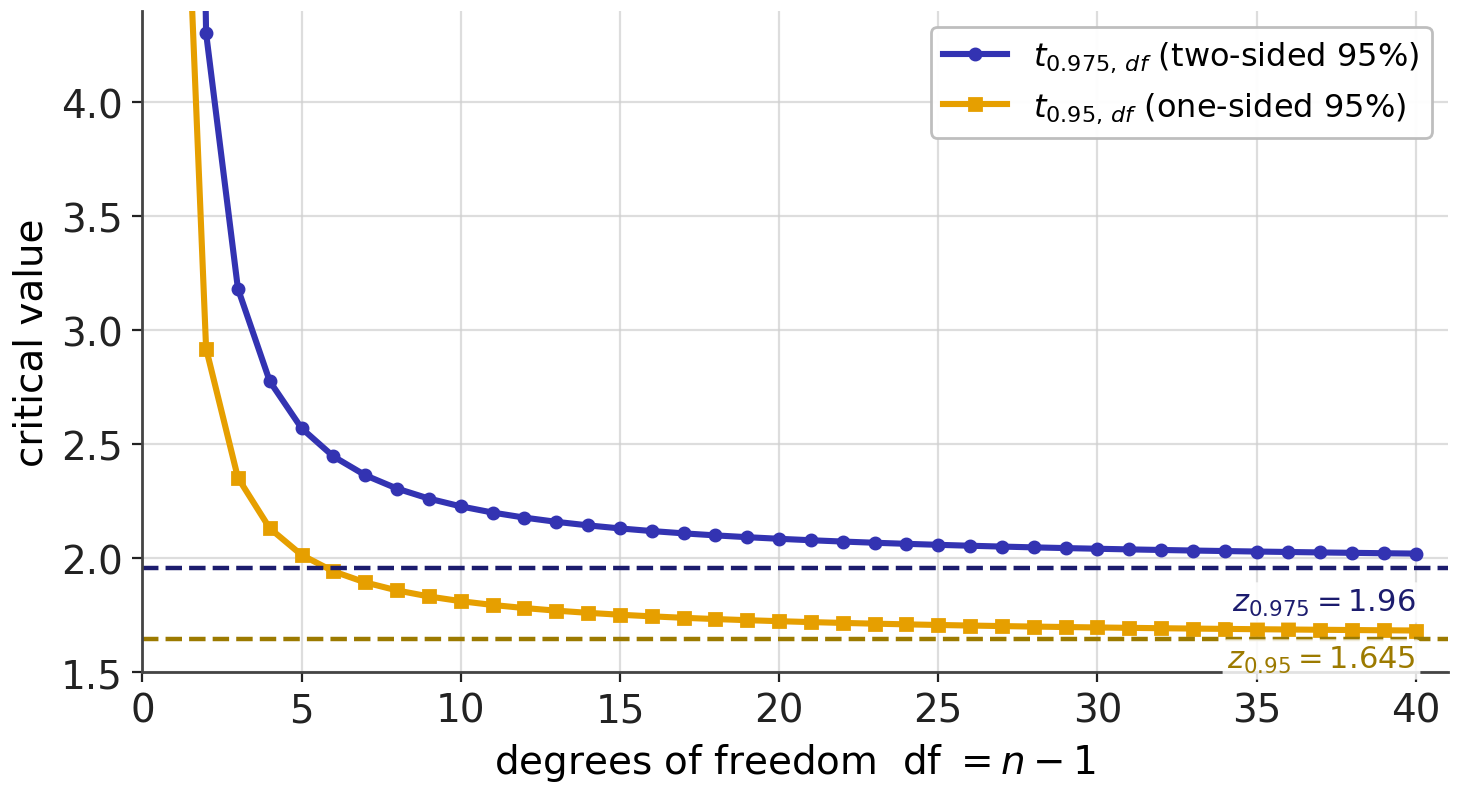
\includegraphics[width=\textwidth,height=0.62\textheight,keepaspectratio]{images/t_crit_convergence.png}
    \end{column}
    \begin{column}{0.36\textwidth}
      \footnotesize
      \begin{itemize}\setlength{\itemsep}{6pt}
        \item Small df $\to$ heavier tails $\to$ \emph{larger} critical value.
        \item As df grows, the $t$-value shrinks towards the $z$-value.
        \item By df $\approx 30$ the gap is tiny -- the $\infty$ row \emph{is}
              the normal.
      \end{itemize}
    \end{column}
  \end{columns}
\end{frame}

\begin{frame}{The wording reveals the test direction}
  \begin{center}
    \renewcommand{\arraystretch}{1.4}
    \begin{tabular}{p{4.6cm}cc}
      \toprule
      \textbf{Signal words} & \textbf{Hypotheses} & \textbf{Direction}\\
      \midrule
      exceed, greater, increased
        & $H_0:\mu=\mu_0$,\ \ $H_1:\mu>\mu_0$ & right-sided\\
      fall below, smaller, reduced
        & $H_0:\mu=\mu_0$,\ \ $H_1:\mu<\mu_0$ & left-sided\\
      \bottomrule
    \end{tabular}
  \end{center}
  \begin{alertblock}{Note}
    The \emph{question} decides one- or two-sided -- not the data. The statement
    you want to find evidence for goes into $H_1$.
  \end{alertblock}
\end{frame}

\begin{frame}{Why put the whole $\alpha$ on one side?}
  \begin{columns}[T]
    \begin{column}{0.60\textwidth}
      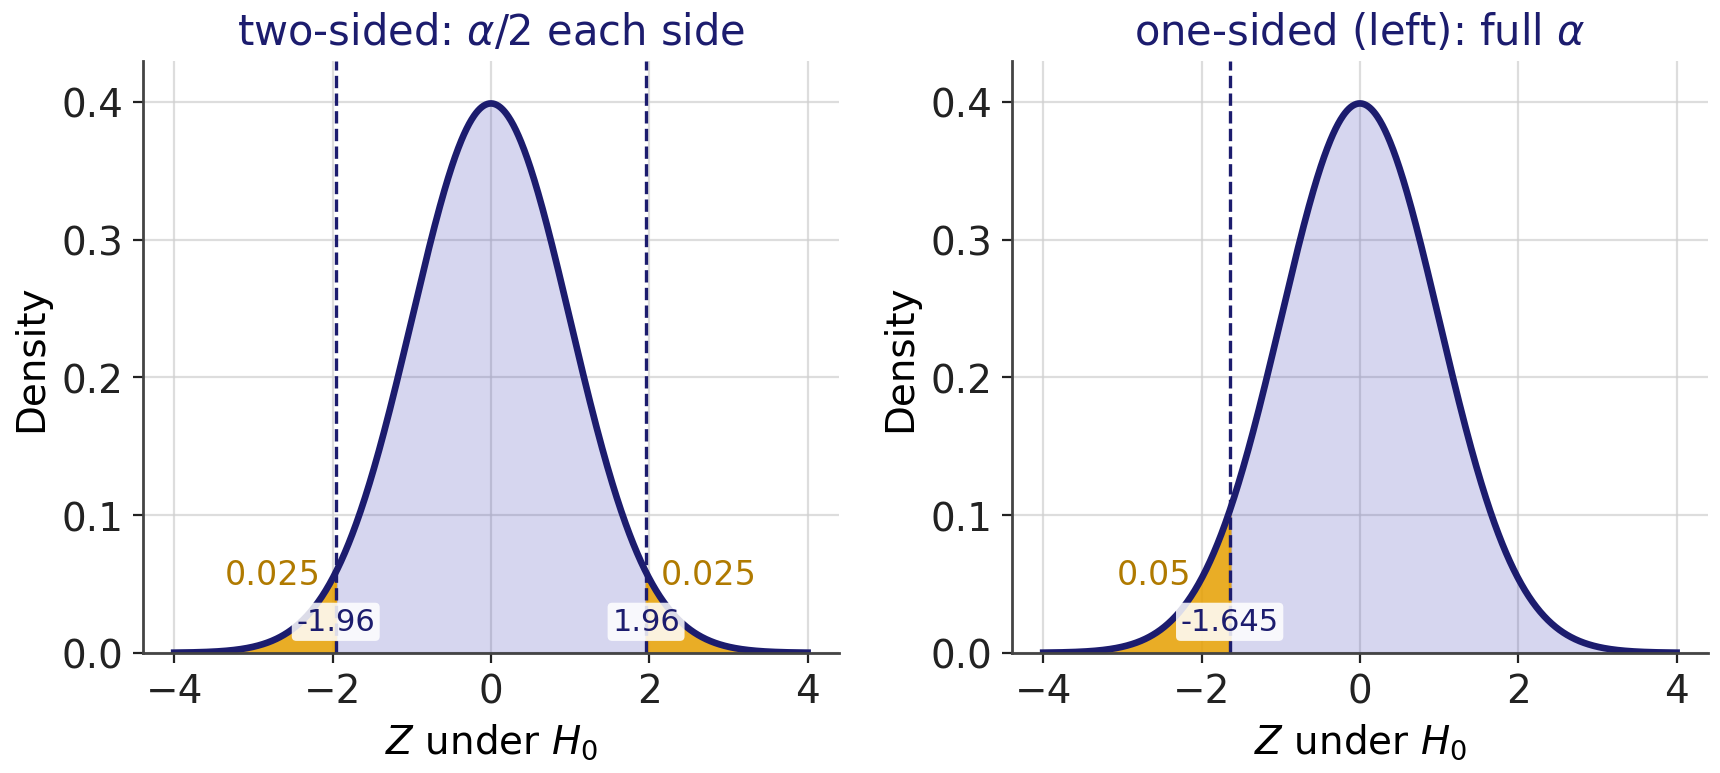
\includegraphics[width=\textwidth,height=0.62\textheight,keepaspectratio]{images/onesided_vs_twosided.png}
    \end{column}
    \begin{column}{0.38\textwidth}
      \footnotesize
      \begin{itemize}\setlength{\itemsep}{4pt}
        \item Two-sided spends $\alpha/2$ guarding \emph{each} tail --
              guarding the harmless side is wasted.
        \item One-sided puts the \emph{whole} $\alpha$ in the relevant tail,
              so the critical value moves inward ($1.96\to1.645$).
        \item A true deviation in that direction now clears the bar
              \emph{more easily}.
      \end{itemize}
    \end{column}
  \end{columns}
  \kernaussage{Same $\alpha$, more power -- but \emph{only} in the chosen
  direction. A one-sided test at level $\alpha$ uses the critical value of a
  two-sided test at level $2\alpha$ on that side.}
\end{frame}
\note{Key sentence to say out loud: ``a one-sided test at $\alpha$ uses the same
cutoff as a two-sided test at $2\alpha$ on that side'' -- that is why $1.96$
drops to $1.645$. Frame it as a trade: more power one way, in exchange for zero
ability to detect the other way.}

\begin{frame}{The price: you must commit in advance}
  \begin{alertblock}{The direction is part of the hypothesis}
    Choose one- vs.\ two-sided \textbf{before} looking at the data -- based on
    the research question alone.
  \end{alertblock}
  \begin{itemize}\setlength{\itemsep}{4pt}
    \item Picking the side \emph{after} seeing which way the data point
          inflates the true Type~I error from $\alpha$ to as much as $2\alpha$.
    \item A one-sided test is \textbf{blind} to deviations in the other
          direction: even a large effect on the ``wrong'' side never rejects
          $H_0$.
    \item If both directions genuinely matter, use a two-sided test.
  \end{itemize}
  \inworten{One-sided tests buy power with a promise -- that the other
  direction really does not matter.}
\end{frame}

\subsection{Left- and right-sided}

\begin{frame}{Left-sided test -- consumer protection}
  \begin{block}{Task}
    A new filling line fills milk (label $1\,\text{l}$). Are the consumer
    protection requirements met, i.e.\ is \emph{not too little} being filled?
    Test with $1-\alpha=0.95$.
  \end{block}
  \begin{itemize}
    \item $H_0:\mu = 1000$ \quad vs.\quad $H_1:\mu < 1000$.
    \item Only $\mu < 1000$ (too little in the bottle) is critical.
  \end{itemize}
  \begin{block}{Procedure}
    Test statistic $T_n = (\bar X - \mu_0)\big/(s/\sqrt n)$; reject if
    $T_n < -t_{1-\alpha,\,n-1}$ \ (known: $Z_n < -z_{1-\alpha}$).\\
    $p$-value: $p = F_{t,n-1}(T_n)$.
  \end{block}
  \inworten{We reject only if $\bar X$ falls \emph{clearly below} $\mu_0$ --
  a value above $\mu_0$ can never be evidence for ``too little''.}
\end{frame}

\begin{frame}{Right-sided test -- do not exceed a limit}
  \begin{block}{Task}
    Advertisement: ``Our milk contains \textbf{at most}
    $1\,\text{mg} = 1000\,\mu\text{g}$ of substance K per litre.'' Is this
    met? We measure in $\mu$g, so $\mu_0 = 1000\,\mu$g.
  \end{block}
  \begin{itemize}
    \item $H_0:\mu = 1000\,\mu\text{g}$ \quad vs.\quad $H_1:\mu > 1000\,\mu\text{g}$.
    \item \emph{Exceeding} the limit is critical.
  \end{itemize}
  \begin{block}{Procedure}
    Reject if $T_n > t_{1-\alpha,\,n-1}$ \ (known: $Z_n > z_{1-\alpha}$).\\
    $p$-value: $p = 1 - F_{t,n-1}(T_n)$.
  \end{block}
  \inworten{Mirror image of the left-sided case: we reject only for values
  \emph{clearly above} $\mu_0$.}
\end{frame}

\begin{frame}{Right-sided test -- substance K with numbers}
  \textbf{Data (known variance):} $\sigma=90\,\mu$g, $n=9$,
  $\bar x = 1060\,\mu$g, $\mu_0=1000$, $\alpha=0.05$, $z_{0.95}=1.645$.
  \begin{align*}
    Z_n &= \frac{1060-1000}{90/\sqrt{9}} = \frac{60}{30} = 2.00\\[2pt]
    Z_n &= 2.00 \;>\; 1.645 = z_{0.95}
  \end{align*}
  \begin{alertblock}{Decision}
    $H_0:\mu=1000$ is \textbf{rejected} ($p = 1-\Phi(2.00) = 0.0228$).
    Evidence that the limit is \emph{exceeded} -- the advertising claim is not
    statistically tenable.
  \end{alertblock}
\end{frame}

\begin{frame}{Left vs.\ right-sided -- at a glance}
  \begin{center}
    \renewcommand{\arraystretch}{1.3}
    \begin{tabular}{>{\raggedright\arraybackslash}p{3.0cm}cc}
      \toprule
       & \textbf{left-sided} & \textbf{right-sided}\\
      \midrule
      Question        & ``too \emph{small}?''      & ``too \emph{large}?''\\
      $H_0$ / $H_1$    & $\mu=\mu_0$ / $\mu<\mu_0$ & $\mu=\mu_0$ / $\mu>\mu_0$\\
      Reject if        & $T_n<-t_{1-\alpha,n-1}$    & $T_n>t_{1-\alpha,n-1}$\\
      Rejection region & far \emph{left} tail       & far \emph{right} tail\\
      $p$-value        & $F_{t,n-1}(T_n)$           & $1-F_{t,n-1}(T_n)$\\
      \bottomrule
    \end{tabular}
  \end{center}
  \footnotesize Some textbooks write the null as $\mu\ge\mu_0$ (left-sided) or
  $\mu\le\mu_0$ (right-sided) -- the test is \textbf{identical}, because critical value and
  $p$-value are computed at the boundary $\mu=\mu_0$ either way.
  \kernaussage{$H_1$ always points \emph{towards} the rejection region: the
  inequality in $H_1$ tells you which tail you reject in.}
\end{frame}
\note{Use this slide as the cheat-sheet. Say: ``the inequality in $H_1$ literally
points at the rejection tail -- $<$ means the left tail, $>$ means the right
tail.'' Quick exercise: have students cover the table and rebuild the reject
rule just from the sign in $H_1$.}

% ---- Quick exercise: right-sided t-test (SfOe Teil 6) ----------------------------
\begin{frame}{Exercise -- discount campaign (right-sided $t$-test)}
  \begin{block}{Problem statement}
    An online shop wants to show that a discount campaign \emph{raises} the
    mean basket value above its previous level of $\mu_0=48$ EUR. A sample of
    $n=25$ orders placed during the campaign gives $\bar x=51.20$ EUR and
    $s=8$ EUR; \ $\alpha=0.05$.
  \end{block}
  \begin{enumerate}\setlength{\itemsep}{3pt}
    \item[a)] State $H_0$ and $H_1$. Which test direction?
    \item[b)] Determine the critical value and the rejection rule.
    \item[c)] Compute $T_n$ and decide.
    \item[d)] From which sample mean $\bar x$ onwards would the shop have
              rejected $H_0$?
  \end{enumerate}
  \textbf{Hint:} $t_{0.95;\,24}=1.7109$.
\end{frame}
\note{Talk track: four minutes. Part d) turns the critical value back into
euros -- the ``critical mean'' $\mu_0+t\cdot\mathrm{SE}$ is the same move as
the acceptance region in the types-of-error section later.}

\begin{frame}{Solution -- discount campaign (right-sided $t$-test)}
  \textbf{Rule:} right-sided: reject $H_0$ if $T_n>t_{1-\alpha;\,n-1}$; \
  $T_n=(\bar x-\mu_0)/(s/\sqrt n)$.
  \begin{itemize}\setlength{\itemsep}{3pt}
    \item[a)] ``raises \ldots\ above'' $\Rightarrow$ $H_0:\mu=48$ \ vs.\ \
          $H_1:\mu>48$ \ (\textbf{right-sided}).
    \item[b)] $\sigma$ unknown $\Rightarrow$ $t$-test, df $=25-1=24$: reject if
          $T_n>t_{0.95;\,24}=\mathbf{1.7109}$.
    \item[c)] $\mathrm{SE}=s/\sqrt n=8/\sqrt{25}=8/5=1.6$; \
          $T_n=\dfrac{51.20-48}{1.6}=\dfrac{3.2}{1.6}=\mathbf{2.00}>1.7109$.
    \item[d)] Solve $T_n>1.7109$ for $\bar x$: \
          $\bar x_{\text{crit}}=\mu_0+t_{0.95;\,24}\cdot\mathrm{SE}
          =48+1.7109\cdot1.6=\mathbf{50.74}$ EUR.
  \end{itemize}
  \begin{alertblock}{Decision}
    $H_0$ is \textbf{rejected}: there is evidence that the campaign raises the
    mean basket value -- any sample mean above $50.74$ EUR would have been
    enough.
  \end{alertblock}
\end{frame}

\subsection{One-sided \texorpdfstring{$p$}{p}-value}

\begin{frame}{One-sided $p$-value -- formulas}
  \begin{columns}[T]
    \begin{column}{0.48\textwidth}
      \begin{block}{Left-sided}
        \[ p = F_{t,n-1}(T_n) \]
        \footnotesize known: $p=\Phi(Z_n)$
      \end{block}
    \end{column}
    \begin{column}{0.48\textwidth}
      \begin{block}{Right-sided}
        \[ p = 1 - F_{t,n-1}(T_n) \]
        \footnotesize known: $p=1-\Phi(Z_n)$
      \end{block}
    \end{column}
  \end{columns}
  \inworten{In a one-sided test we do \emph{not} double -- only the one
  relevant tail area counts.}
\end{frame}

\begin{frame}{One-sided $p$-value -- graphically}
  \begin{center}
    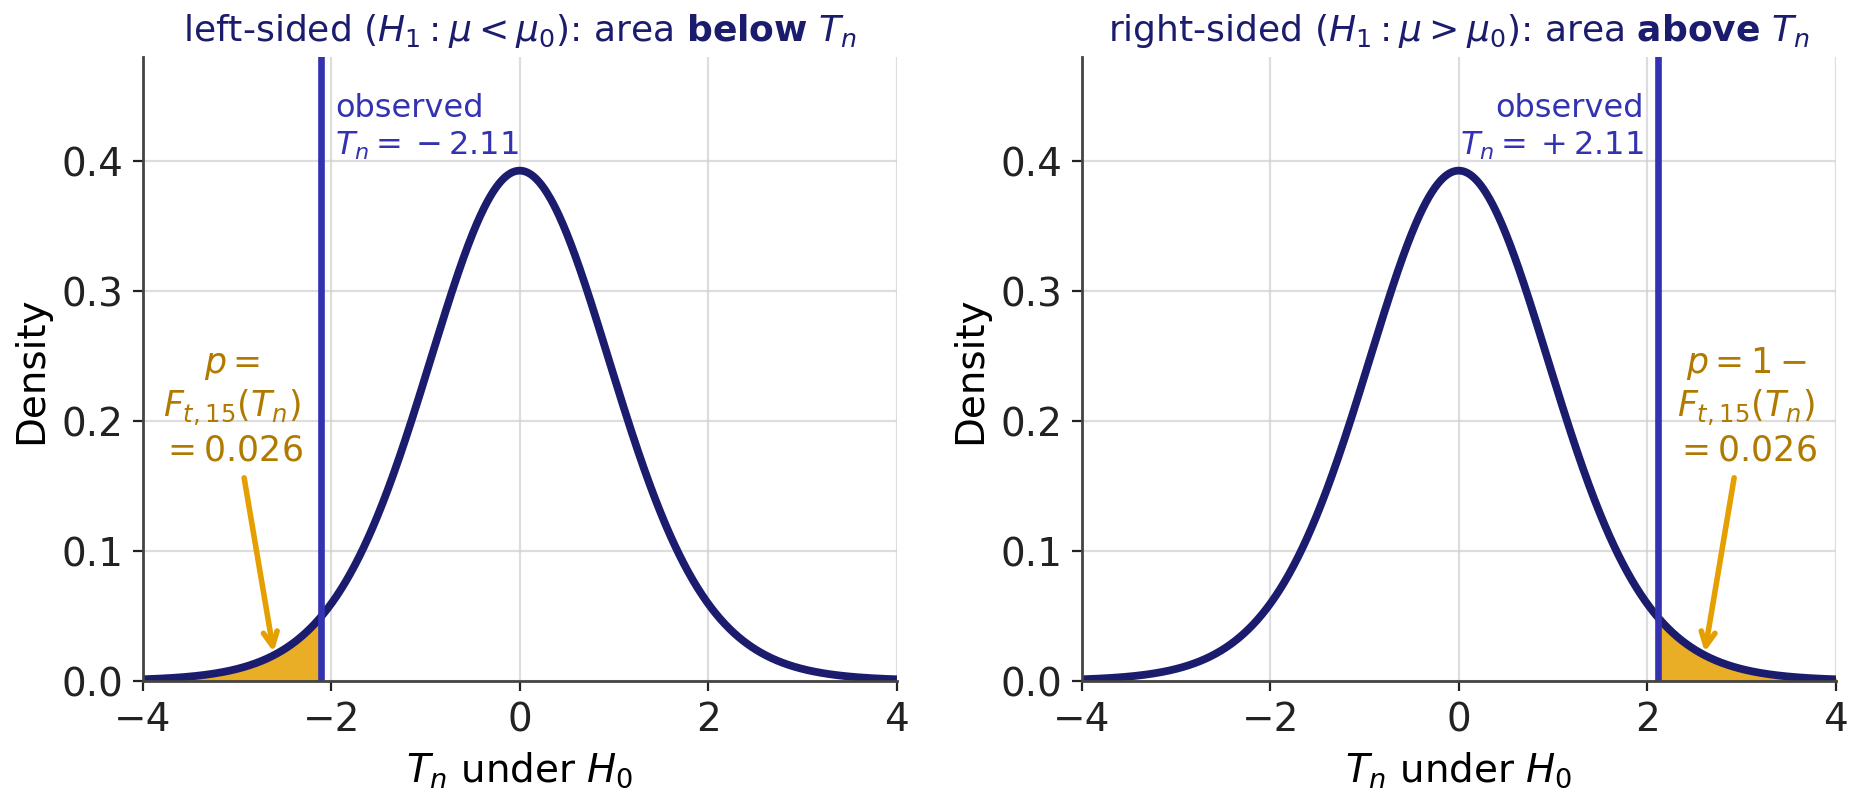
\includegraphics[width=0.97\textwidth,height=0.66\textheight,keepaspectratio]{images/p_value_onesided.png}
  \end{center}
  \footnotesize The $p$-value is the \emph{single} tail area beyond the
  observed statistic, \textbf{in the direction of $H_1$}. Left panel: the
  cream example ($T_n=-2.11$, df $=15$, $p=0.026$).
\end{frame}
\note{Talk track: contrast directly with the two-sided picture (both tails,
factor 2). Here only the tail that $H_1$ points to counts. Ask: ``what would
$p$ be in the LEFT panel if $T_n$ were $+2.11$?'' Answer: $F_{t,15}(2.11)
\approx 0.97$ -- huge, never reject. That sets up the sign-trap slide that
follows.}

\begin{frame}{One-sided $p$-value -- mind the sign}
  \begin{block}{Only the $H_1$-tail counts}
    The one-sided $p$-value is the probability, under $H_0$, of a value
    \emph{at least as far in the $H_1$ direction} as the one observed. The
    opposite tail is irrelevant -- a deviation there supports $H_0$.
  \end{block}
  \begin{alertblock}{Sign check -- a big $|z|$ in the wrong direction is \emph{not} significant}
    Right-sided test with $z=-2.5$: the statistic is on the $H_0$ side, so
    $p = 1-\Phi(-2.5) = 0.994 > 0.5$ -- you \textbf{never} reject, even though
    $|z|$ is large. Check the data point in the $H_1$ direction \emph{before}
    computing.
  \end{alertblock}
  \inworten{Link to two-sided: if the deviation is in the $H_1$ direction,
  $p_{\text{one}} = p_{\text{two}}/2$; otherwise $p_{\text{one}} =
  1-p_{\text{two}}/2$.}
\end{frame}
\note{The classic trap: a right-sided test with a \emph{negative} $T_n$. Say:
``if your statistic is on the $H_0$ side, $p>0.5$ -- stop, you can never
reject.'' Always check the statistic points the $H_1$ way \emph{before}
computing the tail area.}

\begin{frame}{One-sided $p$-value -- milk ($T_n=0.7947$, df $=8$)}
  \begin{columns}[T]
    \begin{column}{0.48\textwidth}
      \begin{block}{Left-sided}
        \[ p = F_{t,8}(0.7947) = 0.7751 \]
        $> 0.05 \Rightarrow H_0:\mu=1000$ kept.
      \end{block}
    \end{column}
    \begin{column}{0.48\textwidth}
      \begin{block}{Right-sided}
        \[ p = 1-0.7751 = 0.2249 \]
        $> 0.05 \Rightarrow H_0:\mu=1000$ kept.
      \end{block}
    \end{column}
  \end{columns}
  \begin{exampleblock}{Interpretation (left)}
    No evidence that the machine fills \emph{too little} -- from a statistical
    point of view, consumer protection is met.
  \end{exampleblock}
\end{frame}

\begin{frame}{One-sided $p$-value -- cream (left, unknown var.)}
  With $T_n = -2.1086$, $\mathrm{df}=15$:
  \[
    p = F_{t,15}(-2.1086) = 0.0261
  \]
  \begin{alertblock}{Decision}
    $p = 0.0261 < 0.05 \Rightarrow H_0:\mu = 250$ is \textbf{rejected}
    (in favour of $H_1:\mu<250$).
  \end{alertblock}
  \kernaussage{In contrast to the two-sided test ($p=0.0522$), the
  left-sided test is \textbf{significant} here -- because the whole $\alpha$
  lies on the critical side.}
\end{frame}

\begin{frame}[fragile]{One-sided test with Python}
\begin{lstlisting}
stats.ttest_1samp(milk, 1000, alternative="less")      # H1: mu < mu0, p = 0.7751
stats.ttest_1samp(milk, 1000, alternative="greater")   # H1: mu > mu0, p = 0.2249

cream = np.array([251, 248, 248, 249, 250, 251, 247, 246,
                  252, 251, 248, 247, 246, 249, 248, 252])
res = stats.ttest_1samp(cream, 250, alternative="less")   # left-sided
ci = res.confidence_interval(0.95)                        # one-sided CI
print(f"t = {res.statistic:.4f}, df = {res.df}, p = {res.pvalue:.4f}")
print(f"95% CI: [{ci.low}, {ci.high:.2f}]")
\end{lstlisting}
  \begin{columns}[T]
    \begin{column}{0.44\textwidth}
      \begin{block}{Cream, left-sided -- output}
\begin{lstlisting}[style=Pyout]
t = -2.1086, df = 15, p = 0.0261
95% CI: [-inf, 249.82]
\end{lstlisting}
      \end{block}
    \end{column}
    \begin{column}{0.52\textwidth}
      \footnotesize The argument \texttt{alternative} controls the
      direction (\texttt{"two-sided"} (default), \texttt{"less"},
      \texttt{"greater"}).
    \end{column}
  \end{columns}
  \trynotebook{section 5.3 ``One-sided $p$-value''}
\end{frame}

\begin{frame}{Exercise -- one- vs.\ two-sided on the same data}
  \begin{block}{Problem statement}
    A coating must \emph{exceed} a target thickness. A test gives
    $T_n = 1.80$ with df $=15$. Compare the right-sided and the two-sided
    decision at $\alpha = 0.05$ -- with the $p$-value and with the critical
    value.
  \end{block}
  \textbf{Hint:} $1-F_{t,15}(1.80) = 0.0460$; \ $t$-table, row df $=15$.
\end{frame}

\begin{frame}{Solution -- one- vs.\ two-sided}
  \textbf{Rule:} one-sided $p$ $=$ the single tail in the $H_1$ direction;
  two-sided $p$ $=$ both tails $=2\times$ the one-sided value (here $T_n$
  points in the $H_1$ direction).
  \begin{align*}
    \text{right-sided:}\ & p = 1-F_{t,15}(1.80) = \mathbf{0.0460} < 0.05
       \;\Rightarrow\; \text{reject}\\
    \text{two-sided:}\ & p = 2\cdot 0.0460 = \mathbf{0.0920} > 0.05
       \;\Rightarrow\; \text{keep}
  \end{align*}
  {\small\textbf{Check with the critical values} ($t$-table, row df $=15$):
  right-sided $T_n=1.80>1.753=t_{0.95;\,15}$ $\Rightarrow$ reject; \
  two-sided $|T_n|=1.80<2.131=t_{0.975;\,15}$ $\Rightarrow$ keep -- the same
  verdicts.\par}
  \kernaussage{Identical data, opposite decisions. The one-sided test is more
  powerful \emph{in the chosen direction} -- exactly why the direction must be
  fixed before seeing the data.}
\end{frame}

\subsection{One-sided confidence intervals}

\begin{frame}{One-sided confidence intervals}
  \begin{itemize}
    \item A one-sided test has a one-sided CI -- only \emph{one} bound, the
          other is $\pm\infty$.
    \item \texttt{scipy} reports them with \texttt{low=-inf} or
          \texttt{high=inf}, i.e.\ $(-\infty;\,x]$ or $[x;\,+\infty)$.
  \end{itemize}
  \begin{block}{Calculation (known variance)}
    \begin{align*}
      \text{left-sided test } (H_1:\mu<\mu_0):\quad &
        \Bigl(-\infty,\ \bar X + z_{1-\alpha}\tfrac{\sigma}{\sqrt n}\Bigr]\\
      \text{right-sided test } (H_1:\mu>\mu_0):\quad &
        \Bigl[\bar X - z_{1-\alpha}\tfrac{\sigma}{\sqrt n},\ +\infty\Bigr)
    \end{align*}
    For unknown variance: replace $z_{1-\alpha}$ by $t_{1-\alpha,\,n-1}$.
  \end{block}
  \footnotesize Note the one-sided quantile $z_{1-\alpha}$ (not $z_{1-\alpha/2}$)
  -- the whole $\alpha$ sits on one side, exactly as in the test.
\end{frame}

\begin{frame}{One-sided CIs -- milk and cream (known)}
  \textbf{CI for the \emph{left-sided} test: upper bound} ($z_{0.95}=1.645$):
  \begin{align*}
    \text{Milk:}\; & 1001 + 1.645\cdot\tfrac{3}{\sqrt{9}} = 1002.645\\
    \text{Cream:}\; & 248.9375 + 1.645\cdot\tfrac{2}{\sqrt{16}} = 249.760
  \end{align*}
  \textbf{CI for the \emph{right-sided} test: lower bound:}
  \begin{align*}
    \text{Milk:}\; & 1001 - 1.645\cdot\tfrac{3}{\sqrt{9}} = 999.355\\
    \text{Cream:}\; & 248.9375 - 1.645\cdot\tfrac{2}{\sqrt{16}} = 248.115
  \end{align*}
  \inworten{If $\mu_0$ lies beyond the single bound, $H_0$ is rejected.}
\end{frame}
\subsection{Exercises}

\begin{frame}{Exercise -- net weight (left-sided, unknown $\sigma$)}
  \begin{block}{Problem statement}
    A package must contain \emph{at least} $\mu_0 = 500\,$g. A sample of
    $n=12$ gives $\bar x = 496$, $s = 6$. Is there evidence of underfilling?
    \ ($\alpha=0.05$.)
  \end{block}
  \textbf{Hint:} $t_{0.95;\,11} = 1.7959$.
\end{frame}

\begin{frame}{Solution -- net weight}
  Underfilling is critical $\Rightarrow$ $H_0:\mu= 500$ vs.\ $H_1:\mu<500$
  (left-sided). Reject if $T_n < -t_{0.95;\,11} = -1.7959$.
  \[
    T_n = \frac{496-500}{6/\sqrt{12}} = \frac{-4}{1.7321} = -2.3094 < -1.7959
  \]
  \begin{alertblock}{Decision}
    Reject $H_0$: evidence of underfilling.
    $p = F_{t,11}(-2.3094) = \mathbf{0.0207} < 0.05$.
  \end{alertblock}
\end{frame}

% ---- Exam-style exercise: muesli (mock exam 3, task 3) ------------------------------
\begin{frame}{Exercise -- muesli filling (exam-style, one-sided $t$-test)}
  \begin{block}{Problem statement}
    A plant fills muesli into packs with target weight $\mu_0=250$\,g.
    Overfilling costs money, so management asks: does the plant fill
    \emph{more} than $250$\,g on average? After maintenance, a sample of
    $n=25$ packs gives $\bar x=252.6$\,g and $s=5.0$\,g; $\alpha=0.05$.\\[2pt]
    {\footnotesize Table values: $t_{0.95;\,24}=1.7109$, $t_{0.975;\,24}=2.0639$,
    $t_{0.99;\,24}=2.4922$, $t_{0.995;\,24}=2.7969$; \ $\Phi(2.60)=0.9953$.}
  \end{block}
  \begin{enumerate}\setlength{\itemsep}{1pt}
    \item[a)] State the hypotheses.
    \item[b)] Compute the standard error, the test statistic and the critical
              value, and decide.
    \item[c)] Which Python command performs this test for a data vector
              \texttt{x}?
    \item[d)] Bracket the $p$-value with the $t$-table, and approximate it with
              the normal distribution.
    \item[e)] Compute the (two-sided) $95\,\%$ CI for $\mu$.
    \item[f)] Decide \emph{without new calculation} whether $H_0:\mu=253$ is
              rejected by a two-sided test at $\alpha=0.05$.
  \end{enumerate}
\end{frame}

\begin{frame}{Solution (1/3) -- muesli: hypotheses and test}
  \textbf{a)} The claim to be established (overfilling) goes into $H_1$
  $\Rightarrow$ \textbf{right-sided}:
  \[
    H_0:\mu=250 \qquad\text{vs.}\qquad H_1:\mu>250
  \]
  \textbf{b)} $\sigma$ unknown $\Rightarrow$ $t$-test with df $=n-1=24$:
  \[
    \frac{s}{\sqrt n}=\frac{5.0}{\sqrt{25}}=\mathbf{1.0\ g},\qquad
    T_n=\frac{252.6-250}{1.0}=\mathbf{2.60},\qquad
    \text{critical value } t_{0.95;\,24}=\mathbf{1.7109}
  \]
  {\small One-sided: the \emph{whole} $\alpha$ sits in the right tail, so the
  $0.95$-quantile (not $0.975$).}
  \begin{alertblock}{Decision}
    $T_n=2.60>1.7109$ $\Rightarrow$ $H_0$ is \textbf{rejected}: the plant fills
    significantly more than $250$\,g on average -- it should be readjusted.
  \end{alertblock}
\end{frame}

\begin{frame}[fragile]{Solution (2/3) -- muesli: Python and the $p$-value}
  \textbf{c)} and the exact $p$-value from the summary figures:
\begin{lstlisting}
from scipy import stats
# raw data x available:  stats.ttest_1samp(x, popmean=250, alternative="greater")
t = (252.6 - 250) / (5.0 / 25 ** 0.5)                  # from the summary figures
print(f"{t:.2f} {stats.t.sf(t, df=24):.4f} {stats.norm.sf(t):.4f}")
\end{lstlisting}
  \vspace{-4pt}
\begin{lstlisting}[style=Pyout]
2.60 0.0079 0.0047
\end{lstlisting}
  \textbf{d)} $T_n$ lies between the $0.99$- and the $0.995$-quantile:
  \[
    t_{0.99;\,24}=2.4922 \;<\; 2.60 \;<\; 2.7969=t_{0.995;\,24}
    \;\Longrightarrow\; \mathbf{0.005<p<0.01}
  \]
  {\small One-sided: the upper-tail areas $0.01$ and $0.005$ \emph{are} the
  bounds -- no doubling (exact: $p=0.0079$).}\\[2pt]
  Normal approximation: $p\approx1-\Phi(2.60)=1-0.9953=\mathbf{0.0047}$ --
  smaller than the exact $0.0079$, because the $t$-distribution has heavier
  tails. Both are far below $0.05$: same decision.
  \trynotebook{section 5.5 ``Exercises''}
\end{frame}

\begin{frame}{Solution (3/3) -- muesli: CI and duality}
  \[
    \text{\textbf{e)}}\quad 252.6\pm2.0639\cdot1.0=252.6\pm2.0639
    \ \Rightarrow\ \text{CI}_{0.95}=\mathbf{[\,250.54\,;\,254.66\,]}\ \text{g}
  \]
  \textbf{f)} The two-sided CI contains exactly the values $\mu_0$ that a
  two-sided test does \emph{not} reject:
  \[
    250.54<253<254.66 \ \Rightarrow\ H_0:\mu=253 \text{ is \textbf{not} rejected.}
  \]
  {\small Every $\mu_0<250.54$ or $\mu_0>254.66$ would be rejected -- e.g.\
  $\mu_0=250$.}
  \begin{alertblock}{Careful with the duality}
    The \emph{two-sided} CI belongs to the \emph{two-sided} test. The partner
    of the right-sided test in b) is the one-sided CI
    $[\,252.6-1.7109\cdot1.0\,;\,\infty)=[\,250.89\,;\,\infty)$ -- it excludes
    $250$, consistent with the rejection.
  \end{alertblock}
\end{frame}
\note{Talk track: typical exam errors in this task -- $t_{0.975}$ instead of
$t_{0.95}$ for a one-sided test; doubling the one-sided $p$-value; swapping
the bracket ($t_{0.99}$ belongs to a tail area of $0.01$, not $0.99$);
df $=25$ instead of $24$. The normal approximation shows nicely why the
$t$-tails are heavier.}

% ---- Exam-style exercise: delivery time revisited (mock exam 6, task 3A) ----------
\begin{frame}{Exercise -- delivery time revisited (one-sided test vs.\ two-sided CI)}
  \begin{block}{Problem statement}
    The logistics provider from the delivery-time exercise now advertises a
    mean delivery time \emph{below} $\mu_0=48$ hours. A new sample of $n=16$
    shipments gives $\bar x=46.4$\,h and $s=3.2$\,h; $\alpha=0.05$.\\[2pt]
    {\footnotesize Table values: $t_{0.95;\,15}=1.7531$, $t_{0.975;\,15}=2.1314$.}
  \end{block}
  \begin{enumerate}\setlength{\itemsep}{2pt}
    \item[a)] State the hypotheses and carry out the test with the critical
              value.
    \item[b)] Compute the two-sided $95\,\%$ CI. Does it contain $48$? Is that
              a contradiction to a)?
    \item[c)] Which confidence interval matches the test in a)? Compute it.
    \item[d)] Check a) and c) with Python.
  \end{enumerate}
\end{frame}

\begin{frame}{Solution (1/2) -- delivery time revisited: left-sided test}
  \textbf{a)} The advertised claim goes into $H_1$ $\Rightarrow$
  \textbf{left-sided}:
  \[
    H_0:\mu=48 \qquad\text{vs.}\qquad H_1:\mu<48
  \]
  \[
    \frac{s}{\sqrt n}=\frac{3.2}{\sqrt{16}}=0.8,\qquad
    T_n=\frac{46.4-48}{0.8}=\mathbf{-2.00},\qquad
    \text{critical value: }{-t_{0.95;\,15}}=\mathbf{-1.7531}
  \]
  \begin{alertblock}{Decision}
    $T_n=-2.00<-1.7531$ $\Rightarrow$ $H_0$ is \textbf{rejected}
    ($p=F_{t,15}(-2.00)=0.0320$): the mean delivery time is significantly
    below $48$\,h -- the advertisement is statistically supported.
  \end{alertblock}
  {\small The negative sign belongs to the result: the rejection region lies on
  the \emph{left}. Comparing absolute values would lose the direction.}
\end{frame}

\begin{frame}[fragile]{Solution (2/2) -- delivery time revisited: which CI?}
  \textbf{b)} $46.4\pm2.1314\cdot0.8=46.4\pm1.7051$ $\Rightarrow$
  $\text{CI}_{0.95}=\mathbf{[\,44.69\,;\,48.11\,]}$ -- it \emph{contains}
  $48$! \emph{No} contradiction: the two-sided CI belongs to the
  \emph{two-sided} test, which would indeed keep $H_0$ here ($p=0.064$). The
  one-sided test puts the whole $\alpha$ on one side and is sharper in that
  direction.\\[3pt]
  \textbf{c)} The partner of the left-sided test is the one-sided CI with an
  upper bound:
  \[
    \Bigl(-\infty\,;\ 46.4+1.7531\cdot0.8\Bigr]=\mathbf{(-\infty\,;\,47.80]}
    \quad\Rightarrow\quad 48\ \text{lies outside -- consistent with a).}
  \]
  \textbf{d)} \vspace{-6pt}
\begin{lstlisting}
from scipy import stats
t = (46.4 - 48) / (3.2 / 16 ** 0.5)
print(f"{t:.2f} {stats.t.cdf(t, df=15):.4f}")           # T_n, left-sided p-value
print(f"{46.4 + stats.t.ppf(0.95, df=15) * 0.8:.2f}")   # upper bound of one-sided CI
\end{lstlisting}
  \vspace{-4pt}
  \begin{columns}[T]
    \begin{column}{0.22\textwidth}
\begin{lstlisting}[style=Pyout]
-2.00 0.0320
47.80
\end{lstlisting}
    \end{column}
    \begin{column}{0.74\textwidth}
      \footnotesize With raw data: \texttt{stats.ttest\_1samp(x, 48,
      alternative="less")} and \texttt{.confidence\_interval(0.95)}.
    \end{column}
  \end{columns}
  \trynotebook{section 5.5 ``Exercises''}
\end{frame}
\note{Talk track: the punchline of this task is the duality rule ``like with
like'': one-sided test $\leftrightarrow$ one-sided CI, two-sided test
$\leftrightarrow$ two-sided CI. Ask the room before showing b): ``the test
rejected 48 -- will the 95\,\% CI exclude 48?'' Many say yes. It is the
compact version of the earlier ``one- vs.\ two-sided on the same data''
exercise.}

% ============================================================================
% SECTION 6: TYPES OF ERROR
% ============================================================================
\section[Errors]{Types of Error}

\subsection{The two types of error}

\begin{frame}{Two ways to be wrong}
  \begin{block}{Intuition}
    Like a smoke detector, we can be wrong in two ways:
    \textbf{false alarm} or \textbf{missed fire}.
  \end{block}
  \begin{center}
    \renewcommand{\arraystretch}{1.5}
    \begin{tabular}{lcc}
      \toprule
       \textbf{Decision} & \textbf{$H_0$ true} & \textbf{$H_0$ false}\\
      \midrule
      reject $H_0$
        & \cellcolor{hsbirot!20}\,Type I error ($\alpha$)\,
        & \cellcolor{green!18}\,correct (power $1-\beta$)\,\\
      keep $H_0$
        & \cellcolor{green!18}\,correct ($1-\alpha$)\,
        & \cellcolor{hsbiorange!28}\,Type II error ($\beta$)\,\\
      \bottomrule
    \end{tabular}
  \end{center}
  \footnotesize \textbf{Type I error} = false alarm (reject although $H_0$ is
  true). \quad \textbf{Type II error} = miss (keep although $H_1$ is true).
\end{frame}
\note{Talk track: build the table column by column -- ``first fix the TRUE
state of the world (column), then look at what our test DID (row).'' Smoke
detector: too sensitive = many false alarms (Type I); too sluggish = missed
fire (Type II). Make students say which error the milk test could have made
(it kept $H_0$, so only a Type II is possible). Common confusion: thinking
both errors can occur in the same test run -- only one column is ever real.}

\begin{frame}{$\alpha$ and $\beta$ in a picture}
  \begin{columns}[T]
    \begin{column}{0.62\textwidth}
      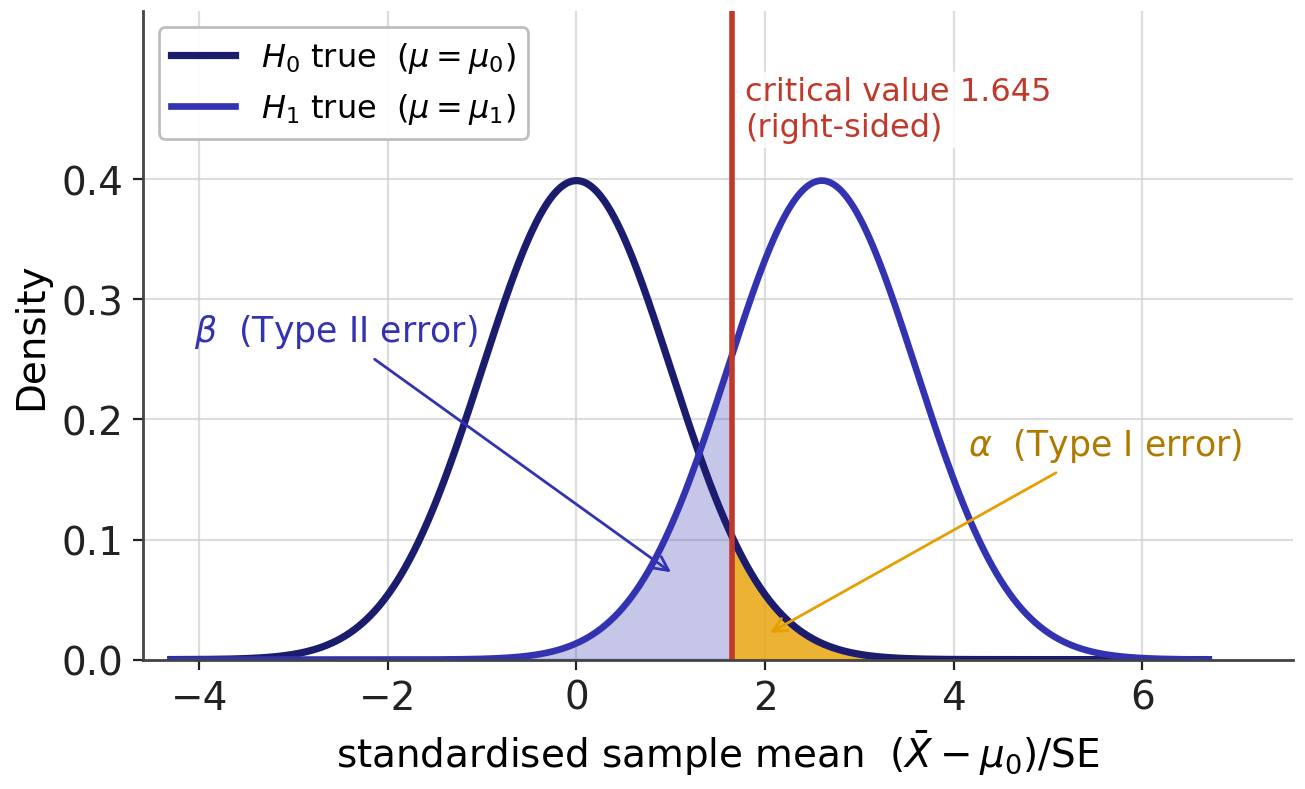
\includegraphics[width=\textwidth,height=0.64\textheight,keepaspectratio]{images/error_alpha_beta.png}
    \end{column}
    \begin{column}{0.36\textwidth}
      \footnotesize
      \begin{itemize}\setlength{\itemsep}{4pt}
        \item The two curves show the \emph{standardised} $\bar X$ in each
              ``world'': left centred at $\mu_0$ (value $0$, if $H_0$ holds),
              right at the true $\mu_1$ (here $2.6$ standard errors above
              $\mu_0$, if $H_1$); the red line is the critical value of a
              right-sided test ($1.645$).
        \item \textcolor{hsbiorange!85!black}{$\alpha$}: $H_0$ true, but
              beyond the critical value.
        \item \textcolor{hsbiblau}{$\beta$}: $H_1$ true, but on this side.
        \item The distributions overlap -- both errors cannot be $0$ at once.
      \end{itemize}
    \end{column}
  \end{columns}
\end{frame}

\subsection{\texorpdfstring{$\alpha$, $\beta$}{alpha, beta} and power}

\begin{frame}{Type I error ($\alpha$) -- controllable}
  \begin{block}{Definition}
    \[
      P(\text{reject } H_0 \mid H_0 \text{ true}) = \alpha
    \]
  \end{block}
  \begin{itemize}
    \item \textbf{Directly controllable} through the choice of $\alpha$
          (typically $0.05$).
    \item In $5\,\%$ of cases a \emph{true} $H_0$ is wrongly rejected.
  \end{itemize}
  \begin{exampleblock}{Milk}
    $H_0:\mu=1000$ is true, yet the test rejects (false alarm) --
    probability $=\alpha$.
  \end{exampleblock}
\end{frame}

\begin{frame}{Type II error ($\beta$) -- only indirectly influenced}
  \begin{block}{Definition (at a specific alternative $\mu_1$)}
    \[
      P(\text{keep } H_0 \mid \mu = \mu_1) = \beta
    \]
  \end{block}
  \begin{itemize}\setlength{\itemsep}{2pt}
    \item No \emph{direct} lever; $\beta$ depends on:
          \begin{itemize}\footnotesize
            \item $\alpha$, sample size $n$, spread $\sigma^2$,
            \item true deviation $|\mu-\mu_0|$ (effect size).
          \end{itemize}
    \item At a fixed $\mu_1$: smaller $\alpha$ $\Rightarrow$ higher bar
          $\Rightarrow$ more misses ($\beta$ \emph{rises}); \ larger $n$
          $\Rightarrow$ smaller SE $\Rightarrow$ $\beta$ \emph{falls}.
  \end{itemize}
  \kernaussage{Power $=1-\beta$: the ability to actually reject a
  \emph{false} $H_0$.}
\end{frame}

\begin{frame}{Only one error is controllable}
  \textbf{Question:} Which error can we only make when we \emph{reject} $H_0$?
  \begin{block}{Answer}
    The Type I error -- and that is exactly the one we control via $\alpha$.
  \end{block}
  \begin{alertblock}{Consequence for the choice of hypotheses}
    This is why the claim you want to \emph{establish} goes into $H_1$ (rule of
    thumb from above): wrongly declaring it ``established'' -- rejecting $H_0$
    although $H_0$ holds -- is the costly mistake, and exactly this one is the
    controllable Type~I error.
  \end{alertblock}
\end{frame}

\begin{frame}{Trade-off and power}
  \begin{columns}[T]
    \begin{column}{0.6\textwidth}
      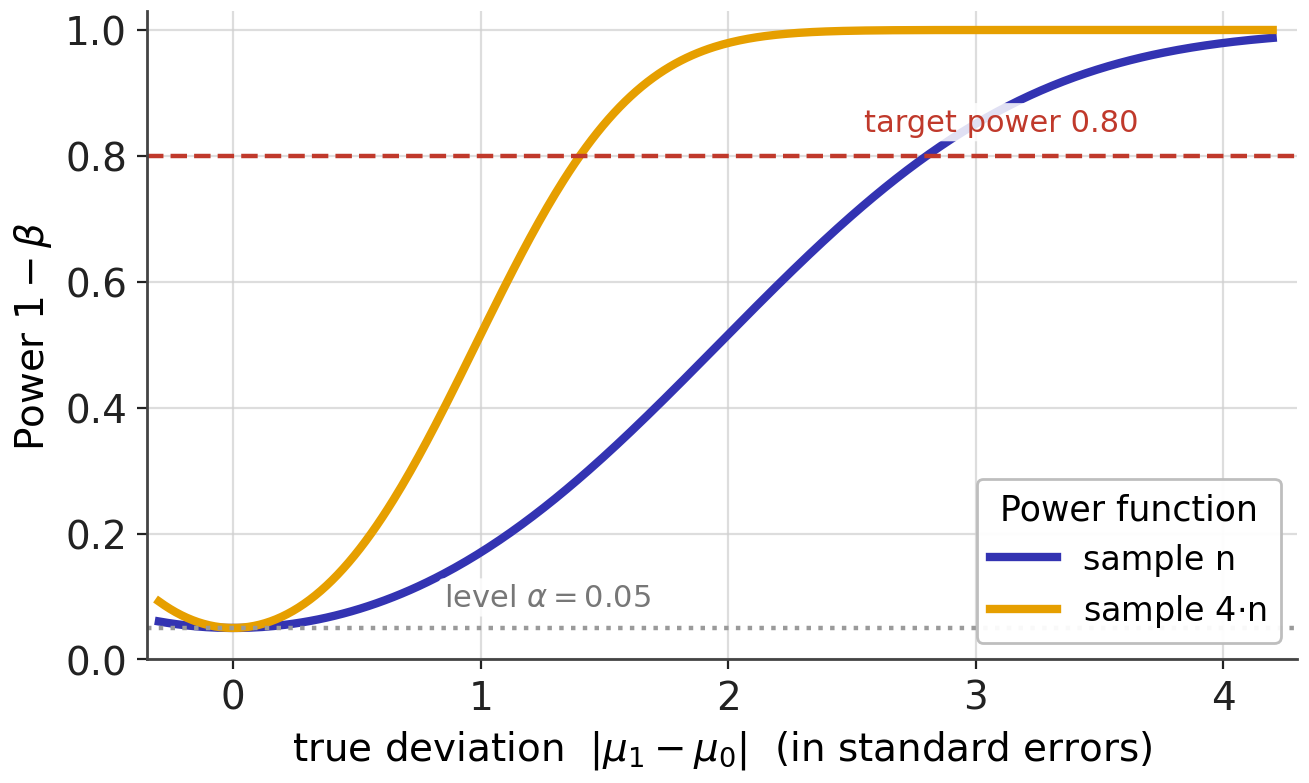
\includegraphics[width=\textwidth,height=0.6\textheight,keepaspectratio]{images/power_curve.png}
    \end{column}
    \begin{column}{0.38\textwidth}
      \footnotesize
      \begin{itemize}\setlength{\itemsep}{4pt}
        \item $\alpha\!\downarrow \Rightarrow \beta\!\uparrow$ (trade-off).
        \item Larger $n$ raises power at every $\mu\neq\mu_0$ (at $\mu_0$ it
              stays at $\alpha$) -- more power at the same level.
        \item Power rises with the true deviation.
      \end{itemize}
    \end{column}
  \end{columns}
  \begin{block}{Practice}
    Typically $\alpha=0.05$ and desired power $1-\beta\ge 0.80$. A
    \textbf{power analysis} provides the required $n$.
  \end{block}
\end{frame}

\begin{frame}{Computing $\beta$ concretely -- milk}
  \textbf{Setup:} $H_0:\mu=1000$ vs.\ $H_1:\mu\neq1000$, $\sigma=3$, $n=9$
  ($\mathrm{SE}=1$), $\alpha=0.05$.\\[2pt]
  \textbf{Step 1} -- turn ``$|Z_n|\le1.96$'' into bounds on $\bar X$:
  $\mu_0\pm1.96\cdot\mathrm{SE}=1000\pm1.96=[998.04\,;\,1001.96]$.\\[2pt]
  \textbf{Step 2} -- the truth is $\mu_1=1002$; find how often $\bar X$ still
  lands in that region, \emph{standardising with $\mu_1$}:
  \begin{align*}
    \beta &= P\bigl(998.04 \le \bar X \le 1001.96 \;\big|\; \mu=1002\bigr)\\
          &= \Phi\!\bigl(\tfrac{1001.96-1002}{1}\bigr) - \Phi\!\bigl(\tfrac{998.04-1002}{1}\bigr)
           = 0.484
  \end{align*}
  \begin{exampleblock}{Result}
    Power $=1-\beta = 0.516$: a true deviation of $2\,$ml is detected with
    $n=9$ in only just over half the cases.
  \end{exampleblock}
\end{frame}
\note{Talk track: the key move is the change of world. Step 1 lives in the
$H_0$ world (where the acceptance region was built); step 2 asks how often
$\bar X$ lands in that same region when the TRUTH is $\mu_1=1002$ -- so we
standardise with $1002$, not $1000$. Students often reuse $\mu_0$ in step 2;
catch that explicitly. The sobering message: with $n=9$, a real 2\,ml error
escapes detection almost half the time.}

\begin{frame}{Four levers for more power}
  More sample size helps decisively. Same situation with $n=36$ instead of $9$:
  \[
    \text{SE}=\tfrac{3}{\sqrt{36}}=0.5 \;\Rightarrow\; \beta = 0.021,\quad
    \text{power}=0.979.
  \]
  \begin{block}{Levers of power $1-\beta$}
    \begin{enumerate}
      \item \textbf{Sample size} $n\uparrow$ (strongest lever).
      \item \textbf{Effect size} $|\mu_1-\mu_0|$ (given).
      \item \textbf{Spread} $\sigma\downarrow$ (e.g.\ measure more precisely).
      \item \textbf{Level} $\alpha\uparrow$ (buys more Type I error).
    \end{enumerate}
  \end{block}
  \kernaussage{Quadrupling $n$ from $9$ to $36$ raises the power from
  $0.52$ to $0.98$.}
\end{frame}
\note{Talk track: go through the four levers and ask for each ``who controls
this?'' -- $n$: the researcher (budget); effect size: nature/the question;
$\sigma$: partly the lab (better instruments); $\alpha$: the convention, and
raising it is usually unacceptable. So in practice power planning $=$ sample
size planning. Connect back to the CI length slide: same logic,
$1/\sqrt n$.}

% ---- beta and power with Python ----------------------------------------------------
\begin{frame}[fragile]{$\beta$ and power with Python}
\begin{lstlisting}
import numpy as np
from scipy import stats
from statsmodels.stats.power import NormalIndPower
for n in (9, 36):                        # milk: mu0 = 1000, true mu1 = 1002, sigma = 3
    se = 3 / np.sqrt(n)
    lo, hi = 1000 - 1.96 * se, 1000 + 1.96 * se         # acceptance region (H0 world)
    beta = stats.norm.cdf(hi, 1002, se) - stats.norm.cdf(lo, 1002, se)  # mu1 world
    print(f"n = {n}: beta = {beta:.3f}, power = {1 - beta:.3f}")
pw = NormalIndPower()                    # power of the z-test; ratio=0: one sample
pw.power(effect_size=2/3, nobs1=9, alpha=0.05, ratio=0)              # 0.516
pw.solve_power(effect_size=2/3, power=0.80, alpha=0.05, ratio=0)     # 17.66 -> n = 18
\end{lstlisting}
  \begin{columns}[T]
    \begin{column}{0.44\textwidth}
      \begin{block}{Output}
\begin{lstlisting}[style=Pyout]
n = 9: beta = 0.484, power = 0.516
n = 36: beta = 0.021, power = 0.979
\end{lstlisting}
      \end{block}
    \end{column}
    \begin{column}{0.52\textwidth}
      \footnotesize Effect size $d=|\mu_1-\mu_0|/\sigma=2/3$.
      \texttt{solve\_power} does the power analysis: $80\,\%$ power needs
      at least $n=18$ bottles.
    \end{column}
  \end{columns}
  \trynotebook{section 6.2 ``$\alpha$, $\beta$ and power''}
\end{frame}
\subsection{Exercises}

\begin{frame}{Exercise -- compute $\beta$ and power (two-sided)}
  \begin{block}{Problem statement}
    Test $H_0:\mu = 100$ vs.\ $H_1:\mu\neq 100$, known $\sigma = 10$, $n=25$,
    $\alpha=0.05$. The true mean is actually $\mu_1 = 105$. Find the Type~II
    error $\beta$ and the power.
  \end{block}
  \textbf{Step 1:} the acceptance region for $\bar X$ under $H_0$.
\end{frame}

\begin{frame}{Solution -- $\beta$ and power (two-sided)}
  $\text{SE} = 10/\sqrt{25} = 2$. Acceptance region:
  $100 \pm 1.96\cdot 2 = [96.08\,;\,103.92]$.
  \begin{align*}
    \beta &= P(96.08 \le \bar X \le 103.92 \mid \mu = 105)\\
          &= \Phi\!\Big(\tfrac{103.92-105}{2}\Big)
             - \Phi\!\Big(\tfrac{96.08-105}{2}\Big)
           = \Phi(-0.54) - \Phi(-4.46)\\
          &= 0.2946 - 0.0000 = \mathbf{0.2946}
  \end{align*}
  \begin{exampleblock}{Power}
    $1-\beta = \mathbf{0.7054}$: a true shift of $5$ units is detected in about
    $71\,\%$ of samples.
  \end{exampleblock}
\end{frame}

\begin{frame}{Exercise -- power of a one-sided test}
  \begin{block}{Problem statement}
    Now use a \emph{right-sided} test, $H_1:\mu>100$, with $\sigma=10$,
    $n=25$, $\alpha=0.05$, true $\mu_1=105$. Find the power and compare with
    the two-sided value $0.7054$.
  \end{block}
\end{frame}

\begin{frame}{Solution -- one-sided power}
  $\text{SE}=2$. Critical mean:
  $\bar x_{\text{crit}} = 100 + 1.645\cdot 2 = 103.29$.
  \[
    1-\beta = P(\bar X > 103.29 \mid \mu=105)
            = 1-\Phi\!\Big(\tfrac{103.29-105}{2}\Big)
            = 1-\Phi(-0.855) = \mathbf{0.8037}
  \]
  \begin{exampleblock}{Comparison}
    Power $0.804$ vs.\ $0.705$ two-sided -- the one-sided test is \emph{more
    powerful} for the same $n$ and $\alpha$, because the whole $\alpha$ sits on
    the relevant side.
  \end{exampleblock}
\end{frame}

% ============================================================================
% SECTION 7: SUMMARY
% ============================================================================
\section[Summary]{Summary}

\begin{frame}{Summary 1 -- foundations}
  \begin{columns}[T]
    \begin{column}{0.48\textwidth}
      \begin{block}{Normal distribution}
        $X\sim N(\mu,\sigma^2)$ \ $\Rightarrow$ \
        $Z=\dfrac{X-\mu}{\sigma}\sim N(0,1)$\\[4pt]
        $P(X\le x)=\Phi\bigl(\tfrac{x-\mu}{\sigma}\bigr)$, \quad
        $\Phi(-z)=1-\Phi(z)$\\[4pt]
        quantile: $x_p=\mu+\sigma\,z_p$, \quad $z_{0.975}=1.96$
      \end{block}
    \end{column}
    \begin{column}{0.48\textwidth}
      \begin{block}{Sampling distribution of $\bar X$}
        $E(\bar X)=\mu$, \quad $\mathrm{Var}(\bar X)=\sigma^2/n$, \quad
        $\mathrm{SE}=\sigma/\sqrt n$\\[4pt]
        normal data: $\bar X\sim N(\mu,\sigma^2/n)$ exactly;\\[2pt]
        otherwise (CLT, $n\gtrsim30$): approximately.
      \end{block}
    \end{column}
  \end{columns}
  \kernaussage{Every interval and test in this part \emph{standardises}
  $\bar X$ with its standard error -- and the CLT makes this work even for
  non-normal data.}
\end{frame}

\begin{frame}{Summary 2 -- confidence intervals}
  \begin{block}{Known variance $\sigma$ \quad ($Z_n\sim N(0,1)$)}
    \[
      \text{CI}_{1-\alpha} =
      \left[\bar{X}-z_{1-\alpha/2}\frac{\sigma}{\sqrt{n}},\;
            \bar{X}+z_{1-\alpha/2}\frac{\sigma}{\sqrt{n}}\right]
    \]
  \end{block}
  \begin{block}{Unknown variance \quad ($T_n\sim t_{n-1}$)}
    \[
      \text{CI}_{1-\alpha} =
      \left[\bar{X}-t_{1-\alpha/2,\,n-1}\frac{s}{\sqrt{n}},\;
            \bar{X}+t_{1-\alpha/2,\,n-1}\frac{s}{\sqrt{n}}\right]
    \]
  \end{block}
  \textbf{Sample size} for a margin of error $e$ (known $\sigma$):
  \ $n\ge\bigl(z_{1-\alpha/2}\,\sigma/e\bigr)^2$, rounded up.
\end{frame}

\begin{frame}{Summary 3 -- hypothesis test (two-sided)}
  $H_0:\mu=\mu_0$ vs.\ $H_1:\mu\ne\mu_0$
  \begin{block}{Test statistics}
    \[
      Z_n = \frac{\bar{X}-\mu_0}{\sigma/\sqrt{n}}\sim N(0,1),\qquad
      T_n = \frac{\bar{X}-\mu_0}{s/\sqrt{n}}\sim t_{n-1}
      \qquad(\text{under } H_0)
    \]
  \end{block}
  \begin{alertblock}{Decision}
    Reject if $|Z_n|>z_{1-\alpha/2}$ ($\sigma$ known) or
    $|T_n|>t_{1-\alpha/2,\,n-1}$ ($\sigma$ unknown).
  \end{alertblock}
\end{frame}

\begin{frame}{Summary 4 -- the $p$-value}
  \begin{block}{One idea behind every formula}
    $p$ = probability, \emph{if $H_0$ were true}, of a value \textbf{at least as
    extreme as observed} -- in the direction(s) that $H_1$ allows.
  \end{block}
  \begin{center}
    \renewcommand{\arraystretch}{1.4}
    \begin{tabular}{>{\raggedright\arraybackslash}p{2.6cm}>{\raggedright\arraybackslash}p{4.2cm}c}
      \toprule
      \textbf{If $H_1$ is\ldots} & \textbf{add up the\ldots} & \textbf{$p$ \ (unknown $\sigma$)}\\
      \midrule
      $\mu\neq\mu_0$ & \emph{both} tails beyond $|T_n|$ & $2\,F_{t,n-1}(-|T_n|)$\\
      $\mu<\mu_0$ (left)  & \emph{lower} tail below $T_n$ & $F_{t,n-1}(T_n)$\\
      $\mu>\mu_0$ (right) & \emph{upper} tail above $T_n$ & $1-F_{t,n-1}(T_n)$\\
      \bottomrule
    \end{tabular}
  \end{center}
  \footnotesize \textbf{Known $\sigma$?} Just replace $T_n\to Z_n$ and
  $F_{t,n-1}\to\Phi$. \quad \textbf{Decide:} $p<\alpha \Rightarrow$ reject $H_0$.
\end{frame}

\begin{frame}{Summary 5 -- one-sided tests \& types of error}
  \begin{block}{One-sided tests (unknown variance)}
    \begin{tabular}{ll}
      \textbf{left:}\ \ \, $H_1:\mu<\mu_0$ & reject if $T_n<-t_{1-\alpha,\,n-1}$\\[2pt]
      \textbf{right:}\ $H_1:\mu>\mu_0$ & reject if $T_n> t_{1-\alpha,\,n-1}$
    \end{tabular}
  \end{block}
  \begin{block}{Types of error}
    $P(\text{reject } H_0\mid \mu=\mu_0)= \alpha$ \quad
    $P(\text{keep } H_0\mid \mu=\mu_1)= \beta$ \\
    $\alpha$ is \emph{controllable}; $\beta$ falls with $n\uparrow$ and $\alpha\uparrow$;
    power $=1-\beta$.
  \end{block}
\end{frame}

\begin{frame}[fragile]{Summary 6 -- important Python commands}
  \begin{columns}[T]
    \begin{column}{0.46\textwidth}
      \begin{block}{Distributions}
\begin{lstlisting}
from scipy import stats
stats.norm.cdf(1.96)          # Phi(z)
stats.norm.sf(1.96)           # 1 - Phi(z)
stats.norm.ppf(0.975)         # z_p
stats.norm.cdf(997, 1000, 3)  # P(X<=x)
stats.t.cdf(-2.11, df=15)     # F_t,df(t)
stats.t.ppf(0.975, df=8)      # t_p,df
\end{lstlisting}
      \end{block}
    \end{column}
    \begin{column}{0.52\textwidth}
      \begin{block}{Tests, intervals, sample size}
\begin{lstlisting}
res = stats.ttest_1samp(x, popmean=1000)
res = stats.ttest_1samp(x, 1000,
                        alternative="less")
res.statistic, res.df, res.pvalue
res.confidence_interval(0.95)   # CI
2 * stats.norm.sf(abs(z))       # z-test p
math.ceil((1.96 * sigma / e)**2)  # n
\end{lstlisting}
      \end{block}
    \end{column}
  \end{columns}
  \footnotesize \texttt{alternative} is \texttt{"two-sided"} (default),
  \texttt{"less"} or \texttt{"greater"}; \texttt{scale} in \texttt{stats.norm}
  is the \emph{standard deviation}; \texttt{confidence\_interval} returns the
  CI that matches the chosen direction.
  \trynotebook{``Key Python commands'' at the end}
\end{frame}

\begin{frame}{Which procedure? -- decision tree}
  \centering
  \begin{tikzpicture}[node distance=5mm and 9mm]
    \node[flowbox, text width=2.7cm] (q) {\footnotesize \textbf{Question?}};
    \node[flowboxo, text width=3.3cm, above right=3mm and 12mm of q] (ki)
      {\footnotesize \textbf{Range for $\mu$}\\ $\Rightarrow$ confidence interval};
    \node[flowboxo, text width=2.9cm, below right=3mm and 12mm of q] (test)
      {\footnotesize \textbf{Is $\mu_0$ compatible?}\\ $\Rightarrow$ hypothesis test};
    \node[flowboxg, text width=3.4cm, right=10mm of test] (sub)
      {\footnotesize $\sigma$ known $\to z$, else $t$;\\ direction per question:\\ one-/two-sided};
    \node[flowboxg, text width=3.4cm, right=10mm of ki] (nn)
      {\footnotesize precision fixed in advance?\\ plan $n\ge(z_{1-\alpha/2}\,\sigma/e)^2$};
    \draw[flowarr] (q) -- (ki); \draw[flowarr] (q) -- (test);
    \draw[flowarr] (test) -- (sub); \draw[flowarr] (ki) -- (nn);
  \end{tikzpicture}
  \par\vspace{0.4em}
  {\footnotesize The same logic -- \emph{standardise}, then ask whether the
  deviation is extreme \emph{in the $H_1$ direction} -- underlies essentially
  every classical test: $z$, $t$, proportion, regression coefficient, ANOVA
  $F$.}
  \kernaussage{First clarify the \emph{question}, then choose the tool.}
\end{frame}

% ---- Final checklist: classic pitfalls --------------------------------------
\begin{frame}{Five classic pitfalls -- final checklist}
  \small
  \begin{center}
    \renewcommand{\arraystretch}{1.45}
    \begin{tabular}{@{}>{\raggedright\arraybackslash}p{5.9cm}>{\raggedright\arraybackslash}p{6.7cm}@{}}
      \toprule
      \textbf{Forbidden sentence \ \textcolor{hsbirot}{$\times$}} &
      \textbf{Correct version \ \textcolor{green!55!black}{$\checkmark$}}\\
      \midrule
      ``$p$ is the probability that $H_0$ is true.'' &
        $p = P(\text{data at least this extreme} \mid H_0)$.\\
      ``$\mu$ lies in \emph{this} CI with $95\,\%$ probability.'' &
        The \emph{procedure} covers $\mu$ in $95\,\%$ of samples.\\
      ``$p > \alpha$, so $H_0$ is proven/accepted.'' &
        No contradiction found -- $H_0$ is \emph{kept}, not proven.\\
      ``The data point left, so I test left-sided.'' &
        Direction and $\alpha$ are fixed \emph{before} the data.\\
      ``Significant, hence large and important.'' &
        Significance $\neq$ size: judge magnitude by the CI.\\
      \bottomrule
    \end{tabular}
  \end{center}
\end{frame}
\note{Talk track: close the lecture with this table -- each row condenses one
dedicated slide of this part. Exam relevance: these five formulations are
exactly the distractors used in multiple-choice questions. Have students
correct each forbidden sentence aloud in their own words.}

\begin{frame}{Outlook: Part 4 -- Regression}
  \begin{block}{What we have so far}
    Confidence intervals and tests for \textbf{one} population mean $\mu$:
    estimate, standard error, critical value -- and the $p$-value.
  \end{block}
  \begin{block}{Next part}
    We study the \textbf{relationship between variables}. The regression
    slope $\hat\beta_1$ is again an estimator with a standard error, so
    the \emph{same} recipe gives its $t$-test, its confidence interval and
    its $p$-value:
    \[
      T=\frac{\text{estimate}-\text{hypothesised value}}{\text{standard error}}.
    \]
  \end{block}
  \kernaussage{Everything in this part carries over one-to-one to the
  coefficients of a regression model.}
\end{frame}


% ============================================================================
% APPENDIX: ESTIMATORS AND THE LAW OF LARGE NUMBERS
% ============================================================================
\appendix
\let\overviewleft\undefined
\section[Appendix]{Appendix: Estimators and the Law of Large Numbers}

\begin{frame}{Appendix -- what is in here, and why}
  \begin{block}{Optional material}
    The main part of this deck is self-contained. The appendix adds two pieces
    of theory behind it -- not needed for the exercises of the main part, but
    useful for regression (Part 4), where estimators are everywhere.
  \end{block}
  \begin{center}
    \renewcommand{\arraystretch}{1.35}
    \begin{tabular}{@{}l>{\raggedright\arraybackslash}p{8.6cm}@{}}
      \toprule
      \textbf{Topic} & \textbf{Content}\\
      \midrule
      A.1 Estimators & What makes a good estimator: unbiasedness, efficiency,
        consistency; why $s^2$ divides by $n-1$; exercise\\
      A.2 Law of large numbers & Why $\bar x$ settles down at $\mu$ -- and why
        relative frequencies justify the frequentist view\\
      \bottomrule
    \end{tabular}
  \end{center}
\end{frame}

\subsection{A.1 Properties of estimators}

\begin{frame}{What makes a good estimator? -- the target picture}
  \begin{center}
    \resizebox{!}{0.70\textheight}{%
    \begin{tikzpicture}[font=\scriptsize,
        shot/.style={fill=hsbiblau,draw=hsbiblaudunkel,circle,inner sep=1pt}]
      \foreach \cx/\cy/\ttl in {%
          0/0/{unbiased \& efficient},
          5.4/0/{biased \& efficient},
          0/-3.9/{unbiased \& inefficient},
          5.4/-3.9/{biased \& inefficient}}{
        \begin{scope}[shift={(\cx,\cy)}]
          \foreach \r in {0.45,0.9,1.35}{\draw[hsbigrau] (0,0) circle (\r);}
          \draw[hsbirot,thick] (-0.18,0)--(0.18,0) (0,-0.18)--(0,0.18);
          \node[anchor=base,font=\footnotesize\bfseries] at (0,-1.83) {\ttl};
        \end{scope}
      }
      \foreach \x/\y in {0.05/0.08,-0.1/0.02,0.08/-0.06,-0.04/-0.12,0.12/0.05,0/-0.02}{\node[shot] at (\x,\y){};}
      \begin{scope}[shift={(5.4,0)}]
        \foreach \x/\y in {0.55/0.5,0.66/0.42,0.58/0.6,0.7/0.5,0.5/0.42,0.62/0.55}{\node[shot] at (\x,\y){};}
      \end{scope}
      \begin{scope}[shift={(0,-3.9)}]
        \foreach \x/\y in {0.35/0.55,-0.55/0.2,0.1/-0.6,-0.35/-0.35,0.6/-0.1,-0.1/0.45}{\node[shot] at (\x,\y){};}
      \end{scope}
      \begin{scope}[shift={(5.4,-3.9)}]
        \foreach \x/\y in {0.4/0.85,0.95/0.3,0.3/0.15,0.85/0.7,1.05/0.5,0.5/0.55}{\node[shot] at (\x,\y){};}
      \end{scope}
    \end{tikzpicture}}
  \end{center}
  {\footnotesize Each dot $=$ the estimate from \emph{one} sample; red cross
  $=$ the true value $\theta$. Unbiased $=$ centred on the cross; efficient $=$
  tightly clustered.}
\end{frame}

\begin{frame}{Properties of estimators -- the formal criteria}
  \small
  An \textbf{estimator} $\hat\theta=\hat\theta(X_1,\dots,X_n)$ is a random
  variable; its value for the observed sample is the \emph{estimate}.
  \begin{center}
    \renewcommand{\arraystretch}{1.25}
    \begin{tabular}{@{}p{3.7cm}l@{}}
      \toprule
      \textbf{Property} & \textbf{Formal definition}\\
      \midrule
      Unbiasedness & $E(\hat\theta)=\theta$\\
      Bias & $\mathrm{Bias}(\hat\theta)=E(\hat\theta)-\theta$\\
      Asymptotic unbiasedness & $\lim_{n\to\infty}E(\hat\theta_n)=\theta$\\
      Efficiency & $\mathrm{Var}(\hat\theta)<\mathrm{Var}(\hat\theta^{*})$
        \quad (both unbiased)\\
      Consistency & $\hat\theta_n\xrightarrow{P}\theta$, i.e.\
        $\lim_{n\to\infty}P\bigl(|\hat\theta_n-\theta|>c\bigr)=0$ for every $c>0$\\
      \quad sufficient for it & $\lim_{n\to\infty}E(\hat\theta_n)=\theta$ \ and \
        $\lim_{n\to\infty}\mathrm{Var}(\hat\theta_n)=0$\\
      \bottomrule
    \end{tabular}
  \end{center}
  \inworten{\textbf{unbiased} $=$ right on average; \textbf{efficient} $=$
  small spread; \textbf{consistent} $=$ arbitrarily precise as $n$ grows. The
  sample mean $\bar X$ is unbiased and consistent, and the most efficient of
  all unbiased weighted averages $\sum a_iX_i$.}
\end{frame}

\begin{frame}{Why divide by $n-1$ in $s^2$?}
  \begin{block}{Sample variance -- unbiased}
    \[
      s^2=\frac{1}{n-1}\sum_{i=1}^n\bigl(X_i-\bar X\bigr)^2,
      \qquad E(s^2)=\sigma^2 .
    \]
  \end{block}
  \begin{itemize}\setlength{\itemsep}{2pt}
    \item We measure the spread around the \emph{estimated} mean $\bar X$,
          which sits in the middle of the data -- so the squared deviations
          come out \textbf{systematically too small}.
    \item Dividing by $n$ would give
          $E\bigl(\tfrac1n\sum(X_i-\bar X)^2\bigr)=\tfrac{n-1}{n}\,\sigma^2$
          -- biased downwards; dividing by $n-1$ corrects exactly this.
    \item Estimating $\mu$ ``uses up'' one degree of freedom -- the same $n-1$
          as in $t_{n-1}$.
  \end{itemize}
  \begin{exampleblock}{Simulation: $100\,000$ samples of size $n=4$ from
    $N(50,\,5^2)$, i.e.\ $\sigma^2=25$}
    Average of $s^2$ with $n-1$: $\mathbf{24.97}$ \quad vs.\quad with $n$:
    $\mathbf{18.73}$ \ ($\approx\tfrac34\cdot25=18.75$).
  \end{exampleblock}
\end{frame}

\begin{frame}{Exercise -- properties of estimators: egg weight}
  \begin{block}{Problem statement}
    A farmer draws $n=4$ eggs randomly and independently from a flock with
    $\mu=50$\,g and $\sigma^2=25$\,g$^2$. Four estimators of $\mu$ are
    proposed:
    \[
      \hat\mu_A=\frac{X_1+X_2+X_3+X_4}{4},\qquad
      \hat\mu_B=\frac{X_1+X_4}{2},
    \]
    \[
      \hat\mu_C=\frac{X_1+2X_2+X_3+X_4}{5},\qquad
      \hat\mu_D=\frac{X_1+X_2+X_3}{4}.
    \]
  \end{block}
  \begin{enumerate}\setlength{\itemsep}{2pt}
    \item[a)] Which estimators are unbiased? Give the expected value and, if
              any, the bias.
    \item[b)] Compute the variance of the four estimators.
    \item[c)] Which estimator should the farmer use? Argue with the criteria.
    \item[d)] Let $n$ grow ($\hat\mu_A=\bar X_n$, $\hat\mu_B=\tfrac{X_1+X_n}{2}$):
              which of the two is consistent?
  \end{enumerate}
\end{frame}
\note{Talk track (optional material): the rules for $E$ and $\mathrm{Var}$
from the foundations are all that is needed. The lesson of c): unbiasedness
comes first, then efficiency -- a tiny variance does not help an estimator
that aims at the wrong value.}

\begin{frame}{Solution (1/2) -- egg weight: expected values and variances}
  \textbf{Rules:} $E\bigl(\sum a_iX_i\bigr)=\mu\sum a_i$; \ for independent
  $X_i$: $\mathrm{Var}\bigl(\sum a_iX_i\bigr)=\sigma^2\sum a_i^2$ \ (here
  $\mu=50$, $\sigma^2=25$).
  \begin{center}
    \renewcommand{\arraystretch}{1.3}
    \begin{tabular}{@{}lllll@{}}
      \toprule
      & \textbf{weights $a_i$} & \textbf{$E(\hat\mu)$} & \textbf{Bias}
        & \textbf{$\mathrm{Var}(\hat\mu)$}\\
      \midrule
      $\hat\mu_A$ & $\tfrac14,\tfrac14,\tfrac14,\tfrac14$ & $50$ & $0$
        & $\tfrac{4}{16}\cdot25=\mathbf{6.25}$\\
      $\hat\mu_B$ & $\tfrac12,0,0,\tfrac12$ & $50$ & $0$
        & $\tfrac{2}{4}\cdot25=\mathbf{12.5}$\\
      $\hat\mu_C$ & $\tfrac15,\tfrac25,\tfrac15,\tfrac15$ & $50$ & $0$
        & $\tfrac{1+4+1+1}{25}\cdot25=\mathbf{7}$\\
      $\hat\mu_D$ & $\tfrac14,\tfrac14,\tfrac14,0$ & $\tfrac34\cdot50=37.5$
        & $\mathbf{-12.5}$ & $\tfrac{3}{16}\cdot25=\mathbf{4.6875}$\\
      \bottomrule
    \end{tabular}
  \end{center}
  \inworten{a) $A$, $B$, $C$ are unbiased (weights sum to $1$); $D$
  underestimates the egg weight \emph{systematically} by $12.5$\,g (weights
  sum to only $\tfrac34$).}
\end{frame}

\begin{frame}[fragile]{Solution (2/2) -- egg weight: choice and consistency}
  \small
  \textbf{c)} Among the \emph{unbiased} estimators, $\hat\mu_A=\bar X_4$ has
  the smallest variance -- it is \textbf{efficient}. $\hat\mu_D$ scatters even
  less but aims systematically at the wrong value: \textbf{use $\bar X_4$.}\\[2pt]
  \textbf{d)} $\bar X_n$: unbiased and $\mathrm{Var}=\sigma^2/n\to0$
  $\Rightarrow$ \textbf{consistent}. \ $\tfrac{X_1+X_n}{2}$: unbiased, but
  $\mathrm{Var}=\sigma^2/2=12.5$ for \emph{every} $n$ (ignores $n-2$ eggs)
  $\Rightarrow$ \textbf{not consistent}.
\begin{lstlisting}
import numpy as np
rng = np.random.default_rng(1)
m = rng.normal(50, 5, size=(10_000, 4))       # 10 000 samples of 4 eggs
A = m.mean(axis=1)
B = (m[:, 0] + m[:, 3]) / 2
C = (m[:, 0] + 2 * m[:, 1] + m[:, 2] + m[:, 3]) / 5
D = (m[:, 0] + m[:, 1] + m[:, 2]) / 4
print(np.round([A.mean(), B.mean(), C.mean(), D.mean()], 2))
print(np.round([A.var(ddof=1), B.var(ddof=1), C.var(ddof=1), D.var(ddof=1)], 2))
\end{lstlisting}
  \vspace{-4pt}
  \begin{columns}[T]
    \begin{column}{0.36\textwidth}
\begin{lstlisting}[style=Pyout]
[49.95 49.95 49.95 37.47]
[ 6.14 12.52  6.87  4.52]
\end{lstlisting}
    \end{column}
    \begin{column}{0.60\textwidth}
      Simulation and theory agree: means $\approx50$ (except $D$:
      $37.5$), variances $\approx6.25$, $12.5$, $7$, $4.69$.
    \end{column}
  \end{columns}
  \trynotebook{section A.1 ``Properties of estimators''}
\end{frame}

\subsection{A.2 Law of large numbers}

\begin{frame}{The law of large numbers -- intuition}
  \begin{columns}[T]
    \begin{column}{0.36\textwidth}
      \small
      \textbf{Die example:} a fair die has $E(X)=3.5$. After a few rolls the
      running mean $\bar x_n$ still jumps around; after many rolls it settles
      down at $3.5$.
      \kernaussage{The sample mean $\bar X_n$ gets ever more
      \textbf{reliably close} to the expected value as $n$ grows.}
    \end{column}
    \begin{column}{0.62\textwidth}
      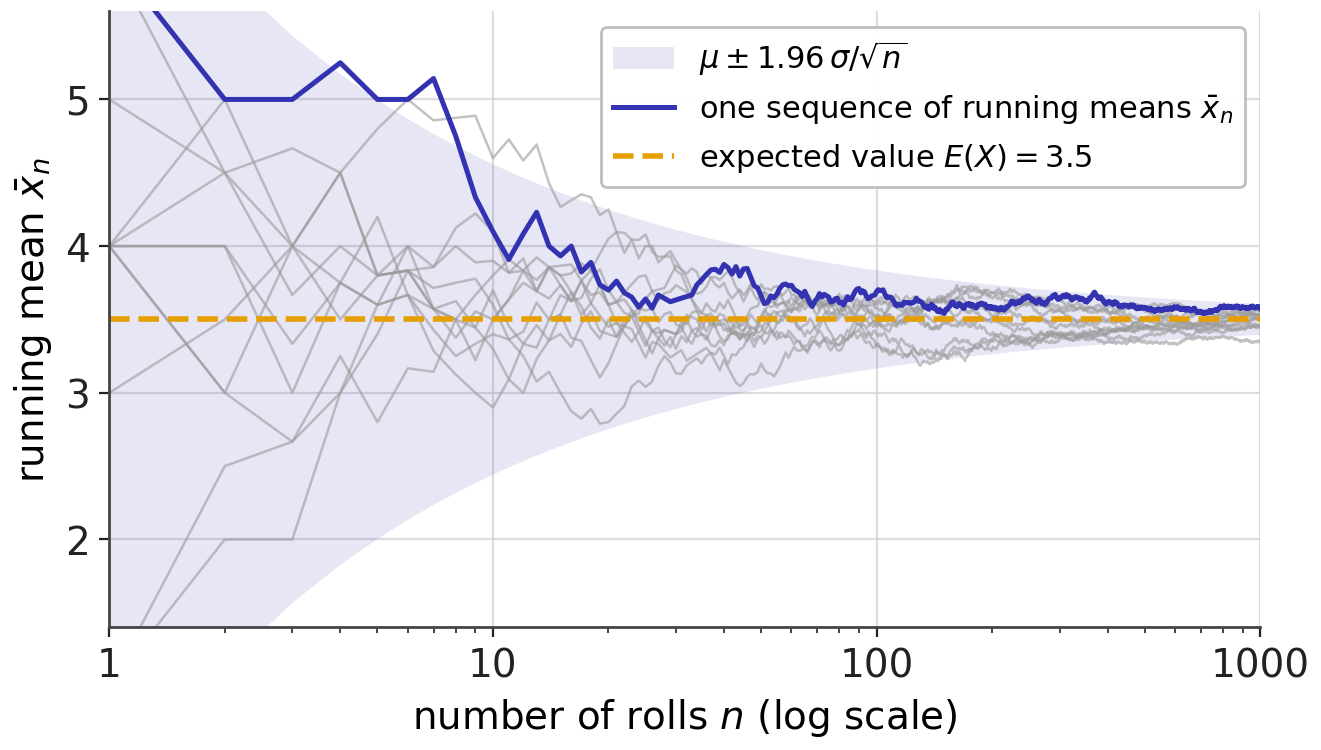
\includegraphics[width=\textwidth,height=0.62\textheight,keepaspectratio]{images/lln_running_mean.png}
    \end{column}
  \end{columns}
  \vspace{2pt}
  {\footnotesize Twelve sequences of die rolls (grey), one highlighted (blue).
  The funnel $\mu\pm1.96\,\sigma/\sqrt n$ narrows: $\pm1.06$ at $n=10$,
  $\pm0.33$ at $n=100$, $\pm0.11$ at $n=1000$.}
\end{frame}

\begin{frame}{The law of large numbers -- formal statement}
  \begin{block}{Weak law of large numbers}
    For i.i.d.\ $X_i$ with $E(X_i)=\mu$ and $\mathrm{Var}(X_i)=\sigma^2<\infty$:
    \[
      \lim_{n\to\infty}P\bigl(|\bar X_n-\mu|>c\bigr)=0
      \quad\text{for every } c>0,
      \qquad\text{i.e.}\quad \bar X_n\xrightarrow{\;P\;}\mu .
    \]
  \end{block}
  \inworten{Choose any tolerance $c$, however small: the probability that
  $\bar X_n$ misses $\mu$ by more than $c$ goes to zero.}\par
  {\small \textbf{Why?} Chebyshev's inequality:
  $P(|\bar X_n-\mu|>c)\le\mathrm{Var}(\bar X_n)/c^2=\sigma^2/(n\,c^2)\to0$.\par}
  \begin{exampleblock}{Special case: relative frequencies (Bernoulli)}
    $X_i=1$ if an event occurs (probability $p$), else $0$: then $\bar X_n$ is
    the event's \emph{relative frequency}, and $\bar X_n\xrightarrow{P}p$ --
    the basis of the \textbf{frequentist} view used throughout this part.
  \end{exampleblock}
  {\footnotesize LLN: $\bar X_n$ approaches $\mu$. \ CLT: how the remaining
  fluctuation around $\mu$ is distributed.}
\end{frame}

\end{document}
